\documentclass[10pt]{article}

\usepackage[margin=0.9in]{geometry}
\usepackage{amsmath,amssymb,mathtools,amsthm}
\usepackage{booktabs}
\usepackage{array}
\usepackage{enumitem}
\usepackage{graphicx}
\graphicspath{{../}}% figures/ lives one level up from papers/
\usepackage{float}
\usepackage[section]{placeins}
\usepackage{listings}
\usepackage{tabularx}
\usepackage{needspace}
\usepackage{microtype}
\usepackage[font=small,labelfont=bf,margin=0.5cm]{caption}
\usepackage{xcolor}
\usepackage{algorithm}
\usepackage{algpseudocode}
\usepackage{tikz}
\usetikzlibrary{arrows.meta,positioning,calc}
\usepackage[colorlinks=true,linkcolor=blue!50!black,citecolor=blue!50!black,urlcolor=blue!50!black]{hyperref}
\renewcommand{\topfraction}{0.85}\renewcommand{\bottomfraction}{0.7}
\renewcommand{\textfraction}{0.15}\renewcommand{\floatpagefraction}{0.75}
\setlength{\emergencystretch}{3em}

% -- one set of theorem environments, numbered within section --
\theoremstyle{plain}
\newtheorem{theorem}{Theorem}[section]
\newtheorem{lemma}[theorem]{Lemma}
\newtheorem{proposition}[theorem]{Proposition}
\newtheorem{corollary}[theorem]{Corollary}
\theoremstyle{definition}
\newtheorem{definition}[theorem]{Definition}
\newtheorem{example}[theorem]{Example}
\theoremstyle{remark}
\newtheorem{remark}[theorem]{Remark}

% -- macros --
\newcommand{\R}{\mathbb{R}}
\newcommand{\E}{\mathbb{E}}
\newcommand{\Prob}{\mathbb{P}}
\newcommand{\T}{^{\top}}
\newcommand{\opn}[1]{\lVert #1\rVert_2}
\newcommand{\fro}[1]{\lVert #1\rVert_F}
\newcommand{\norm}[1]{\lVert #1\rVert}
\newcommand{\obs}{\mathcal{O}}
\DeclareMathOperator{\tr}{tr}
\DeclareMathOperator{\rank}{rank}
\DeclareMathOperator{\range}{range}
\DeclareMathOperator*{\argmin}{arg\,min}
\DeclareMathOperator{\osc}{osc}
\newcommand{\softmax}{\operatorname{softmax}}
\newcommand{\dmodel}{d_{\mathrm{model}}}
\newcommand{\dhead}{d_{\mathrm{head}}}
\newcommand{\kbe}{k_{\mathrm{be}}}
\newcommand{\epsEY}{\varepsilon_{\mathrm{EY}}}
\newcommand{\mtx}[1]{\texttt{#1}}
\newcommand{\plain}{\noindent\emph{In plain words.}\ }
\newcommand{\means}{\noindent\textbf{What it means.}\ }
\newcommand{\rl}[1]{\textsf{#1}}% name of a rule fixed in advance (keeps rule names apart from symbols)

\lstset{basicstyle=\ttfamily\footnotesize,columns=fullflexible,keepspaces=true,
  breaklines=true,numbers=left,numberstyle=\tiny,frame=lines,showstringspaces=false,
  language=Python}

\title{Low-Rank Compression of LLM Weights and the KV Cache\\[4pt]
\large Theory of the SVD, ALS and Randomized SVD, and Experiments on GPT-2}
\author{Anikait Rao, Ayush Manocha, Sucheta Sarangi}
\date{November 25, 2026}

\begin{document}
\maketitle

\begin{abstract}
\noindent Most of the memory of a running large language model sits in its \emph{weight matrices} and in the \emph{key--value (KV) cache}, which stores information about every earlier token. We study one tool for shrinking both: \emph{low-rank factorization}. We first prove the theory: the singular value decomposition (SVD), alternating least squares (ALS) for matrices with missing entries, and the randomized SVD (RSVD). On GPT-2 small, the weights are \emph{not} close to low rank, and weight error is a misleading guide: plain factorization at 90\% of the parameters raises perplexity (lower is better) from $33.6$ to $1689$, while an activation-aware SVD gives $40.1$. The error on a layer's outputs is a better but imperfect guide: it ranks methods of one size well, but not across sizes. For the KV cache, one basis per layer shared by all heads halves the cache at $+4.0\%$ perplexity, for $6\times$ the attention arithmetic. A basis computed from the prompt, updated during generation, with the newest tokens kept exact, costs $+0.2\%$ while storing half as many numbers per token, also on fresh text and after a short prompt, and is as good as an offline basis calibrated on the same kind of text (one mild domain shift, GPT-2 only). Counting the per-prompt basis, its memory is $0.92$ of the full cache at 1024 tokens, and plain 8- or 4-bit quantization reaches the same quality at much lower memory (quantizing the low-rank codes with scales grouped over tokens adds no loss but does not beat plain 4-bit). On a small model with rotary positions (SmolLM2-135M) the same recipe costs $+4.6\%$; there an attention-weighted prompt basis does better than the update, and the two combined (chosen post hoc, confirmed on new windows) reach about $+1.0$ to $+1.2\%$; quantization is again the stronger use of memory there. This recipe was published shortly before, on larger models. Our contribution is analysis on GPT-2: the newest tokens must be kept exact because they are recent, not merely because they are new to the basis; buffer and update complement each other; new tokens fit the basis worse than the prompt, through out-of-sample error and drift of the text; the attention-sink key lies opposite the mean; and we measure how tight one-layer attention-output bounds are, while compressing all 12 layers costs $1.57$ times the sum of the single-layer excess losses.
\par\medskip\noindent\textbf{Keywords:} low-rank approximation, singular value decomposition, randomized SVD, alternating least squares, LLM compression, KV cache, GPT-2, perplexity.
\end{abstract}

\tableofcontents
\newpage

% =====================================================================
% ---- begin short/s01_intro ----
\section{Introduction}
\label{sec:intro}
% =====================================================================

\paragraph{The problem.}
Large language models (LLMs) are expensive to run. A model's \emph{parameters} (or \emph{weights}) are the numbers it learned during training. A model with 7 billion of them in a 16-bit (2-byte) format takes about $14$~GB, and generating each word requires reading all of them from memory, which caps the speed (Section~\ref{sec:cost}). The model also keeps a \emph{KV cache}, a store of information about every earlier token, which grows with the length of the text and the number of users and can exceed the weights in size (Section~\ref{sec:kvcache}). Smaller weights and caches mean cheaper, faster generation on smaller hardware.

\paragraph{The tool.}
Almost all of these bytes sit in large matrices (rectangular tables of numbers). A matrix $W$ with $m$ rows and $n$ columns can be replaced by the product $UV\T$ of two thin matrices, $U$ with $m$ rows and $V$ with $n$ rows, each with only $k$ columns. This is a \emph{rank-$k$ factorization}. It stores $k(m+n)$ numbers instead of $mn$, and multiplying a vector by it costs $k(m+n)$ multiply-adds instead of $mn$. Section~\ref{sec:theory} develops three algorithms for it, with proofs: the truncated \emph{singular value decomposition} (SVD), which gives the best possible rank-$k$ approximation; the \emph{randomized SVD} (RSVD), a fast approximation of it for large matrices whose entries are all known; and \emph{alternating least squares} (ALS), which fits only the known entries of a matrix with missing entries.

\paragraph{The question.}
Are the weights and the KV cache of a real language model close enough to low rank for factorization to save memory without damaging the model? And do the algorithms behave on them as the theory predicts? We answer both for GPT-2 small, a model with 124 million parameters \cite{radford2019}, on a laptop CPU.

\paragraph{Organization.}
Section~\ref{sec:llm} gives the background and our conventions, Section~\ref{sec:theory} the theory, and Section~\ref{sec:weights} the weight experiments. The KV cache follows: is it low rank, and can attention heads share a basis (Section~\ref{sec:kv}); a basis computed from the prompt (Section~\ref{sec:kvonline}); bounds on the error in the attention output (Section~\ref{sec:kvbound}); a basis updated during generation (Section~\ref{sec:kvupdate}). Section~\ref{sec:discussion} gives limitations and future work; the appendices hold proofs, extra results with the list of all test rules, reproduction instructions and a glossary. Terms are explained at first use; the glossary lists the specialised ones (Appendix~\ref{app:glossary}); \emph{In plain words} and \emph{What it means} paragraphs give the ideas without formulas. How tests were judged (rules fixed before the run, rule names such as \rl{R1}, \emph{post hoc}) is explained in Section~\ref{sec:measure}.

\paragraph{Main findings.}
\begin{itemize}[leftmargin=2em,itemsep=1pt]
\item \textbf{The theory holds on real matrices.} Every inequality we checked held on GPT-2's weights and caches. RSVD was up to $54\times$ faster than the exact SVD (up to $63\times$ in an idle-CPU rerun) with nearly optimal error, though its probabilistic error bounds were too loose to be informative.
\item \textbf{GPT-2's weights are not close to low rank.} Keeping 95\% of a matrix's ``energy'' needs about as much rank as it takes for the factorization to stop saving memory. ALS cannot predict pruned (deleted) weights.
\item \textbf{Weight error is a misleading guide; measure error on the inputs a layer actually sees.} Plain factorization breaks the model even at 90\% of its size (perplexity $33.6\to1689$); an activation-aware SVD gives $40.1$. Output error is a better guide but not a perfect one: it ranks the methods of one size almost perfectly, yet plain SVD at 90\% of the size has a \emph{smaller} output error than the activation-aware SVD at 50\% ($0.205$ vs.\ $0.260$) and a far worse perplexity ($1689$ vs.\ $214$).
\item \textbf{The KV cache is not low rank head by head} (a no-go by our rule), but \textbf{one basis per layer, shared by all 12 heads, halves the cache at $+4.0\%$ perplexity} ($+3.9\%$ on fresh text). The price is about $6\times$ more arithmetic in attention, which makes one decode step at 4k--64k cached tokens $1.3$--$1.5\times$ slower on our CPU ($1.2$--$1.35\times$ in an idle rerun).
\item \textbf{Headline: a basis computed from the prompt and updated during generation costs $+0.2\%$ while storing half as many numbers per token.} The recipe takes an exact SVD of the prompt, updates the basis by an incremental SVD every 32 tokens, keeps the newest tokens exact, and needs no calibration text; it is as good as an offline basis calibrated on the same kind of text, and much better than one calibrated on another kind (one mild change of domain; Section~\ref{sec:kvadditive}). The $+0.2\%$ holds on fresh text ($+0.21\%$) and after a 256-token prompt ($+0.20\%$). Half refers to the stored codes only: each prompt also needs its own basis, so counted in full (Proposition~\ref{prop:kvmem}) the cache takes $0.92$ of the full cache's memory at GPT-2's 1024 tokens and saves memory only beyond about 870 tokens (an offline basis needs no per-prompt storage: $0.52$ of the memory, at $+1.2\%$). Three further caveats:
\begin{enumerate}[leftmargin=2em,itemsep=0pt,label=(\roman*)]
\item it uses an exact SVD of the prompt; with RSVD it is $+0.3\%$;
\item it does not carry over to the small rotary-position model SmolLM2-135M, where it is $+4.6\%$ and an attention-weighted prompt basis does better ($+1.75\%$; combined with the update, a post hoc choice, $+0.98\%$, confirmed on 16 fresh windows: $+1.15\%$);
\item a larger exact buffer alone does about as well: 128 tokens give $+0.07\%$ on fresh text, at $0.97$ of the memory, statistically indistinguishable from the updated cache.
\end{enumerate}
\item \textbf{Simpler methods reach the same quality at much lower memory on GPT-2.} Quantizing the cache to 8 bits costs $+0.002\%$ at $0.56$ of the memory, and to 4 bits $+0.10\%$ at $0.32$, against $+0.20\%$ at $0.92$ for the updated low-rank cache; 8-bit is borderline better than the updated cache, and the other differences are within the variation between windows (Section~\ref{sec:kvchecks}). Low rank and 8-bit codes combine without loss ($+0.20\%$ at $0.71$) only with scales grouped over tokens; with one scale per token the update loses $+2.2\%$ (Section~\ref{sec:kvround3}). On SmolLM2, too, 4-bit ($+0.60\%$ at $0.30$) is ahead of the best low-rank cell.
\item \textbf{We prove bounds} from the cache error to the attention output. The variance form is a median $2.6\times$ the actual error on real attention ($2.4\times$ when the smaller of the two forms is taken for each term) and orders our 10 test settings like the actual error does; the weaker bounds order them no better than a trivial residual proxy. The bounds cover one layer; compressing all 12 layers costs $1.57$ times the sum of the single-layer excess losses (Section~\ref{sec:kvadditive}).
\end{itemize}

\paragraph{What is known and what is new.}
We checked the literature after the experiments. Several of our designs had been reached earlier by others, and we say so wherever they appear. The activation-aware SVD of the weights is known \cite{wang2025svdllm,yuan2023asvd}. The main KV-cache recipe (a basis computed from the prompt, shared by the heads of a layer, updated by an incremental SVD, with the newest tokens exact) is close to iS-KV \cite{iskv2026} and AttSVD \cite{attsvd2026}, found only afterwards; we call it \emph{independently reached, close to iS-KV and AttSVD}, not new. What we did not find elsewhere is analysis:
\begin{enumerate}[leftmargin=2em,itemsep=0pt]
\item a planned test that separates the exact recent buffer from the basis update, and controls showing that the buffer works because its tokens are recent;
\item a measurement of how much worse new tokens fit the basis than the prompt, split into out-of-sample error and drift of the text;
\item on GPT-2, weighting the prompt basis by attention does not help, and why; on a small rotary-position model it does;
\item the geometry of the ``attention sink'' key on GPT-2;
\item how tight attention-output bounds are on real attention, and why.
\end{enumerate}
Section~\ref{sec:novelty} gives each item in detail.

% =====================================================================

% ---- end short/s01_intro ----
% ---- begin short/s02_background ----
\section{Background: language models and the KV cache}
\label{sec:llm}
% =====================================================================

\subsection{What a language model computes}
\label{sec:transformer}

\paragraph{Next-token prediction.}
Text is cut into \emph{tokens}: words or pieces of words, such as ``compress'' + ``ion''. Given the tokens so far, $x_1,\dots,x_t$, the model outputs a probability for every possible next token $x_{t+1}$ in its vocabulary; the raw scores before they become probabilities are called \emph{logits}. To generate text, the model picks a likely token, appends it, and repeats.

\paragraph{The transformer.}
Modern LLMs are \emph{transformers} \cite{vaswani2017}. Each token is turned into a vector (a list) of $\dmodel$ numbers, $x\in\R^{\dmodel}$, that represents its meaning in context ($\dmodel=768$ for GPT-2 small). This vector passes through $L$ blocks of the same design, called \emph{layers} ($L=12$), each with two parts.
\begin{enumerate}[leftmargin=2em,itemsep=1pt]
\item \textbf{Self-attention} lets each token gather information from earlier tokens. Three learned $\dmodel\times\dmodel$ weight matrices turn the token's vector into a \emph{query} $q=xW_Q$ (what the token is looking for), a \emph{key} $k=xW_K$ (what it offers) and a \emph{value} $v=xW_V$ (the information it passes on). With the keys $k_1,\dots,k_t$ and values $v_1,\dots,v_t$ of all tokens so far, the output is
\begin{equation}\label{eq:attn}
o=\sum_{i=1}^{t}a_i v_i,\qquad
a=\softmax(s),\quad s_i=\frac{q\cdot k_i}{\sqrt{\dhead}},\quad a_i=\frac{e^{s_i}}{\sum_je^{s_j}},
\end{equation}
which is then multiplied by an \emph{output matrix} $W_O$. In words: $q\cdot k_i$ \emph{scores} how well token $i$ matches the query, the \emph{softmax} turns the scores into positive \emph{attention weights} $a_i$ that sum to 1, and the output is the weighted average of the values. The vectors are split into $H$ pieces called \emph{heads}, each of size $\dhead=\dmodel/H$ ($H=12$, $\dhead=64$ for GPT-2 small); each head computes its own~\eqref{eq:attn}, so different heads can attend to different things.
\item \textbf{The feed-forward network (MLP)} transforms each token's vector on its own: $x\mapsto\phi(xW_1)W_2$, with a fixed nonlinear function $\phi$ applied to each entry (GPT-2 uses GELU, a smooth version of $\max(0,z)$) and weight matrices $W_1$, $W_2$ of sizes $\dmodel\times4\dmodel$ and $4\dmodel\times\dmodel$.
\end{enumerate}
In all model sections a token's vector is a \emph{row}, and a layer multiplies it from the right, $x\mapsto xW+b$, with a learned \emph{bias} vector $b$. (The theory in Section~\ref{sec:theory} uses column vectors; nothing depends on this choice.)

\paragraph{GPT-2's weight matrices.}
A layer of GPT-2 holds four large weight matrices, named as in the code:
\mtx{attn.c\_attn} ($768\times2304$) is $W_Q$, $W_K$, $W_V$ side by side;
\mtx{attn.c\_proj} ($768\times768$) is the output matrix $W_O$;
\mtx{mlp.c\_fc} ($768\times3072$) and \mtx{mlp.c\_proj} ($3072\times768$) are $W_1$ and $W_2$ of the MLP.
The $12\times4=48$ matrices hold $84.9$ of GPT-2's $124.4$ million parameters ($68\%$); most of the rest is the \emph{embedding}, which turns each of the $50{,}257$ vocabulary tokens into a vector.

\paragraph{Positions.}
Attention by itself does not know the order of the tokens. GPT-2 adds a learned \emph{position vector} to each token's vector at the input, so its keys are plain products $xW_K$. Many newer models instead rotate each query and key by an angle that depends on the token's position (\emph{rotary position encoding}, RoPE \cite{su2024rope}), so their cached keys change with position; we return to this in Section~\ref{sec:discussion}.

\subsection{Why running a language model is expensive}
\label{sec:cost}

Running a trained model to answer requests is called \emph{inference}. In its first phase, \emph{prefill}, the model reads the whole prompt at once; this is limited by how fast the chip does arithmetic. In the second, \emph{decode}, it produces the answer one token at a time, running the whole network on a single vector per step. Decode is the slow phase. Each weight is read from memory once (2 bytes) and used for about 2 operations (one multiply, one add), so about 1 operation per byte read. A typical data-center GPU (graphics processing unit, the chip LLMs normally run on), the NVIDIA A100, can do about $3\times10^{14}$ such operations per second, but its memory delivers only about $2\times10^{12}$ bytes per second, its \emph{memory bandwidth} \cite{nvidia2020}. The arithmetic units therefore mostly wait for data: decode is \emph{memory-bound} \cite{pope2023}, with the speed limit
\begin{equation}\label{eq:speed}
\text{time per token}\;\gtrsim\;\frac{\text{bytes read per token}}{\text{memory bandwidth}}.
\end{equation}
For a 7-billion-parameter model in 16-bit numbers, $1.4\times10^{10}\,\text{B}/(2\times10^{12}\,\text{B/s})=7$~ms, i.e.\ at most about $140$ tokens per second. \emph{Fewer bytes per token means faster generation}, and fewer bytes in total means fewer GPUs.

\subsection{The KV cache}
\label{sec:kvcache}

In~\eqref{eq:attn}, generating token $t+1$ needs the keys and values of all earlier tokens. They do not change as generation continues, so the model stores them once per layer and reuses them. This store is the \emph{KV cache} (key--value cache) \cite{pope2023}; Figure~\ref{fig:decode} shows one decode step. It saves recomputation, but grows by one key and one value per layer and head with every token.

\begin{figure}[!tb]
\centering
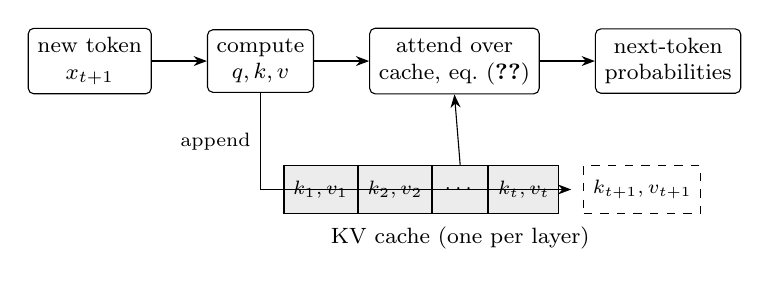
\begin{tikzpicture}[
  box/.style={draw, rounded corners=2pt, minimum height=7mm, align=center, font=\footnotesize},
  cache/.style={draw, fill=gray!15, minimum height=6mm, minimum width=7mm, font=\scriptsize},
  >=Stealth]
\node[box] (tok) {new token\\ $x_{t+1}$};
\node[box, right=7mm of tok] (proj) {compute\\ $q,k,v$};
\node[box, right=7mm of proj] (att) {attend over\\ cache, eq.~\eqref{eq:attn}};
\node[box, right=7mm of att] (out) {next-token\\ probabilities};
\draw[->] (tok) -- (proj);
\draw[->] (proj) -- (att);
\draw[->] (att) -- (out);
\node[cache, below=9mm of att, xshift=-17mm] (c1) {$k_1,v_1$};
\node[cache, right=0mm of c1] (c2) {$k_2,v_2$};
\node[cache, right=0mm of c2] (c3) {$\cdots$};
\node[cache, right=0mm of c3] (c4) {$k_t,v_t$};
\node[cache, right=3mm of c4, fill=white, dashed] (c5) {$k_{t+1},v_{t+1}$};
\draw[->] (c3.north) -- (att.south);
\draw[->] (proj.south) |- ($(c5.west)+(-1.5mm,0)$) node[pos=0.25, left, font=\scriptsize] {append};
\node[font=\footnotesize, below=0.5mm of c3] {KV cache (one per layer)};
\end{tikzpicture}
\caption{One decode step. The new token's query is compared with the keys of all earlier tokens, which are read from the cache, and the new token's own key and value are appended to the cache for later steps.}
\label{fig:decode}
\end{figure}

\begin{proposition}[KV-cache size]\label{prop:kvsize}
With $L$ layers, $H_{kv}$ key--value heads of dimension $\dhead$, $b$ bytes per number, and $N_{\mathrm{seq}}$ sequences of $T$ tokens,
\[
\text{KV bytes}=2\cdot L\cdot H_{kv}\cdot\dhead\cdot b\cdot T\cdot N_{\mathrm{seq}} .
\]
\end{proposition}
\begin{proof}
Per token and layer, the cache holds a key and a value of $H_{kv}\dhead$ numbers each; multiply by $b$, $L$, $T$ and $N_{\mathrm{seq}}$.
\end{proof}

The cache grows in proportion to the \emph{context length} $T$ (the number of tokens the model keeps track of) and the \emph{batch size} $N_{\mathrm{seq}}$ (the number of sequences or users served at once; the letter $B$ is kept for the block size of Section~\ref{sec:kvupdate}). With 2 bytes per number, GPT-2 small ($L=H_{kv}=12$, $\dhead=64$) needs 36~KiB per token, or 144~MiB for one sequence of $T=4096$ tokens; Llama-2-7B \cite{touvron2023} ($L=H_{kv}=32$, $\dhead=128$) needs 512~KiB per token and 2~GiB; Llama-2-70B ($L=80$, $\dhead=128$) shares each key--value head among several query heads (grouped-query attention, Section~\ref{sec:families}), so $H_{kv}=8$ and it needs 320~KiB per token and 1.25~GiB (KiB, MiB, GiB are $2^{10}$, $2^{20}$, $2^{30}$ bytes). Serving Llama-2-7B to $N_{\mathrm{seq}}=16$ users with $4096$-token contexts thus needs $14$~GB of weights but $16\times2=32$~GiB of cache. The cache, not the weights, then decides how many users fit on a GPU \cite{kwon2023vllm}, and since each sequence reads its own cache at every decode step, for large batches and long contexts it also dominates the memory traffic in~\eqref{eq:speed} \cite{pope2023}.

\subsection{How models and caches are compressed}
\label{sec:families}

Every compression method reduces the bytes stored and read while changing the model's outputs as little as possible; savings of different methods multiply when they are combined.

\paragraph{Weights.}
\emph{Quantization} stores each weight with fewer bits, for example 4 instead of 16 (rounding it to one of $2^4$ levels, about $4\times$ smaller). Methods such as GPTQ \cite{frantar2023gptq} and AWQ \cite{lin2024awq} use \emph{calibration data}, a small sample of real text run through the model to see which weights matter most. \emph{Pruning} sets many weights to zero, for example the smallest ones (\emph{magnitude pruning}) \cite{han2016}; the surviving entries form a matrix with ``missing'' entries. \emph{Low-rank factorization}, our subject, replaces $W$ by $UV\T$; variants for LLMs weight the error by the typical inputs (\emph{activations}) a layer receives \cite{hsu2022,wang2025svdllm,yuan2023asvd}.

\paragraph{The KV cache.}
Each family shrinks one factor of Proposition~\ref{prop:kvsize}.
\emph{Fewer heads ($H_{kv}$):} in multi-query and grouped-query attention (MQA, GQA) \cite{shazeer2019,ainslie2023} several query heads share one key--value head, and DeepSeek-V2 caches one small compressed vector per token, from which keys and values are recomputed (multi-head latent attention, MLA) \cite{deepseek2024}; these must be built in during training.
\emph{Fewer bits ($b$):} KIVI quantizes the cache to 2 bits per number \cite{liu2024kivi}.
\emph{Fewer tokens ($T$):} H2O \cite{zhang2023h2o} keeps only the most-attended and the most recent tokens and \emph{evicts} (deletes) the rest.
\emph{Smaller vectors ($\dhead$), the family we study:} the keys of one head form a matrix with one row of $\dhead$ numbers per token; if the rows lie close to a subspace of dimension $r\ll\dhead$, the cache can store $r$ numbers per token instead of $\dhead$ (Loki \cite{singhania2024loki}, Palu \cite{palu2025}; Section~\ref{sec:relwork}).
Key errors enter through the exponent of the softmax in~\eqref{eq:attn} and can change the attention weights by large factors, while value errors enter the output linearly; so methods, ours included, treat keys and values differently.

\paragraph{The memory of a low-rank cache.}
A low-rank cache stores, for each token, a short \emph{code} (its coordinates in a basis) instead of the full key and value. The basis must be stored too. A basis computed once from calibration text and shared by all sequences (an \emph{offline} basis) is a fixed part of the model; a basis computed from each prompt (an \emph{online} basis, Sections~\ref{sec:kvonline}--\ref{sec:kvupdate}) is stored once per sequence. The next proposition counts both.

\begin{proposition}[Memory of a factored cache]\label{prop:kvmem}
Take one layer and one sequence of $T$ tokens, with keys and values of $d=H\dhead$ numbers each. Suppose the keys are stored as codes of $R_K$ numbers and the values as codes of $R_V$ numbers ($R=d$ for a kind that is not compressed), $n_{\mathrm{ex}}$ tokens are stored exactly, and the sequence also stores $M$ numbers of side information. Assume $n_{\mathrm{ex}}\le T$ and $R_K+R_V<2d$. Then the memory of the factored cache relative to the full cache is
\[
\rho(T)=\rho_0+\frac{M+n_{\mathrm{ex}}\,(2d-R_K-R_V)}{2dT},\qquad \rho_0=\frac{R_K+R_V}{2d},
\]
and the factored cache is smaller than the full one if and only if $T>T^\ast=\dfrac{M+n_{\mathrm{ex}}(2d-R_K-R_V)}{2d-R_K-R_V}$. For a per-sequence basis, $M=\sum_{\kappa}(dR_\kappa+d+R_\kappa)+n_G$, where the sum runs over the \emph{compressed} kinds $\kappa\in\{K,V\}$ only: the basis vectors, the mean, and the singular values that the basis update of Section~\ref{sec:kvupdate} needs. $n_G=H\dhead^2$ counts the block-diagonal key weight $G_K^{1/2}$ of Section~\ref{sec:recipe} if the keys are compressed and $G_K$ is computed from the prompt; otherwise $n_G=0$. For an offline basis, $M=0$ per sequence.
\end{proposition}
\begin{proof}
The full cache stores $2dT$ numbers. The factored cache stores $(T-n_{\mathrm{ex}})(R_K+R_V)$ code numbers, $2dn_{\mathrm{ex}}$ exact numbers and $M$ side numbers, which is $T(R_K+R_V)+n_{\mathrm{ex}}(2d-R_K-R_V)+M$. Divide by $2dT$. The condition $\rho(T)<1$ rearranges to $T(2d-R_K-R_V)>M+n_{\mathrm{ex}}(2d-R_K-R_V)$.
\end{proof}

\plain The codes give the long-run saving $\rho_0$; the basis is a fixed cost per sequence, which pays off only for long texts. For GPT-2 ($d=768$, $H=12$, $\dhead=64$) at half the codes (keys $R_K=256$, values $R_V=512$) with a per-prompt basis and query weight, $M=641{,}280$ numbers per layer, more than the codes of 800 tokens. With the first token exact, $\rho=0.908$ at $T=1024$, $0.704$ at $2048$ and $0.551$ at $8192$; it reaches $0.5$ only as $T\to\infty$, and the cache saves memory only beyond $T^\ast=836$ tokens. With the 32-token buffer of Section~\ref{sec:kvupdate} it is $0.924$ at 1024 tokens ($T^\ast=868$). Variants at 1024 tokens: a shared key weight gives $0.877$ (no buffer), a third of the codes (keys $128$, values $384$) $0.617$, keys alone at $R_K=256$ $0.824$, and folding $G_K^{1/2}$ into $U_K$ $1.002$ (no help). An offline basis costs nothing per sequence: $0.500$ ($0.516$ with the buffer), plus a one-time $7.7$ million numbers for all 12 layers (without the value weight $G_V^{\pm1/2}$; with full encode and decode matrices for both kinds about $14.2$ million, small next to the model's 124 million parameters). The numbers come from \texttt{experiments/kv\_memory.py}.\footnote{Counting conventions: $n_G$ counts all entries of the symmetric $64\times64$ blocks (only the independent ones, $H\dhead(\dhead+1)/2=24{,}960$, would give $0.893$ instead of $0.908$); only one of $G_K^{1/2}$, $G_K^{-1/2}$ is counted (both: $0.939$); the static and online bases do not need the singular values, which changes $\rho$ by $0.0005$. Our code stores $G^{\pm1/2}$ as dense $768\times768$ matrices for convenience; the counts use the block-diagonal entries a real cache needs.} The break-even length grows with the width of the cache, so ``the basis is too large'' is partly an artefact of GPT-2's 1024 tokens. From the same formula (computed, not measured; \texttt{experiments/rerun\_2026-11-22/memory\_other\_models.py}): for SmolLM2-135M ($d=192$ over 3 key--value heads, keys 64 and values 128, with the 32-token buffer) $M=49{,}728$ numbers per layer, $\rho=0.548$ at 3072 tokens and $T^\ast=292$; for an 8B-sized model with 8 key--value heads of size 128 and half the numbers per token, $T^\ast\approx1190$ tokens and $\rho=0.645$, $0.573$ and $0.518$ at 4096, 8192 and 32{,}768 tokens. The tables of Sections~\ref{sec:kvonline}--\ref{sec:kvupdate} give this memory next to the share of codes kept.

\subsection{How we measure quality, and other conventions}
\label{sec:measure}

\paragraph{Perplexity.}
The standard quality measure is \emph{perplexity} on text the model has not seen: the exponential of the average negative log-probability that the model assigns to each true next token. Roughly, it is the number of tokens the model is ``choosing between'' at each step, so \emph{lower is better}. A model that always gave the true token probability $1/34$ would have perplexity 34. Uncompressed GPT-2 scores $33.64$ on our test text. A change of $+5\%$ is small but noticeable; a perplexity in the hundreds or thousands means the model is broken. The average negative log-probability itself is the \emph{loss}, measured in \emph{nats} (units of the natural logarithm); an excess loss of $x$ nats per token is a perplexity ratio of $e^x$, so $+0.01$ nats per token is about $+1\%$ perplexity.

\paragraph{Data.}
We use WikiText-2 \cite{merity2017}, a standard collection of Wikipedia articles. Perplexity is measured on \emph{windows} of $1024$ tokens (GPT-2's maximum context) from its test part: the first 8 windows ($8192$ tokens) unless stated otherwise, and windows 8--15 for confirmation runs on fresh text. Sections~\ref{sec:kvonline}--\ref{sec:kvupdate} use windows 0--15 (some follow-ups only 0--7) and fresh windows 16--31 for confirmation. \emph{Calibration} statistics (averages over real inputs, used to tune a method) come from 16 random windows of the training part ($16{,}384$ tokens), so they never overlap the test text.

\paragraph{Computing.}
All runs use one laptop CPU (no GPU). Factorizations are computed in \emph{float64} (64-bit floating-point numbers, about 16 correct digits) and the model runs in \emph{float32} (32-bit, about 7 digits). Timings are medians of repeated runs; they vary between sessions on the same machine by up to $1.7\times$, so only ratios (``$1.3\times$ slower'') should be compared.

\paragraph{Statistics.}
We often report a \emph{median} (the middle value) over many cases, with a \emph{5--95\% range} (all but the lowest and highest 5\% of the cases). A \emph{Spearman rank correlation} compares two orderings: it is $1$ if sorting runs by one quantity sorts them exactly by the other, $0$ if the orderings are unrelated. The follow-up experiments (mostly in Section~\ref{sec:kvupdate}) also give \emph{paired bootstrap 95\% confidence intervals} (CI) for the ratio of two perplexities: the test windows are resampled with replacement 10{,}000 times, the ratio is recomputed each time, and the middle 95\% of the results is the interval. If it excludes 1, the difference is larger than the variation between windows. With only 16 windows such percentile intervals tend to be slightly too narrow, so intervals that only just exclude 1 (such as $0.99993$, $0.99998$ or $1.00007$ below) are borderline. Their half-widths range from about $0.04\%$ to $1\%$, typically $0.1$--$0.5\%$, so differences of a few tenths of a percent between methods are often not resolved, and the many comparisons are not corrected for multiple testing. We add how many windows each method won and an exact two-sided \emph{sign test} ($p$: the probability, if both methods were equal, of a split of wins at least this uneven in either direction).

\paragraph{Rules fixed in advance.}
For most experiments we wrote down, \emph{before} running them, what result would count as a success. These \emph{rules fixed in advance} protect against choosing the success criterion after seeing the numbers. Each rule is reported as PASS or FAIL as written, even when it fails narrowly. (For the early rules of Section~\ref{sec:kv} we could not confirm from the files that they were written before the run; all later rules are in the docstrings of the scripts.) Rules carry short names in sans-serif type, such as \rl{R1} or \rl{F2}. The follow-up experiments are numbered C1--C23 after their result files (for example \texttt{c15\_summary.json} for C15): C1--C13 add checks to Sections~\ref{sec:blockscheme}--\ref{sec:kvchecks}, C14--C18 form Section~\ref{sec:kvround3} and C19--C23 Section~\ref{sec:kvadditive}. Where a rule name would clash with an earlier one, it is prefixed with its experiment, as in \rl{C15-R1}. Tables~\ref{tab:rules} and~\ref{tab:rules2} in Appendix~\ref{app:extra} state every rule with its verdict, so the experiment sections give only the question, the verdict and the key numbers. Comparisons made only after seeing the results are marked \emph{post hoc} (``after the fact''); the most important of them were later repeated as planned tests or on fresh text.

% =====================================================================

% ---- end short/s02_background ----
% ---- begin short/s03_theory ----
\section{Low-rank approximation: theory}
\label{sec:theory}
% =====================================================================

This section states the three algorithms used in the rest of the report: the truncated SVD, alternating least squares (ALS) and the randomized SVD (RSVD). Each result comes with an explanation in plain words. The proofs and worked examples are in Appendix~\ref{app:proofs}; standard results whose proofs we omit are cited.

A matrix $A$ with $m$ rows and $n$ columns could record how $m$ users rate $n$ films, with $a_{ij}$ the rating of user $i$ for film $j$. A standard model explains each entry by a small number $k$ of hidden features: $a_{ij}\approx u_i\T v_j$, where $u_i$ and $v_j$ are lists of $k$ numbers and $u_i\T v_j=\sum_lu_{il}v_{jl}$ is their dot product. Stacking the $u_i$ as the rows of $U\in\R^{m\times k}$ and the $v_j$ as the rows of $V\in\R^{n\times k}$ gives $A\approx UV\T$, a \emph{matrix factorization} \cite{funk2006,paterek2007}. Two problems arise:
\begin{enumerate}[label=(P\arabic*),leftmargin=2.5em,itemsep=0pt]
\item \textbf{Every entry known, but the matrix is large.} The truncated SVD gives the best rank-$k$ approximation, but it costs on the order of $mn\min(m,n)$ operations \cite{golubvanloan2013}. RSVD \cite{halko2011} gets close to it much faster. For GPT-2, $A$ is a weight matrix or a matrix of cached keys or values.
\item \textbf{Only some entries known.} The SVD is not defined; ALS \cite{zhou2008,hu2008} fits only the known entries. For GPT-2, $A$ is a weight matrix after pruning.
\end{enumerate}

\subsection{Notation}
\label{sec:notation}
\begin{itemize}[leftmargin=2em,itemsep=0pt]
\item Vectors are columns here. $A\T$ is the \emph{transpose} (rows and columns swapped) and $I_k$ the $k\times k$ identity. Vectors are \emph{orthonormal} if each has length 1 and every two are perpendicular (dot product 0); a matrix $Q$ with orthonormal columns satisfies $Q\T Q=I$.
\item $\norm x=(\sum_ix_i^2)^{1/2}$ is the length of a vector. The \emph{spectral norm} $\opn A=\max_{\norm x=1}\norm{Ax}$ is the most $A$ can stretch a vector of length 1; the \emph{Frobenius norm} $\fro A=(\sum_{ij}a_{ij}^2)^{1/2}$ is the length of $A$ treated as one long list of numbers. $\fro{A-B}/\fro A$ is the \emph{relative error} of an approximation $B$. The \emph{trace} $\tr M$ is the sum of the diagonal entries; $\fro A^2=\tr(A\T A)$.
\item The \emph{rank} of $A$ is the number of independent directions in it, equivalently the smallest $k$ for which $A=UV\T$ with $k$ columns. $\sigma_1\ge\dots\ge\sigma_r>0$ are its nonzero singular values (Theorem~\ref{thm:svd}), $r=\rank A$, and $\sigma_j(B)$ are those of another matrix $B$.
\item A symmetric $M$ is \emph{positive semidefinite} ($M\succeq0$) if $x\T Mx\ge0$ for all $x$, and \emph{positive definite} ($M\succ0$, which makes it invertible) if $x\T Mx>0$ for all $x\ne0$; $M\succeq N$ means $M-N\succeq0$.
\item $\obs$ is the set of positions $(i,j)$ of the known (\emph{observed}) entries; $\obs_i$ lists the known columns of row $i$, and $\obs^j$ the known rows of column $j$.
\item A \emph{subspace} is a flat set of vectors through the origin (a line, a plane, \dots); $\range(A)$ is the subspace of all vectors $Ax$. \emph{Projecting} onto a subspace replaces a vector by its closest point in it.
\item $B^\dagger$ is the \emph{pseudoinverse}, the closest thing to an inverse for a non-square matrix: if $B\in\R^{k\times\ell}$ has $k$ independent rows, $B^\dagger=B\T(BB\T)^{-1}$ and $BB^\dagger=I_k$.
\item ``$O(mn\ell)$ operations'' means at most a constant times $mn\ell$ arithmetic operations. $\E$ is the expectation (average) and $\Prob$ a probability. In later sections $V$ also denotes the matrix of cached \emph{values}; the context makes the meaning clear.
\end{itemize}

\subsection{The singular value decomposition and its optimality}
\label{sec:svd}

\plain Every matrix can be taken apart into a sum of simple layers $\sigma_iu_iv_i\T$. Each layer has an input direction $v_i$, an output direction $u_i$ and a strength $\sigma_i$, the \emph{singular value}. The directions within each family are perpendicular, and the layers are sorted from strongest to weakest.

\begin{theorem}[Thin SVD \cite{golubvanloan2013}]\label{thm:svd}
Every $A\in\R^{m\times n}$ of rank $r$ can be written $A=U\Sigma V\T=\sum_{i=1}^r\sigma_i u_iv_i\T$, where $U=[u_1,\dots,u_r]\in\R^{m\times r}$ and $V=[v_1,\dots,v_r]\in\R^{n\times r}$ have orthonormal columns and $\Sigma=\operatorname{diag}(\sigma_1,\dots,\sigma_r)$ with $\sigma_1\ge\dots\ge\sigma_r>0$.
\end{theorem}

The $u_i$ are the \emph{left} and the $v_i$ the \emph{right singular vectors}. They are also eigenvectors: $A\T Av_i=\sigma_i^2v_i$ (an \emph{eigenvector} of a square matrix $M$ is a vector that $M$ only stretches, $Mv=\lambda v$, and $\lambda$ is its \emph{eigenvalue}).

\begin{lemma}[Norms in terms of singular values]\label{lem:norms}
$\opn{A}=\sigma_1$ and $\fro{A}^2=\sum_{i=1}^r\sigma_i^2$. More generally, $\norm{Ax}^2=\sum_i\sigma_i^2(v_i\T x)^2$ for every $x$.
\end{lemma}

So $\sigma_1$ is the most the matrix can stretch a vector, and $\sum_i\sigma_i^2$ is its total \emph{energy} $\fro A^2$. For $k<r$ the \emph{truncated SVD} keeps only the $k$ strongest layers, $A_k=\sum_{i=1}^k\sigma_iu_iv_i\T$. By Lemma~\ref{lem:norms} applied to the discarded part, its error is set by the discarded singular values (the \emph{tail}):
\begin{equation}\label{eq:tail}
\opn{A-A_k}=\sigma_{k+1},\qquad \fro{A-A_k}^2=\sum_{i>k}\sigma_i^2 .
\end{equation}

\begin{example}[A $2\times2$ SVD by hand]\label{ex:svd}
Let $A=\begin{psmallmatrix}3&0\\4&5\end{psmallmatrix}$. Then $A\T A=\begin{psmallmatrix}25&20\\20&25\end{psmallmatrix}$ has eigenvalues $45$ and $5$ with unit eigenvectors $v_1=\tfrac1{\sqrt2}(1,1)\T$, $v_2=\tfrac1{\sqrt2}(1,-1)\T$. Hence $\sigma_1=\sqrt{45}\approx6.708$, $\sigma_2=\sqrt5\approx2.236$, $u_1=Av_1/\sigma_1=\tfrac1{\sqrt{10}}(1,3)\T$ and $u_2=Av_2/\sigma_2=\tfrac1{\sqrt{10}}(3,-1)\T$. Check: $u_1\T u_2=0$ and $\fro A^2=9+16+25=50=45+5$. The best rank-one approximation is $A_1=\sigma_1u_1v_1\T=\tfrac32\begin{psmallmatrix}1&1\\3&3\end{psmallmatrix}$, and $\opn{A-A_1}=\sqrt5=\sigma_2$, as~\eqref{eq:tail} says.
\end{example}

\begin{theorem}[Eckart--Young--Mirsky \cite{eckartyoung1936,mirsky1960}]\label{thm:ey}
Let $B\in\R^{m\times n}$ have $\rank B\le k<r$. Then
\[
\opn{A-B}\ge\sigma_{k+1}=\opn{A-A_k},\qquad
\fro{A-B}^2\ge\sum_{i>k}\sigma_i^2=\fro{A-A_k}^2 .
\]
\end{theorem}

\plain Keeping the $k$ strongest SVD layers is the best any rank-$k$ approximation can do, in either norm, and the smallest possible error is set by the discarded singular values alone. This makes the truncated SVD the yardstick for every other method in this report.

\begin{lemma}[Projection is the best approximation within a subspace; cf.\ \cite{halko2011}]\label{lem:proj}
Let $Q\in\R^{m\times\ell}$ have orthonormal columns and $P=QQ\T$. Then for every $C\in\R^{\ell\times n}$,
$\opn{A-PA}\le\opn{A-QC}$ and $\fro{A-PA}\le\fro{A-QC}$.
\end{lemma}

\plain Within the span of $Q$, the best approximation drops a perpendicular onto that subspace; $P=QQ\T$, the \emph{orthogonal projector}, does this. So once RSVD has found a good subspace, projecting onto it is the best use of it.

\subsection{The factorization problem}
\label{sec:mf}

\begin{definition}[Regularized low-rank factorization]\label{def:mf}
Given the known entries $\{a_{ij}\}_{(i,j)\in\obs}$, a rank $k$ and a number $\lambda\ge0$, find $U\in\R^{m\times k}$ (rows $u_i\T$) and $V\in\R^{n\times k}$ (rows $v_j\T$) that minimize
\begin{equation}\label{eq:J}
J(U,V)=\sum_{(i,j)\in\obs}\bigl(a_{ij}-u_i\T v_j\bigr)^2+\lambda\bigl(\fro{U}^2+\fro{V}^2\bigr).
\end{equation}
\end{definition}

\plain The first sum adds up the squared gap between the true value $a_{ij}$ and the prediction $u_i\T v_j$, over the known entries only. The second term, the \emph{regularization}, is a penalty that grows with the size of the factors. It prevents \emph{overfitting}: using huge numbers to fit the known entries so closely that predictions for all other entries get worse. The constant $\lambda$ sets the strength of the penalty; $\lambda=0$ means none.

\begin{proposition}[Every entry known: the SVD gives a best factorization]\label{prop:fullobs}
If $\obs$ contains every position and $\lambda=0$, then $\min_{U,V}\fro{A-UV\T}^2=\sum_{i>k}\sigma_i^2$, attained at $U=U_k\Sigma_k^{1/2}$, $V=V_k\Sigma_k^{1/2}$ (the first $k$ columns of the SVD factors).
\end{proposition}

\plain Splitting each singular value evenly between the two factors (the square roots $\Sigma_k^{1/2}$) gives \emph{balanced} factors of similar size. Our code stores the factors this way.

\begin{proposition}[Factorizations are not unique]\label{prop:nonuniq}
For every orthogonal $R\in\R^{k\times k}$ ($R\T R=I$), $J(UR,VR)=J(U,V)$. For every invertible $R$, $(UR)(VR^{-\top})\T=UV\T$.
\end{proposition}

\plain Only the product $UV\T$ and the subspaces spanned by the columns are determined, not the individual columns. For the KV cache this means that only the \emph{subspace} a basis spans matters.

\begin{proposition}[Energy identity: small error $=$ large captured energy]\label{prop:energy}
Let $Q\in\R^{m\times k}$ have orthonormal columns. Then
\[
\fro{A-QQ\T A}^2=\fro{A}^2-\fro{Q\T A}^2 .
\]
Hence minimizing the error over $Q$ is the same as maximizing $\fro{Q\T A}^2$, and the best value is $\max_Q\fro{Q\T A}^2=\sum_{i\le k}\sigma_i^2$, attained at $Q=U_k$.
\end{proposition}

\plain The kept and the lost energy add up to the total, like the two legs of a right triangle and its hypotenuse. So making the error small is the same as keeping as much energy as possible. The fraction of energy kept, $\sum_{i\le k}\sigma_i^2/\fro A^2$, gives a simple way to choose $k$. We call $k_{0.95}$ the smallest $k$ that keeps 95\% of the energy; its relative error is at most $\sqrt{1-0.95}=0.224$.

\begin{proposition}[The penalty is a prior belief]\label{prop:map}
Suppose each known entry is $a_{ij}=u_i\T v_j+\eta_{ij}$ with independent bell-curve (Gaussian) noise $\eta_{ij}$ of spread $\sigma$, and that, before seeing data, the factor rows are believed to be independent Gaussians of spread $\tau$. Then the most probable factors given the data (the \emph{maximum a posteriori} estimate) are exactly the minimizers of $J$, with $\lambda=\sigma^2/\tau^2$.
\end{proposition}

\plain The penalty encodes the belief that the factors are small; it is stronger for noisy data ($\sigma$ large) or factors expected to be small ($\tau$ small).

\subsection{Alternating least squares}
\label{sec:als}

\paragraph{The idea.}
Minimizing $J$ over $U$ and $V$ together is hard, because $J$ multiplies the unknowns ($u_i\T v_j$). But with $V$ fixed, $J$ is a quadratic in $U$ whose minimum has a formula, and the same holds with the roles swapped. ALS alternates between these two easy problems. For row $i$, let $W_i$ be the matrix whose rows are the $v_j\T$ with $j\in\obs_i$, and $a_i$ the vector of the known entries of that row. Then
\begin{equation}\label{eq:Jsplit}
J(U,V)=\sum_{i=1}^m\Bigl(\norm{a_i-W_iu_i}^2+\lambda\norm{u_i}^2\Bigr)+\lambda\fro{V}^2 .
\end{equation}
With $V$ fixed, this is a \emph{sum of $m$ independent problems}, one per row of $U$, each using only that row's known entries.

\begin{theorem}[Closed-form row update]\label{thm:row}
Let $\lambda>0$, $W\in\R^{d\times k}$, $a\in\R^d$, and $f(u)=\norm{a-Wu}^2+\lambda\norm u^2$. Set $M=W\T W+\lambda I_k$. Then
(a) $M\succeq\lambda I_k\succ0$, and $f$ has the unique minimizer $u^\star=M^{-1}W\T a$;
(b) for all $u$, $f(u)-f(u^\star)=(u-u^\star)\T M(u-u^\star)\ge\lambda\norm{u-u^\star}^2$.
\end{theorem}

\plain Each row problem is a \emph{ridge regression}: a least-squares fit (choosing unknowns to minimize a sum of squared errors) plus the penalty $\lambda\norm u^2$. Part (a) gives the best row; it is unique when $\lambda>0$, even if the row has fewer than $k$ known entries. Part (b) says that any other $u$ is worse by at least $\lambda$ times its squared distance from the best one. By symmetry, the column update is $v_j^\star=(Z_j\T Z_j+\lambda I_k)^{-1}Z_j\T a^j$, where $Z_j$ has rows $u_i\T$ for $i\in\obs^j$ and $a^j$ holds the known entries of column $j$. Example~\ref{ex:k2} in Appendix~\ref{app:proofs} works one update by hand.

\begin{algorithm}[!tb]
\caption{Alternating least squares (ALS) for the objective~\eqref{eq:J}}\label{alg:als}
\begin{algorithmic}[1]
\Require known entries $\{a_{ij}\}_{(i,j)\in\obs}$, rank $k$, $\lambda>0$, tolerance $\delta>0$, starting $V_0\in\R^{n\times k}$
\State $t\gets0$
\Repeat
  \State $u_i\gets\bigl(W_i\T W_i+\lambda I_k\bigr)^{-1}W_i\T a_i$ for $i=1,\dots,m$ ($W_i$ from $V_t$) \Comment{$U$-step: $U_{t+1}=T(V_t)$}
  \State $v_j\gets\bigl(Z_j\T Z_j+\lambda I_k\bigr)^{-1}Z_j\T a^j$ for $j=1,\dots,n$ ($Z_j$ from $U_{t+1}$) \Comment{$V$-step: $V_{t+1}=S(U_{t+1})$}
  \State $t\gets t+1$
\Until{the decrease of $J(U_t,V_t)$ in the last sweep is below $\delta$ \textbf{or} $t$ reaches a maximum}
\State \Return $U_t,V_t$
\end{algorithmic}
\end{algorithm}

\paragraph{The algorithm.}
Algorithm~\ref{alg:als} alternates the two updates. One round of both is a \emph{sweep}; each update alone is a \emph{half-step}. A sweep costs $O(|\obs|k^2+(m+n)k^3)$ operations. All row problems are independent and can be solved in parallel, the main practical appeal of ALS \cite{zhou2008}. ALS needs a starting $V_0$. A random one is common; Remark~\ref{rem:hybrid} explains why a start from an SVD is better, and Example~\ref{ex:saddle} shows that $V_0=0$ must be avoided.

\paragraph{Convergence.}
Write $T(V)=\argmin_UJ(U,V)$ (``the best $U$ for this $V$'') and $S(U)=\argmin_VJ(U,V)$; by Theorem~\ref{thm:row} both are well defined when $\lambda>0$. ALS computes $U_{t+1}=T(V_t)$ and $V_{t+1}=S(U_{t+1})$. Let $c_0,c_1,c_2,\dots$ be the values of $J$ after every half-step: $c_{2t}=J(U_{t+1},V_t)$ and $c_{2t+1}=J(U_{t+1},V_{t+1})$. The results below do \emph{not} show that ALS finds the best possible factors.

\begin{theorem}[Monotone decrease]\label{thm:mono}
For $\lambda>0$, the sequence $(c_s)$ is non-increasing and bounded below by $0$, so it converges to a limit $J_\infty\ge0$.
\end{theorem}

\begin{corollary}[The stopping rule terminates]\label{cor:eps}
(a) For every $\varepsilon>0$ there is $N$ with $0\le c_s-J_\infty<\varepsilon$ for all $s\ge N$.
(b) For every $\delta>0$ there is $N$ with $c_s-c_{s+1}<\delta$ for all $s\ge N$, so the stopping rule of Algorithm~\ref{alg:als} is met after finitely many sweeps.
\end{corollary}

\plain Each half-step picks the best $U$ (or $V$) given the other, so $J$ never goes up; it cannot go below zero, so it levels off and the rule ``stop when $J$ improves by less than $\delta$'' always stops. There is no \emph{rate}: how many sweeps this takes is not known.

\begin{lemma}[Iterates are bounded]\label{lem:coer}
For $\lambda>0$, $J(U,V)\ge\lambda(\fro U^2+\fro V^2)$, so every iterate satisfies $\fro U^2+\fro V^2\le c_0/\lambda$, so the iterates have convergent subsequences (Bolzano--Weierstrass: any sequence in a bounded region has one).
\end{lemma}

\begin{lemma}[The updates are continuous]\label{lem:cont}
For $\lambda>0$, the maps $T$ and $S$ are continuous: a small change in $V$ causes only a small change in the best $U$, and vice versa.
\end{lemma}

\begin{theorem}[Every limit point of ALS is stationary]\label{thm:stat}
Let $\lambda>0$. Every limit point $(\bar U,\bar V)$ of the iterates $(U_{t+1},V_t)$ satisfies
$\bar U=T(\bar V)$, $\bar V=S(\bar U)$, $J(\bar U,\bar V)=J_\infty$ and $\nabla J(\bar U,\bar V)=0$.
\end{theorem}

\plain A \emph{limit point} is a point the iterates come back arbitrarily close to infinitely often. $\nabla J=0$ means that the slope (gradient) of $J$ is zero in every direction: the point is \emph{stationary}, so small changes cannot improve it. It may still be a \emph{saddle}, where $J$ goes down in some directions and up in others (next example). The argument is a case of \emph{block coordinate descent} \cite{grippo2000}.

\begin{example}[Stationary does not mean optimal]\label{ex:saddle}
Take one entry, $a_{11}=1$, $k=1$ and $0<\lambda<1$, so $J(u,v)=(1-uv)^2+\lambda(u^2+v^2)$. The point $(0,0)$ is stationary with $J=1$, but $J(t,t)=(1-t^2)^2+2\lambda t^2<1$ for small $t>0$, so it is a saddle. ALS started at $v_0=0$ gives $u_1=0$, then $v_1=0$, and stays there forever. \emph{Lesson:} never start ALS from all-zero factors.
\end{example}

\begin{remark}[What is known beyond this]\label{rem:alsknown}
Finding the true matrix needs extra assumptions. If the matrix is exactly low rank, its information is spread over many entries (\emph{incoherent}), and enough entries are observed at random, then alternating minimization started from an SVD converges to it \cite{jain2013,hardt2014}. Setting the unknown entries to zero and taking an SVD instead treats them as observed zeros, which biases the fit toward zero; $J$ sums only over the known entries and avoids this.
\end{remark}

\subsection{The randomized SVD}
\label{sec:rsvd}

\paragraph{The idea.}
For any vector $\omega$, $A\omega=\sum_i\sigma_i(v_i\T\omega)u_i$ is a combination of the left singular vectors. For a random $\omega$ the numbers $v_i\T\omega$ are all of similar size, so the \emph{large} $\sigma_i$ dominate: $A\omega$ points mostly along the strongest output directions. RSVD (Algorithm~\ref{alg:rsvd}) has two stages. \emph{Stage A} multiplies $A$ by $\ell=k+p$ random vectors and makes the results orthonormal (a \emph{QR factorization} returns orthonormal columns $Q$ with the same span). With high probability, $\range(Q)$ nearly contains the span of $u_1,\dots,u_k$ \cite{halko2011}. \emph{Stage B} squeezes $A$ into that subspace, $B=Q\T A$, which has only $\ell$ rows, and takes the exact SVD of this small matrix. The $p$ extra vectors (\emph{oversampling}) protect against unlucky random draws. The optional $q$ \emph{power iterations} multiply by $AA\T$ again, which strengthens the large directions relative to the small ones.

\begin{algorithm}[!tb]
\caption{Randomized SVD (Halko--Martinsson--Tropp \cite{halko2011})}\label{alg:rsvd}
\begin{algorithmic}[1]
\Require $A\in\R^{m\times n}$, target rank $k$, oversampling $p\ge0$, power iterations $q\ge0$; $\ell=k+p\le\min(m,n)$
\State Draw $\Omega\in\R^{n\times\ell}$ with independent standard Gaussian entries \Comment{Stage A: find a subspace}
\State $Y\gets(AA\T)^qA\,\Omega$ \Comment{$q=0$: $Y=A\Omega$}
\State $Q\gets$ orthonormal basis of $\range(Y)$ (thin QR of $Y$)
\State $B\gets Q\T A\in\R^{\ell\times n}$ \Comment{Stage B: exact SVD of the small matrix}
\State Compute the SVD $B=\tilde U\hat\Sigma\hat V\T$ and set $\hat U\gets Q\tilde U$
\State \Return the first $k$ singular triplets: $A\approx\hat U_k\hat\Sigma_k\hat V_k\T$
\end{algorithmic}
\end{algorithm}

\begin{lemma}[Stage B is exact]\label{lem:stageB}
If $Q$ has orthonormal columns and $B=Q\T A=\tilde U\hat\Sigma\hat V\T$, then $QQ\T A=(Q\tilde U)\hat\Sigma\hat V\T$ is an SVD of $QQ\T A$.
\end{lemma}

\begin{corollary}[Cost of cutting to rank $k$]\label{cor:trunc}
Let $\hat A_k$ be the output of Algorithm~\ref{alg:rsvd}. Then $\opn{A-\hat A_k}\le\opn{A-QQ\T A}+\sigma_{k+1}(A)$.
\end{corollary}

\plain All of RSVD's error comes from Stage A, the choice of subspace: the \emph{projection error} $A-QQ\T A$. Cutting the result down to rank $k$ adds at most the error the best rank-$k$ approximation has anyway.

\begin{theorem}[Error for any test matrix; cf.\ {\cite[Thm.~9.1]{halko2011}}]\label{thm:det}
Let $\rank A=r>k$ (so $\sigma_k>0$ and $\Sigma_1$ below is invertible). Split the SVD of $A$ into its first $k$ and remaining parts, $U=[U_1\;U_2]$, $\Sigma=\operatorname{diag}(\Sigma_1,\Sigma_2)$, $V=[V_1\;V_2]$. Let $\Omega\in\R^{n\times\ell}$ with $\ell\ge k$, $Y=A\Omega$, $P_Y$ the projector onto $\range(Y)$, $\Omega_1=V_1\T\Omega$ and $\Omega_2=V_2\T\Omega$. If $\Omega_1$ has $k$ independent rows, then with $G=\Sigma_2\Omega_2\Omega_1^\dagger$,
\[
\opn{(I-P_Y)A}^2\le\sigma_{k+1}^2+\opn{G}^2,\qquad
\fro{(I-P_Y)A}^2\le\fro{\Sigma_2}^2+\fro{G}^2 .
\]
\end{theorem}

\plain The error has two parts. The first, $\sigma_{k+1}$ or $\fro{\Sigma_2}$, is unavoidable: no rank-$k$ method beats it (Theorem~\ref{thm:ey}). The second, $G$, is large when the random sketch spends much on the weak directions ($\Omega_2$, weighted by the small $\Sigma_2$) or barely sees the strong ones ($\Omega_1$ nearly singular, so $\Omega_1^\dagger$ is huge). Randomness makes $\Omega_1$ well behaved with high probability; oversampling helps further.

\begin{theorem}[Expected error with a Gaussian test matrix; {\cite[Thm.~10.5]{halko2011}}]\label{thm:exp}
Let $\Omega\in\R^{n\times(k+p)}$ have independent standard Gaussian entries with $p\ge2$, and $Q$ an orthonormal basis of $\range(A\Omega)$. Then
\[
\E\,\fro{A-QQ\T A}^2\;\le\;\Bigl(1+\frac{k}{p-1}\Bigr)\fro{A-A_k}^2,
\]
and hence $\E\,\fro{A-QQ\T A}\le(1+k/(p-1))^{1/2}\fro{A-A_k}$.
\end{theorem}

\plain On average, RSVD's projection error is at most $\sqrt{1+k/(p-1)}$ times the best possible error (with $k=10$, $p=11$: $\sqrt2\approx1.41$); more oversampling brings the factor closer to 1. The factor blows up as $p\to1$ because a nearly square Gaussian $\Omega_1$ is often nearly singular. The bound is informative only when the best error itself is small, that is, when the singular values beyond $k$ are small.

\begin{corollary}[A guarantee with a chosen probability]\label{cor:epsdelta}
Let $\varepsilon,\delta\in(0,1)$ and $p\ge1+k/(\varepsilon\delta)$. Then with probability at least $1-\delta$, $\fro{A-QQ\T A}^2\le(1+\varepsilon)\fro{A-A_k}^2$.
\end{corollary}

\plain For an accuracy $\varepsilon$ (say $0.5$: at most 50\% more squared error than the best) and a failure chance $\delta$ (say $0.1$), enough oversampling makes RSVD meet that accuracy at least $1-\delta$ of the time.

\begin{remark}[From projection error to final error]\label{rem:projfinal}
Theorem~\ref{thm:exp} and Corollary~\ref{cor:epsdelta} control the projection error $\fro{A-QQ\T A}$, not the error of the final rank-$k$ output $\hat A_k$. The Frobenius version of Corollary~\ref{cor:trunc} closes the gap: $\fro{A-\hat A_k}\le\fro{A-QQ\T A}+(\sum_{j>k}\sigma_j^2)^{1/2}$.
\end{remark}

\begin{remark}[These bounds are deliberately simple]\label{rem:crude}
The oversampling requirement $p\gtrsim k/(\varepsilon\delta)$ comes from Markov's inequality (a nonnegative random quantity exceeds $c$ times its average with probability at most $1/c$) and is pessimistic. Sharper bounds exist \cite{halko2011}, and in practice $p=5$ to $10$ suffices; we prove the simple versions because every step is elementary.
\end{remark}

\begin{remark}[Power iterations]\label{rem:power}
When the singular values decay slowly, the tail term is large and RSVD is inaccurate. Using $Y=(AA\T)^qA\Omega$ replaces each $\sigma_i$ by $\sigma_i^{2q+1}$, which widens the gap between the kept and the discarded directions, and the error bounds improve accordingly \cite[Sec.~10.4]{halko2011}. In floating point, the weak directions are lost to rounding unless the vectors are made orthonormal again (by QR) after each multiplication by $A$ or $A\T$; our code does this.
\end{remark}

\paragraph{Cost.}
A dense SVD costs $O(mn\min(m,n))$. RSVD costs $O(mn\ell+(m+n)\ell^2)$, plus $O(mn\ell)$ per power iteration, and reads $A$ only $2q+2$ times. This is far cheaper when $\ell$ is much smaller than $\min(m,n)$. When $\ell$ is close to $\min(m,n)$ there is little to gain, which will matter for the KV cache. Example~\ref{ex:rsvd} in Appendix~\ref{app:proofs} runs RSVD by hand on a small matrix.

\subsection{How the three methods relate}
\label{sec:unify}

\begin{table}[!tb]
\centering\small
\begin{tabularx}{\textwidth}{@{}>{\raggedright}p{2.0cm} >{\raggedright}X >{\raggedright}p{1.5cm} >{\raggedright}p{3.0cm} >{\raggedright\arraybackslash}X@{}}
\toprule
 & \textbf{problem solved} & \textbf{missing entries?} & \textbf{cost} & \textbf{guarantee}\\
\midrule
truncated SVD & best rank-$k$ fit of the full $A$ & no & $O(mn\min(m,n))$ & exact optimum (Thm.~\ref{thm:ey})\\
RSVD & approximate truncated SVD & no & $O(mn\ell+(m+n)\ell^2)$ & near-optimal on average or with a chosen probability (Thm.~\ref{thm:exp}, Cor.~\ref{cor:epsdelta})\\
ALS & penalized fit to the known entries & yes & $O(|\obs|k^2+(m+n)k^3)$ per sweep & $J$ never increases; limit points stationary (Thms.~\ref{thm:mono},~\ref{thm:stat})\\
\bottomrule
\end{tabularx}
\caption{Three ways of computing a rank-$k$ factorization $A\approx UV\T$.}
\label{tab:methods}
\end{table}

Table~\ref{tab:methods} compares the three methods. The objective $J$ is not \emph{convex} (bowl-shaped with a single minimum): it can have several valleys and saddles, which is why Theorem~\ref{thm:stat} promises only stationarity.

\begin{proposition}[ALS on a full matrix is subspace iteration]\label{prop:subspace}
Let every entry be known and $\lambda=0$, and suppose $V_t$ and $U_{t+1}$ always have $k$ independent columns. Then $U_{t+1}=AV_t(V_t\T V_t)^{-1}$, $V_{t+1}=A\T U_{t+1}(U_{t+1}\T U_{t+1})^{-1}$, and $\range(V_t)=\range\bigl((A\T A)^tV_0\bigr)$.
\end{proposition}

\plain Repeatedly multiplying a block of vectors by $A\T A$ lines them up with the top right singular vectors of $A$; this is the classical \emph{subspace iteration} \cite{golubvanloan2013}. RSVD with $q$ power iterations samples the same kind of subspace, $\range((AA\T)^qA\Omega)$, from a random start. So on a full matrix RSVD is a randomized, one-shot cousin of ALS, and ALS keeps working when entries are missing.

\begin{remark}[Starting ALS from an SVD]\label{rem:hybrid}
The guarantees for ALS on incomplete matrices need a good starting point. It is obtained by filling the unknown entries with zeros, dividing by the fraction $\rho$ of known entries (so that on average the filled matrix equals $A$), and taking a truncated SVD \cite{jain2013,hardt2014}. RSVD computes that start cheaply; our experiments use it.
\end{remark}

\begin{remark}[The penalty shrinks singular values]\label{rem:nuclear}
For a full matrix and $\lambda>0$, the penalized problem lowers each singular value of $A$ by $\lambda$, sets those that would turn negative to zero, and keeps at most $k$ (\emph{soft-thresholding}) \cite{mazumder2010}, which links ALS to convex matrix completion \cite{candesrecht2009}. Stated without proof.
\end{remark}

% =====================================================================

% ---- end short/s03_theory ----
% ---- begin short/s04_weights ----
\section{Compressing the weights}
\label{sec:weights}
% =====================================================================

This section factorizes GPT-2's 48 large weight matrices and asks three questions. Are the matrices close to low rank, and how good is RSVD on them (\emph{Regime A}, every entry known)? Can ALS fit a matrix with half its entries deleted and predict the deleted ones (\emph{Regime B}, as after pruning)? And what happens to the model when every matrix is replaced by its factors (\emph{Regime C})?

\subsection{Setup}
\label{sec:wsetup}

\paragraph{Break-even rank.}
A factored layer stores $k(m+n)$ numbers, and computing $(xU)V\T$ takes $k(m+n)$ multiply-adds instead of $mn$. It is therefore smaller and cheaper only if
\[
k<\kbe=\frac{mn}{m+n},
\]
the \emph{break-even rank}. For GPT-2's $768\times2304$, $768\times768$ and $768\times3072$ matrices, $\kbe$ is $576$, $384$ and $614.4$. The \emph{parameter ratio} of a factorization is the number of values it stores divided by the number in the dense matrix, $k/\kbe$.

\paragraph{What the theory predicts.}
Table~\ref{tab:framework} lists the results of Section~\ref{sec:theory} that the experiments use or check. We write $\epsEY(k)$ for the relative error of the best rank-$k$ approximation, $\fro{W-W_k}/\fro W$; by Theorem~\ref{thm:ey} no rank-$k$ method can do better. The \emph{error ratio} of RSVD is its error divided by $\epsEY(k)$, so 1 means optimal.

\begin{table}[!tb]
\centering\small
\begin{tabularx}{\textwidth}{@{}>{\raggedright}p{3.4cm} >{\raggedright}X >{\raggedright\arraybackslash}p{3.4cm}@{}}
\toprule
\textbf{result} & \textbf{statement} & \textbf{use}\\
\midrule
Thm.~\ref{thm:ey} (Eckart--Young) & keeping the top $k$ SVD layers, $W_k$, is the best rank-$k$ approximation & the yardstick $\epsEY(k)$ for every method\\
Prop.~\ref{prop:fullobs} & balanced factors $U_k\Sigma_k^{1/2}$, $V_k\Sigma_k^{1/2}$ have product $W_k$ & how factors are stored\\
Prop.~\ref{prop:energy} (energy) & error$^2$ = total energy $-$ kept energy & choosing $k$ by the energy kept\\
Alg.~\ref{alg:rsvd}, Thm.~\ref{thm:exp}, Cor.~\ref{cor:epsdelta}, Rem.~\ref{rem:power} & RSVD; its average squared error is at most $1+\frac{k}{p-1}$ times the best; power iterations help & Regime A\\
Alg.~\ref{alg:als}, Thms.~\ref{thm:row},~\ref{thm:mono} & ALS; each row update has a unique answer when $\lambda>0$; $J$ never increases & Regime B\\
Rem.~\ref{rem:hybrid} & start ALS from an SVD of the zero-filled, rescaled matrix & RSVD start for ALS\\
\bottomrule
\end{tabularx}
\caption{Results of Section~\ref{sec:theory} used by the weight experiments.}
\label{tab:framework}
\end{table}

\paragraph{The prototype and its settings.}
One script (\texttt{experiments/llm\_compression.py}, excerpted in Appendix~\ref{app:repro}) loads GPT-2 small with the Hugging Face \texttt{transformers} library, and works in float64 with PyTorch: RSVD (Algorithm~\ref{alg:rsvd}, with a QR step after each power iteration), balanced factors (Proposition~\ref{prop:fullobs}) and ALS (Algorithm~\ref{alg:als}, 100 sweeps). Regime A uses ranks $k\in\{16,32,64,128\}$, oversampling $p=10$ and power iterations $q\in\{0,1,2\}$; times are medians over 5 runs, and errors medians over 5 independent random draws. Regime B uses $k=32$, $\lambda=0.1$ times the mean squared entry, and two kinds of \emph{mask} (the pattern of known entries) with \emph{density} (fraction known) $\rho=0.5$: a \emph{random mask}, where each entry is kept with probability $0.5$, and a \emph{magnitude mask}, which keeps the 50\% of entries largest in absolute value, as magnitude pruning does. ALS starts from small random factors or from RSVD (Remark~\ref{rem:hybrid}).

\paragraph{Correctness checks (all passed).}
The balanced factors reproduce $W_k$ to within rounding ($2.91\times10^{-16}$ relative). The average-error bound of Theorem~\ref{thm:exp} holds in all 192 cases. RSVD never beats the optimum, as Theorem~\ref{thm:ey} requires: the smallest error ratio over 2880 draws is $1.0024$. And $J$ never increases in any of the 17 ALS runs, as Theorem~\ref{thm:mono} requires.

\subsection{Regime A: are the weights low rank, and how good is RSVD?}
\label{sec:dense}

\begin{figure}[!tb]
\centering
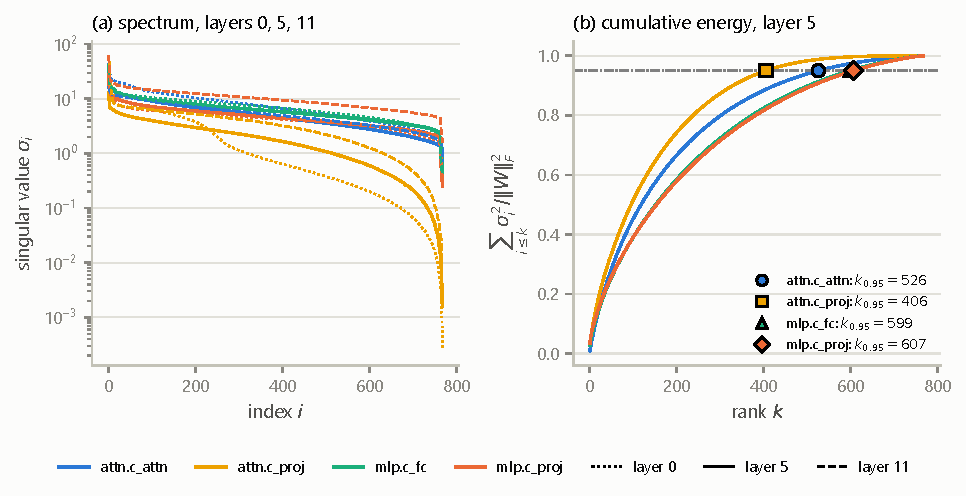
\includegraphics[width=0.72\textwidth]{figures/fig1_spectrum_energy.pdf}
\caption{(a) Singular values of the matrices in layers 0, 5 and 11 (log scale): after the first few they are nearly flat, so no small set of directions dominates. (b) Fraction of the energy kept by the best rank-$k$ approximation in layer 5; markers show the ranks that keep 95\% (406--607), all close to $\kbe$.}
\label{fig:spectrum}
\end{figure}

\paragraph{How low rank are the weights? Not very.}
A matrix compresses well if a few singular values are large and the rest small (fast \emph{decay}). GPT-2's singular values fall quickly for the first few and then stay nearly flat (Figure~\ref{fig:spectrum}(a)), so the energy is spread over hundreds of directions and keeping 95\% of it needs a rank close to break-even (panel (b)). In layer 5, $k_{0.95}/\kbe=0.913$--$1.057$ (Table~\ref{tab:dense}). Over all 48 matrices it is $0.53$--$1.20$, and 13 matrices need more than $\kbe$ (Figure~\ref{fig:breakeven}): for those, the factored version that keeps 95\% of the energy would be \emph{larger} than the original. Only four matrices are clearly below the line ($k_{0.95}/\kbe<0.9$): \mtx{attn.c\_proj} and \mtx{attn.c\_attn} in layers 0 and 1 ($0.53$--$0.87$). At a useful compression such as $k=32$, even the best possible approximation has relative error $0.72$--$0.93$ ($0.866$--$0.899$ in layer 5); it misses most of the matrix.

\begin{figure}[!tb]
\centering
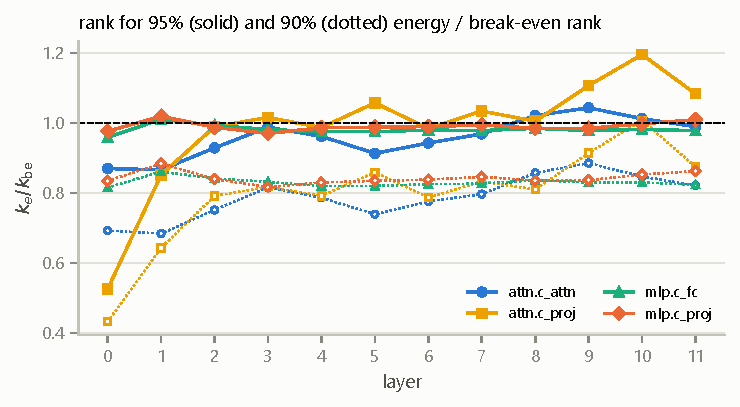
\includegraphics[width=0.55\textwidth]{figures/fig4_rank_vs_breakeven.pdf}
\caption{Rank needed for 95\% (solid) and 90\% (dotted) of the energy, divided by $\kbe$, for all 48 matrices. Above the dashed line the factored layer would be larger than the dense one.}
\label{fig:breakeven}
\end{figure}

\begin{table}[!tb]
\centering\small
\setlength{\tabcolsep}{3pt}
\begin{tabular*}{\textwidth}{@{\extracolsep{\fill}}l *{9}{r}@{}}
\toprule
 & & & & & \multicolumn{3}{c}{error ratio} & \multicolumn{2}{c}{speedup}\\
\cmidrule(lr){6-8}\cmidrule(l){9-10}
matrix (layer 5) & $\kbe$ & $k_{0.95}$ & $k_{0.95}/\kbe$ & $\epsEY(32)$ & $q=0$ & $q=1$ & $q=2$ & $q=0$ & $q=2$\\
\midrule
\mtx{attn.c\_attn} & 576 & 526 & 0.913 & 0.893 & 1.062 & 1.022 & 1.009 & 10.9 & 5.3\\
\mtx{attn.c\_proj} & 384 & 406 & 1.057 & 0.866 & 1.073 & 1.024 & 1.010 & 19.6 & 8.3\\
\mtx{mlp.c\_fc} & 614.4 & 599 & 0.975 & 0.899 & 1.058 & 1.020 & 1.008 & 24.0 & 14.1\\
\mtx{mlp.c\_proj} & 614.4 & 607 & 0.988 & 0.896 & 1.059 & 1.019 & 1.008 & 22.0 & 7.1\\
\bottomrule
\end{tabular*}
\caption{Regime A, layer 5. $k_{0.95}$ is the rank that keeps 95\% of the energy; $k_{0.95}/\kbe>1$ means the factored layer would be larger than the original. $\epsEY(32)$ is the best possible relative error at rank 32. The error ratio (RSVD error divided by the best possible error; median of 5 draws, $p=10$) and the speedup over the exact SVD are at $k=32$, for $q$ power iterations.}
\label{tab:dense}
\end{table}

\begin{figure}[!tb]
\centering
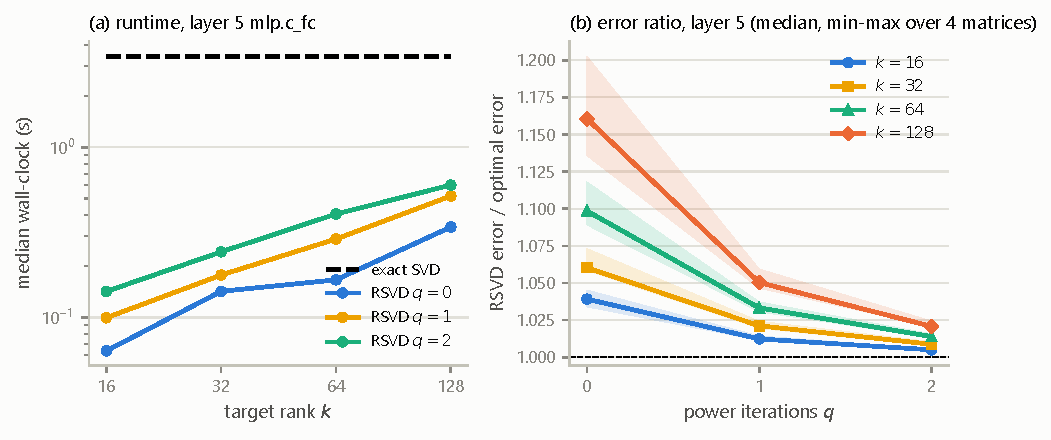
\includegraphics[width=0.75\textwidth]{figures/fig2_rsvd_vs_svd.pdf}
\caption{(a) Run time of RSVD for \mtx{L5.mlp.c\_fc} (layer 5) at each rank; the exact SVD is the dashed line. (b) RSVD error divided by the best possible error, over the four layer-5 matrices (line: median; band: min to max). One power iteration ($q=1$) removes most of the gap.}
\label{fig:rsvd}
\end{figure}

\paragraph{How good is RSVD? Fast and nearly optimal.}
In layer 5, RSVD was $2.9$--$53.8\times$ faster than the exact SVD (Figure~\ref{fig:rsvd}(a)). Its error was close to optimal, and one power iteration removed most of the remaining gap (panel (b)): the error ratio is $1.058$--$1.073$ without power iterations and $1.008$--$1.010$ with two at $k=32$ (Table~\ref{tab:dense}). Over all 48 matrices and the four ranks, the error ratio (each a median of 5 draws) lies between $1.02$ and $1.33$ at $q=0$ and between $1.003$ and $1.030$ at $q=2$; it grows with the rank, with medians over the matrices of $1.04$ ($k=16$) to $1.14$ ($k=128$) at $q=0$ and $1.005$ to $1.02$ at $q=2$. Power iterations cost time, so the speedup at $q=2$ is smaller.

\paragraph{Do the theoretical bounds help? No.}
The bound of Theorem~\ref{thm:exp} on the average squared error is at least $1.67\fro W^2$ in all 192 cases, while any projection has squared error at most $\fro W^2$ (the error of approximating $W$ by zero). So the bound, and Corollary~\ref{cor:epsdelta} built on it, is true but says nothing useful here. The measured squared error was only $1.03$--$1.71\times$ the optimum $\fro{W-W_k}^2$. The bounds are designed for fast-decaying spectra, and GPT-2's is flat.

\means GPT-2's weight matrices are far from low rank: a factorization saves memory only at a large error. RSVD computes it quickly and almost optimally, but its proven bounds are useless on such flat spectra. (Times are float64 CPU medians on a laptop that was shared with other jobs during this run; an idle-CPU rerun gave $3.4$--$63.1\times$, see Appendix~\ref{app:rerun}.)

\subsection{Regime B: can ALS fill in deleted weights?}
\label{sec:masked}

\begin{figure}[!tb]
\centering
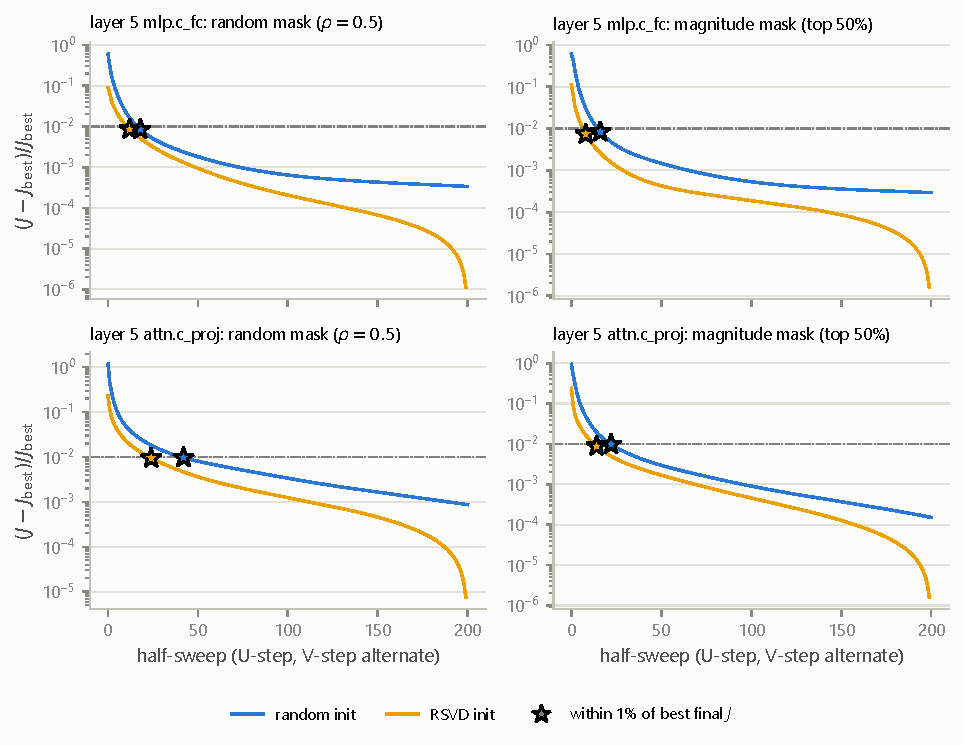
\includegraphics[width=0.7\textwidth]{figures/fig3_als_convergence.pdf}
\caption{ALS on two layer-5 matrices: how far $J$ is above the best final value, $(J-J_{\mathrm{best}})/J_{\mathrm{best}}$ (log scale; lower is better). The $x$-axis counts \emph{half}-sweeps, so a star at $2s$ means $s$ sweeps to get within 1\%. $J_{\mathrm{best}}$ is the RSVD-start run's own final value, so that curve drops to zero at the end by construction.}
\label{fig:als}
\end{figure}

\paragraph{Does ALS behave as the theory says? Yes.}
$J$ decreased at every half-step in all runs, as Theorem~\ref{thm:mono} promises. Starting from RSVD gets within 1\% of the best final $J$ about twice as fast as a random start ($4$--$12$ sweeps instead of $8$--$21$; Figure~\ref{fig:als}, Table~\ref{tab:masked}). After 100 sweeps both starts have essentially stopped moving, and their final values differ by only $0.015$--$0.087\%$.

\begin{table}[!tb]
\centering\small
\begin{tabular*}{\textwidth}{@{\extracolsep{\fill}}l l *{7}{r}@{}}
\toprule
 & & \multicolumn{2}{c}{sweeps to $1\%$} & \multicolumn{2}{c}{final $J$} & \multicolumn{2}{c}{ALS (RSVD start)} & zero-fill\\
\cmidrule(lr){3-4}\cmidrule(lr){5-6}\cmidrule(lr){7-8}\cmidrule(lr){9-9}
matrix (layer 5) & mask & random & RSVD & random & RSVD & known & held-out & held-out\\
\midrule
\mtx{mlp.c\_fc} & random & 9 & 6 & 14230.9 & 14226.1 & 0.867 & 1.015 & 0.989\\
\mtx{mlp.c\_fc} & magnitude & 8 & 4 & 24462.4 & 24455.2 & 0.831 & 2.231 & 1.289\\
\mtx{attn.c\_proj} & random & 21 & 12 & 1643.46 & 1642.03 & 0.794 & 1.723 & 1.009\\
\mtx{attn.c\_proj} & magnitude & 11 & 7 & 2989.73 & 2989.28 & 0.784 & 2.810 & 1.338\\
\bottomrule
\end{tabular*}
\caption{Regime B: $k=32$, half the entries known, 100 sweeps. ``Sweeps to 1\%'': sweeps until $J$ is within 1\% of the best final value, from a random or an RSVD start. ``Known'': relative error on the known entries. ``Held-out'': relative error on the hidden entries; 1 is what predicting 0 everywhere gives, so values $\ge1$ mean no predictive power. ``Zero-fill'': a rank-32 RSVD of the matrix with the hidden entries set to 0.}
\label{tab:masked}
\end{table}

\paragraph{Can ALS predict the hidden weights? No.}
On the \emph{known} entries ALS fits better than zero-filled RSVD (relative error $0.784$--$0.867$ vs.\ $0.853$--$0.924$). On the \emph{hidden} entries, started from RSVD, it scores $1.015$--$1.723$ with the random mask and $2.231$--$2.810$ with the magnitude mask (Table~\ref{tab:masked}; the random start gives similar values): no better than predicting zero, and worse than plain zero-filling. The closer ALS fits the known half, the worse it predicts the other half; this is overfitting. Tuning does not fix it: a grid over $k\in\{8,32,128\}$ and $\rho\in\{0.3,0.5,0.8\}$ on one matrix (Table~\ref{tab:grid} in Appendix~\ref{app:extra}) gives a held-out error of $1.61$--$2.14$ everywhere, while an ``oracle'' rank-$k$ fit computed from the \emph{full} matrix would score $0.64$--$0.95$ on the hidden entries.

\means The algorithm works as proved; the data do not cooperate. Filling in missing entries from known ones (\emph{matrix completion}) works only when the matrix is close to low rank \cite{jain2013}, and Regime A showed that GPT-2's weights are not. Pruned weights cannot be recovered by a low-rank model.

\subsection{Regime C: model quality and speed}
\label{sec:quality}

Regimes A and B judge an approximation by its \emph{weight error} $\fro{W-\hat W}/\fro W$. Regime C asks directly whether the compressed model still works (\texttt{experiments/model\_quality.py}). All 48 matrices are replaced at the same time by factors $U$, $V$, and each layer computes $(xU)V\T+b$; the embeddings and the output layer stay dense. Factors are computed in float64 and the model runs in float32 on the CPU (4 threads, i.e.\ 4 processor cores working in parallel). Every matrix gets the same parameter ratio $r\in\{0.9,0.7,0.5\}$, i.e.\ rank $k=\lfloor r\kbe\rfloor$, which is $192$--$552$ depending on the shape. We also try the energy rule of Regime A: each matrix gets the rank that keeps 95\% (or 99\%) of its energy, and a matrix whose rank would reach $\kbe$ is left dense.

\paragraph{Activation-aware SVD.}
A layer is only ever applied to real inputs, so the error that matters is in its outputs: $\fro{X(W-\hat W)}$, where the rows of $X$ are the layer's inputs on calibration text. We form $C=X\T X/N$ ($N$ tokens) and factor $C=LL\T$ with a lower-triangular $L$ (the \emph{Cholesky factorization}, after adding $10^{-4}$ times the mean diagonal of $C$ for numerical safety). Then
\[
\fro{X(W-\hat W)}^2=N\,\fro{L\T(W-\hat W)}^2 ,
\]
exactly for $LL\T=C$ (with the small ridge it holds for $C$ plus the ridge, a negligible change). Since $L$ is invertible, Eckart--Young (Theorem~\ref{thm:ey}) applied to $L\T W$ gives the best rank-$k$ choice $\hat W=L^{-\mathsf T}[L\T W]_k$, where $[\cdot]_k$ is the truncated SVD. This is the idea behind SVD-LLM \cite{wang2025svdllm} and ASVD \cite{yuan2023asvd}, without their further refinements. The \emph{activation-aware RSVD} variant computes $[L\T W]_k$ with RSVD ($q=2$). The \emph{output error} is $\fro{X(W-\hat W)}/\fro{XW}$, measured on the test text.

\plain Directions that the inputs rarely point in hardly affect the output. The method spends its limited rank on the directions the inputs actually use, and gives up accuracy in directions that never matter.

\begin{figure}[!tb]
\centering
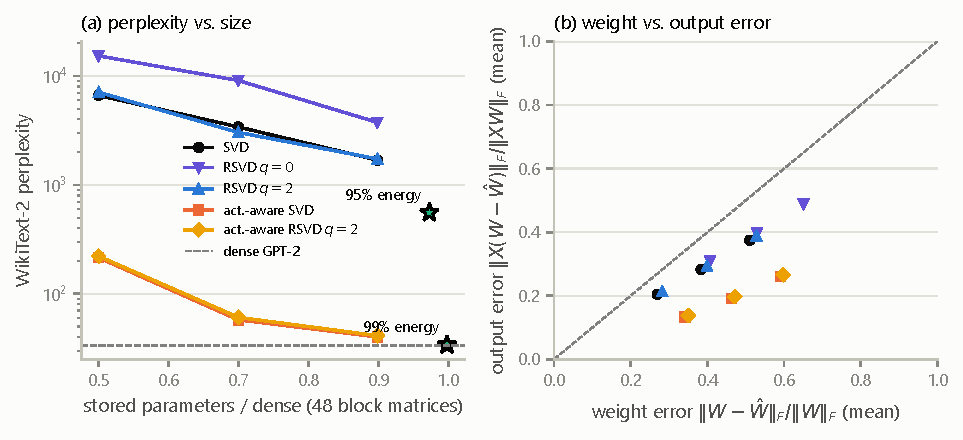
\includegraphics[width=0.82\textwidth]{figures/fig5_perplexity.pdf}
\caption{(a) WikiText-2 perplexity (log scale; dense GPT-2: $33.64$) against stored size for each method, after factorizing all 48 matrices at the same parameter ratio; stars mark the energy rule. Plain SVD and RSVD ($p=10$, one random draw) lose almost all predictive ability even at 90\% of the size; the activation-aware versions stay close to the dense model. (b) Weight error $\fro{W-\hat W}/\fro W$ against output error $\fro{X(W-\hat W)}/\fro{XW}$, both averaged over the 48 matrices, for the 15 runs of (a). Activation-aware factors have \emph{larger} weight error but much smaller output error.}
\label{fig:quality}
\end{figure}

\paragraph{Plain factorization breaks the model; activation-aware SVD keeps most of the quality.}
With the best possible rank-$k$ weights (plain SVD), keeping 90\%, 70\% and 50\% of the parameters raises perplexity from $33.6$ to $1689$, $3406$ and $6640$ (Figure~\ref{fig:quality}(a)); the model is effectively broken. This matches Regime A: at these ranks each matrix loses $7$--$37\%$ of its weight norm (mean $27\%$), and the errors of 48 layers add up. At the same sizes the activation-aware SVD gives perplexity $40.1$, $57.6$ and $214.4$, i.e.\ $1.19$, $1.71$ and $6.4$ times the dense model. Its weight error is \emph{higher} than plain SVD's ($0.342$ vs.\ $0.269$ at 90\%), but its output error is lower ($0.133$ vs.\ $0.205$).

\paragraph{Output error tracks perplexity better than weight error, but not perfectly.}
For plain SVD and RSVD the output error is about $0.73$--$0.76$ times the weight error, so the two move together (Figure~\ref{fig:quality}(b)). For the activation-aware methods it is $0.39$--$0.45$ times, so the same weight error does far less damage. Over all 15 runs the Spearman rank correlation with perplexity is $0.97$ for the output error and only $0.43$ for the weight error. Pooling the three sizes mixes two effects, though, because a smaller model has both larger errors and a higher perplexity. Within each size (5 methods each) the output error orders the methods almost exactly like perplexity (Spearman $1.00$, $0.90$ and $1.00$ at 90, 70 and 50\%), and the weight error does not ($0.20$, $0.10$, $0.20$). Across sizes the output error fails: plain SVD at 90\% has a \emph{smaller} output error than the activation-aware SVD at 50\% ($0.205$ vs.\ $0.260$) and a far higher perplexity ($1689$ vs.\ $214$). So weight error is a misleading criterion, and output error is a better but imperfect one; with 5 runs per size these correlations are rough.

\paragraph{Is RSVD good enough? With two power iterations, yes.}
Activation-aware RSVD ($q=2$) gives $41.2$, $60.7$ and $221.1$, within $2.6$--$5.3\%$ of the exact activation-aware SVD. Without power iterations, RSVD is much worse here than in Regime A: its mean weight error is $1.27$--$1.51$ times plain SVD's and its perplexity $2.2$--$2.7$ times. The reason is the rank: here $k$ is $192$--$552$ (Regime A used $k\le128$), the spectrum is flat, and $p=10$ extra vectors are too few to separate the top $k$ directions from the next ones. Power iterations fix this (Remark~\ref{rem:power}).

\paragraph{The energy rule gives almost no compression.}
At 95\% energy the same 13 matrices as in Regime A stay dense, the model keeps $97.3\%$ of the parameters, and perplexity is $556.1$. At 99\% energy only \mtx{L0.attn.c\_proj} is factored ($99.8\%$ of the parameters) and perplexity is $33.88$, essentially the dense value. Every factored matrix met the error guarantee of Proposition~\ref{prop:energy} ($\sqrt{1-0.95}=0.224$ and $\sqrt{1-0.99}=0.100$).

\begin{figure}[!tb]
\centering
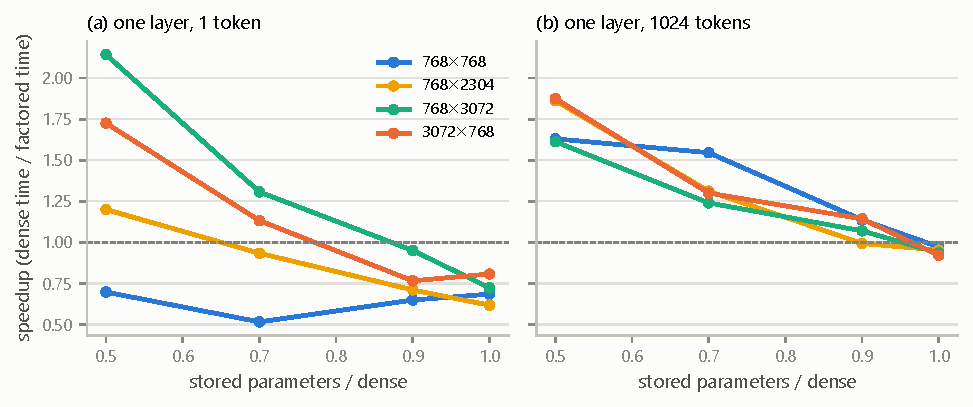
\includegraphics[width=0.76\textwidth]{figures/fig6_latency.pdf}
\caption{Speedup of one factored layer, $(xU)V\T$, over the dense layer $xW$ (above 1 = faster), in float32 on the CPU (median of 200 runs for 1 token, 20 runs for 1024 tokens), for the four matrix shapes, against the parameter ratio. At ratio 1 (rank $\approx\kbe$) both do the same arithmetic, and the factored layer is slower because it makes two calls instead of one.}
\label{fig:latency}
\end{figure}

\paragraph{Is the factored model faster? Only when it is much smaller.}
Figure~\ref{fig:latency} shows the \emph{speedup} (dense run time divided by factored run time) of one layer. At the break-even rank the factored layer is slower: $0.62$--$0.81\times$ for one token and $0.92$--$0.97\times$ for 1024 tokens. At 50\% of the parameters it is $1.61$--$1.88\times$ faster on 1024 tokens, and $1.20$--$2.14\times$ on one token for the three larger shapes. The small $768\times768$ layer is never faster on one token ($0.52$--$0.70\times$): it takes only $0.03$\,ms, so the fixed cost of each call dominates. For whole-model text generation (32-token prompt, 64 new tokens, activation-aware factors) the dense model takes $35.8$\,ms per token, and the factored model is $1.00\times$, $1.09\times$ and $1.27\times$ as fast at 90\%, 70\% and 50\% of the parameters. The gain is smaller than for one layer because the output layer ($768\times50257$), attention and the other operations are not compressed.

\paragraph{Caveats.}
Perplexity uses $8192$ tokens, RSVD one random draw, and there is no retraining after compression. Published methods such as SVD-LLM add further steps, so our activation-aware numbers are a basic version and are not comparable with their published results. The one-token timings are not reproducible (Appendix~\ref{app:rerun}).

\means Factorizing GPT-2's weights by the textbook criterion (smallest weight error) breaks the model; choosing the factors by the error on real inputs keeps it usable. Even so, a real saving (half the parameters, $1.27\times$ faster generation) still costs a large loss in quality. The lasting lesson, which the rest of the report applies to the KV cache, is to \emph{measure and minimize the error on the inputs a layer actually sees}, not the error in the stored numbers. This lesson is known in the literature \cite{hsu2022,wang2025svdllm,yuan2023asvd}; our comparison supports it on GPT-2 within each size, with the caveat that the output error alone does not compare models of different sizes.

% =====================================================================

% ---- end short/s04_weights ----
% ---- begin short/s05_kvlowrank ----
\section{Is the KV cache low rank?}
\label{sec:kv}
% =====================================================================

The weights are not low rank, so we turned to the KV cache, the larger memory cost at long contexts (Section~\ref{sec:kvcache}). This section asks whether GPT-2's cached keys and values are close to low rank, and whether a low-rank cache should use one basis per head, per layer or per group of heads. It ends with two questions that turned out to matter: the first token of each text, and the speed of a compressed cache.

\subsection{Related work on low-rank KV caches}
\label{sec:relwork}

We ran the experiments of Sections~\ref{sec:kv}--\ref{sec:kvupdate} first and checked the literature afterwards, so several of our designs were reached independently of, and later than, published ones. Palu \cite{palu2025} compares a basis per head, per group of heads and per layer; the per-layer basis is the most accurate but costs most at decoding, and Palu adopts groups as a compromise, as Sections~\ref{sec:option2}--\ref{sec:groups} also suggest for GPT-2. Query-aware keys (Section~\ref{sec:recipe}) are used by AttSVD \cite{attsvd2026} and SAKI \cite{saki2026}; KQ-SVD \cite{kqsvd2025} gives the closed-form optimal low-rank factorization of the attention score matrix (we did not check whether it also weights the values by $W_O$, as our output-aware values do). AttSVD builds its basis per prompt without calibration data and keeps the newest tokens exact. iS-KV \cite{iskv2026} is very close to our Section~\ref{sec:kvupdate}: a prompt basis shared by all heads of a layer, the last 128 tokens exact, and Brand's incremental SVD in blocks of 64 tokens, on 8-billion-parameter models. OjaKV \cite{ojakv2025} updates a calibration basis with Oja's rule \cite{oja1982}, a classical streaming rule that nudges a basis toward each new vector. The recipe of Sections~\ref{sec:kvonline} and~\ref{sec:kvupdate} is therefore not new. Related designs use offline low-rank attention \cite{saxena2024eigen}, low-rank keys for throughput \cite{sun2024shadowkv}, a subspace shared across layers \cite{chang2025xkv} (untested here), merged layers \cite{liu2024minicache}, low-rank key and value weights \cite{zhang2024lorc}, conversion to latent attention \cite{deepseek2024} with a short fine-tune \cite{ji2025mha2mla,meng2025transmla} (we do no training), or token sampling with subspaces \cite{s4r2026}.

Keeping the first tokens exact is common \cite{xiao2024sinks,ojakv2025}. SAKI reports, empirically, that low-rank key indexes can lose the attention-sink token unless it is kept exact \cite{saki2026}; it does not involve the geometry of Section~\ref{sec:sink}. ReadKV \cite{readkv2026} and AnchorKV \cite{anchorkv2026} also control the attention-output error; in the parts of these papers we read we did not find the sharp factor $\tfrac12$ of Lemma~\ref{lem:softmax} or the two-sided form of Lemma~\ref{lem:softmax2}. What we did not find elsewhere are the five analyses listed in Section~\ref{sec:intro}. All our results come from one small model without RoPE, with quality measured by perplexity only; the closest papers (iS-KV, AttSVD) use 8B-scale models with RoPE and task benchmarks.

\subsection{A first test: is each head's cache low rank?}
\label{sec:kvtest}

For a text of $T$ tokens, each head of each layer stores a key matrix $K$ and a value matrix $V$, both $T\times64$, one row per token. GPT-2 has no RoPE, so the cached keys are exactly the outputs of \mtx{attn.c\_attn}. The rule, fixed in advance: \emph{go} if in most layers (more than 6 of 12) the median head needs a rank below half its dimension, 32 of 64, to keep 95\% of the energy (Proposition~\ref{prop:energy}; script \texttt{experiments/kv\_spectra.py}, data of Section~\ref{sec:measure}, averaged over the 8 test windows). We also build a \emph{fixed basis} per head: the top $r$ right singular vectors of the calibration keys (or values), the columns of a $64\times r$ matrix $P$. (A \emph{basis} is a set of $r$ orthonormal directions; storing a vector ``in the basis'' means storing its $r$ coordinates along them. A real system would compute it once, offline.) Inside the model, every key $k$ (and/or value) is replaced by its projection $kPP\T$, so the cache keeps only the $r$ numbers $kP$ per token and head instead of 64.

\begin{figure}[!tb]
\centering
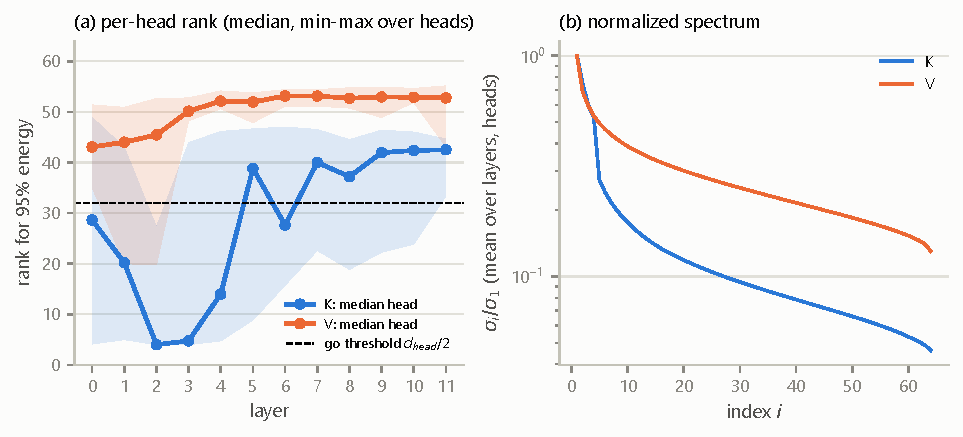
\includegraphics[width=0.7\textwidth]{figures/fig7_kv_spectra.pdf}
\caption{(a) Rank that keeps 95\% of the energy of each head's keys (blue) and values (orange), by layer: line = median head, band = range over the 12 heads. Below the dashed line (32) is ``go''. (b) Singular values divided by the largest, averaged over all layers and heads. Keys fall quickly after the first four; values decay slowly.}
\label{fig:kvspec}
\end{figure}

\paragraph{Verdict: no-go by our rule.}
For the keys, the median head is below 32 in 6 of 12 layers (layers 0--4 and 6), one short of ``most''; 49\% of all heads are below 32. For the values, no layer is below 32 and only 1.4\% of heads are (Figure~\ref{fig:kvspec}(a)). The median head needs $33.7$ of 64 dimensions for its keys and $52.1$ for its values ($36.5$ and $52.8$ after subtracting each head's mean). The keys are very uneven: about 4 dimensions in layers 2 and 3, 37--43 in layers 5 and 7--11, so one rank for all layers is the wrong design for keys. The values are uniformly hard (43--53 in every layer). A basis computed on the training text carries over to new text: it captures a median of $92.6\%$ of the test key energy at $r=32$ (worst head $81\%$) and $97.2\%$ at $r=48$; for values $73.8\%$ and $89.2\%$. So the low-rank structure belongs to the model, not to a particular text.

\begin{figure}[!tb]
\centering
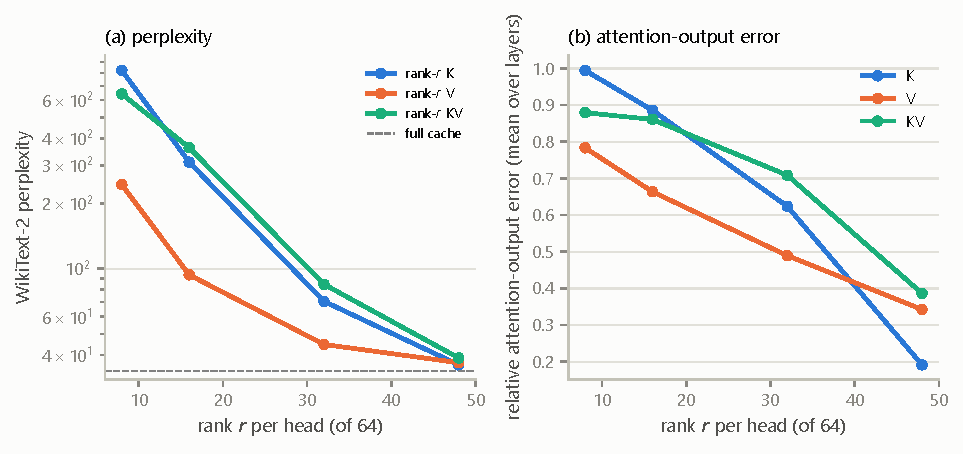
\includegraphics[width=0.64\textwidth]{figures/fig8_kv_perplexity.pdf}
\caption{(a) Perplexity (log scale) when the keys, the values, or both are stored at rank $r$ per head in every layer. (b) Relative change of the attention output, averaged over layers. Both fall steeply between $r=32$ and $r=48$.}
\label{fig:kvppl}
\end{figure}

\paragraph{Effect on the model.}
Figure~\ref{fig:kvppl} shows perplexity with a rank-$r$ cache (full cache $33.64$). At $r=8,16,32,48$ it is $825.5$, $310.7$, $70.6$, $35.9$ with only the keys compressed, $244.5$, $93.6$, $44.6$, $36.7$ with only the values, and $642.5$, $362.8$, $84.7$, $38.6$ with both. Keys at $r=48$ cost only $6.7\%$ in perplexity but save only $12.5\%$ of the cache (the values stay full); halving the cache (both at $r=32$) gives $84.7$. At low rank, key errors hurt \emph{more} than value errors, although keys hold their energy in fewer directions: through the softmax, a small key change alters \emph{which} tokens are attended to. As with the weights, the energy kept is not a reliable guide to the damage; the error in what the layer computes is.

\paragraph{Joining the heads.}
If the 12 heads of a layer are stacked side by side into one $T\times768$ matrix, 95\% of the key energy needs a median rank of only $67$ (range $4$--$104$) out of 768, and of the value energy $211$ ($119$--$238$). Energy is dominated by the heads with the largest entries, though, so heads with little energy could be badly damaged; Section~\ref{sec:option2} tests this in perplexity.

\means Head by head, the cache is not low rank enough: the values need most of their 64 dimensions, and the keys are low rank only in the early layers. A per-head cache of half the size raises perplexity from $33.6$ to $84.7$.

\subsection{One recipe for a weighted low-rank cache}
\label{sec:recipe}

After the no-go we tested two ideas. \emph{Option~1}: one basis per head, but each head gets its own key rank. \emph{Option~2}: one basis per layer, shared by all 12 heads (the ``joined'' matrix above). A middle test shares a basis among a \emph{group} of heads (Section~\ref{sec:groups}). All use one recipe, which also underlies Sections~\ref{sec:kvonline}--\ref{sec:kvupdate} (script \texttt{experiments/kv\_adaptive.py}; its plain rank-32 per-head keys reproduce the $70.58$ of Section~\ref{sec:kvtest} exactly).

\paragraph{The recipe.}
Let $x$ be the cached part of one token: one head's key (64 numbers) or a whole layer's keys (768 numbers). From the calibration text we take its mean $\mu$ (the average over tokens), its \emph{covariance} $C=\E[(x-\mu)\T(x-\mu)]$ (how the vectors spread around the mean, direction by direction), and a symmetric positive definite \emph{weight} matrix $G$ that says which errors matter. We store $z=(x-\mu)G^{1/2}U_r$, which is $r$ numbers, and the model uses
\begin{equation}\label{eq:recipe}
\hat x=\mu+(x-\mu)\,G^{1/2}U_rU_r\T G^{-1/2},\qquad\text{where}\quad G^{1/2}CG^{1/2}=U\Lambda U\T
\end{equation}
is an eigendecomposition and $U_r$ holds the eigenvectors of the $r$ largest eigenvalues. ($G^{1/2}$ is the symmetric square root of $G$, the matrix whose square is $G$.) This is the best rank-$r$ choice for the \emph{weighted error} $\E\lVert(x-\hat x)G^{1/2}\rVert^2$: after the change of variables $y=(x-\mu)G^{1/2}$ it is Eckart--Young again, exactly like the activation-aware SVD of Section~\ref{sec:quality}. The weights are:
\begin{itemize}[leftmargin=2em,itemsep=1pt]
\item $G=I$: \emph{plain} if also $\mu=0$ (as in Section~\ref{sec:kvtest}), \emph{centered} otherwise. Centering stores the mean once, exactly, and spends the whole rank on the deviations $x-\mu$. The mean itself needs no rank: for keys it adds the same amount $q\cdot\mu$ to every score of a query, and the softmax ignores a common shift; for values it passes through to the output unchanged, because the attention weights sum to 1. So centering looks like a free gain. (Section~\ref{sec:sink} shows a catch.)
\item Keys, \emph{query-aware}: $G=\E[q\T q]$, the \emph{second moment} (average outer product) of the queries of the same head, or the block-diagonal matrix of all heads that share the basis (each head's block on the diagonal, zeros elsewhere). Then the weighted error is the mean squared error of the attention \emph{score} $q\cdot k$, if queries and keys are independent.
\item Values, \emph{output-aware}: $G=W_OW_O\T$, built from the output matrix \mtx{attn.c\_proj}. Then the weighted error equals each token's value error after the output projection, where the layer writes its result (the attention-output error also has terms that mix tokens). For one head this is exact. For one basis shared by the 12 heads of a layer it is exact only if all heads give a token the same attention weight, because each head mixes its own values with its own weights; otherwise the cross-head terms of $W_OW_O\T$ do not match the real error. A planned block-diagonal alternative (one $W_O^h{W_O^h}\T$ block per head; rule \rl{G1}, perplexities within $0.3\%$) fails: with the offline basis it is worse ($+3.4\%$ for values at $R=512$, $34.29\to35.46$; $+3.1\%$ for the half cache, $34.98\to36.07$), and with the updated basis and buffer of Section~\ref{sec:kvupdate} it is not worse ($24.778\to24.762$, ratio $0.9994$). So the full $W_OW_O\T$ stays.
\end{itemize}

\plain Before choosing which directions to keep, stretch the space so that directions in which an error would hurt attention become long and harmless directions become short. Then keep the strongest directions, as the SVD always does. This is the ``measure the error on what the layer computes'' lesson of Section~\ref{sec:quality}, applied to keys and values.

\paragraph{Ranks and the pass rule.}
With one basis per head, the ranks can be the same $r$ everywhere (\emph{uniform}); per head, the smallest $r$ that keeps a share $e$ of the energy (\emph{threshold}); set by keeping the largest eigenvalues $\Lambda$ over all heads and layers for a given total (\emph{greedy}); or greedy within each layer only, each layer getting the same total (\emph{in-layer}). The pass rule, fixed before the run, calls a cache ``close'' if its perplexity is at most 5\% above the full cache ($\le35.33$). Option~1 passes if the keys alone can be halved (average rank $\le32$ of 64) and stay close; Option~2 passes if keys and values together fit in half the cache and stay close.

\subsection{Option 1, a rank per head: fails}
\label{sec:option1}

\begin{figure}[!tb]
\centering
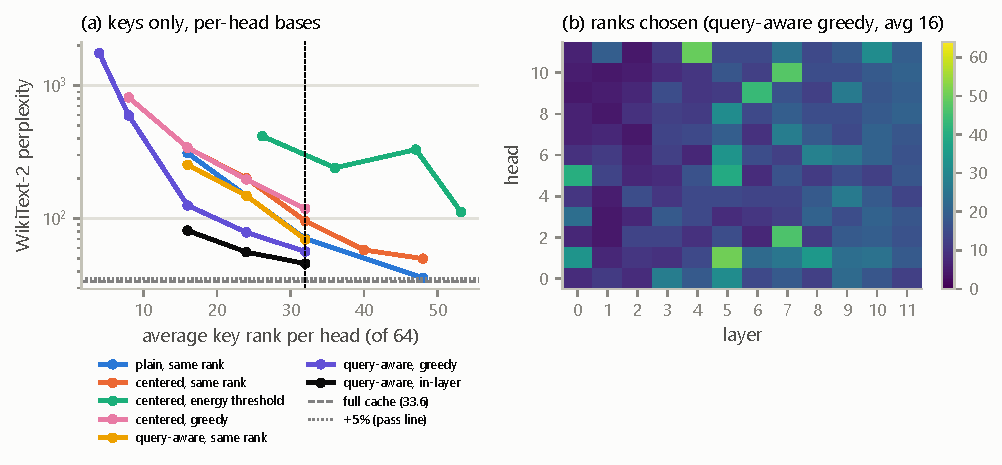
\includegraphics[width=0.7\textwidth]{figures/fig9_kv_perhead.pdf}
\caption{Option~1, keys only, one basis per head. (a) Perplexity (log scale) against the average key rank for each way of setting ranks; the dashed vertical line is ``keys halved'' (rank 32). No method reaches the dotted pass line at rank $\le32$. (b) Ranks chosen by the query-aware greedy rule at an average of 16, per layer and head: most rank goes to the middle and late layers, and some heads get almost none.}
\label{fig:kvperhead}
\end{figure}

With the keys halved, the best method (query-aware, in-layer ranks) reaches $45.8$ ($+36\%$; Figures~\ref{fig:kvperhead}(a) and~\ref{fig:short-kvfollow}): better than one rank everywhere ($70.6$), far from the pass line. Energy is a bad guide for keys: the threshold rule is not even monotone (95\% of each head's energy, average rank $36$, gives $241$; 98\%, rank $47$, gives $330$). Query weighting helps (query-aware greedy $56.4$ at rank 32), but moving rank across layers hurts: in-layer beats greedy ($45.8$ vs.\ $56.4$; for values at rank 32, $95$ vs.\ $641$, because greedy starves the early layers, panel (b)). Centering hurts per-head keys ($95.8$ vs.\ $70.6$ at rank 32), although the mean cannot change the softmax; Section~\ref{sec:sink} explains this.

\subsection{Option 2, one basis per layer: passes}
\label{sec:option2}

\begin{figure}[!tb]
\centering
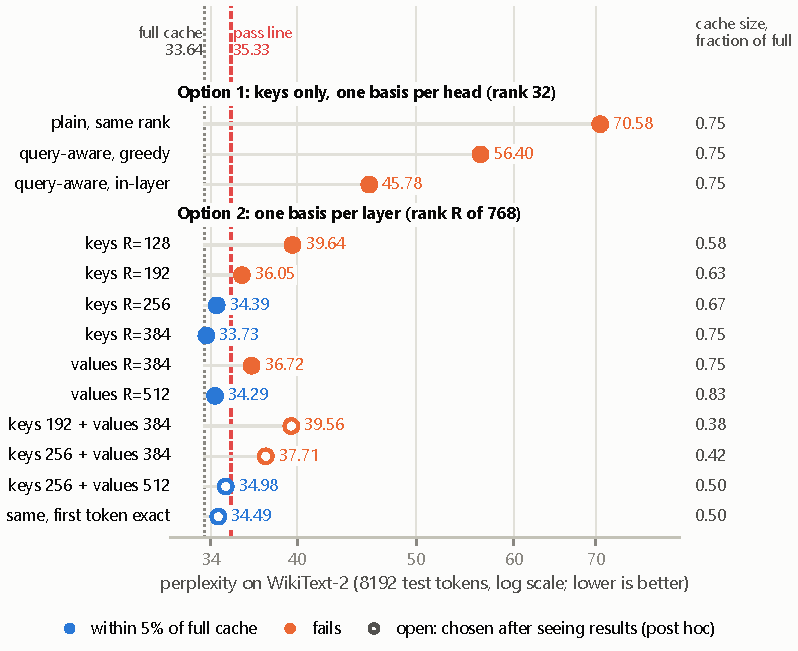
\includegraphics[width=0.9\textwidth]{figures/short_kvfollow.pdf}
\caption{Perplexity with a compressed KV cache (WikiText-2, 8192 test tokens; log scale). Blue: within 5\% of the full cache ($33.64$, dotted), i.e.\ below the pass line $35.33$ (dashed); orange: fails. Open rings: pairs added after the first pass (post hoc), chosen from the key-only and value-only rows; see the confirmation run in the text. The last row comes from the first-token test of Section~\ref{sec:sink}. Right column: size of the whole cache relative to the full cache. The compressed part alone keeps $R/768$ of its cache (keys at $R=256$: a third), or $32/64$ per head in Option~1, whose first row is the plain cache of Section~\ref{sec:kvtest}.}
\label{fig:short-kvfollow}
\end{figure}

\begin{figure}[!tb]
\centering
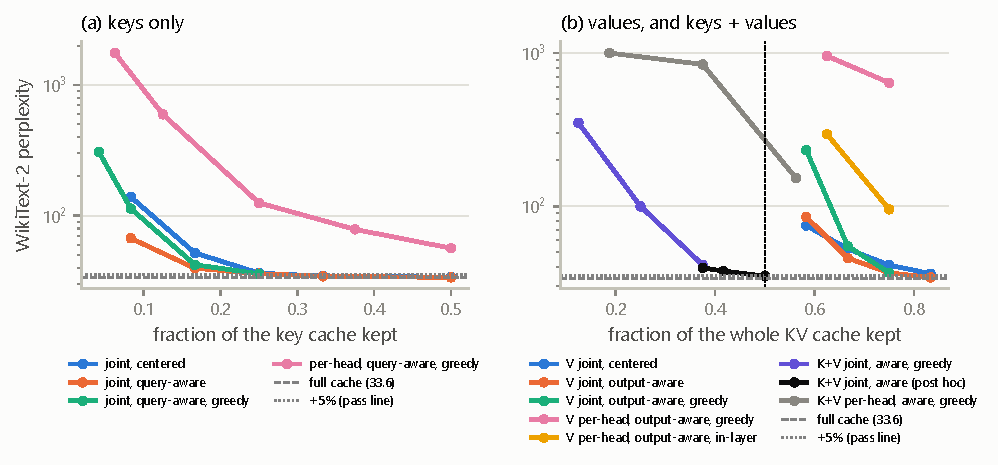
\includegraphics[width=0.72\textwidth]{figures/fig10_kv_joint.pdf}
\caption{Option~2, one basis per layer. (a) Keys only, perplexity against the share of the key cache kept; the per-head method of Figure~\ref{fig:kvperhead} is shown for comparison. (b) Values, and keys plus values, against the share of the whole cache kept; the dashed vertical line is half the cache. In the legends, ``joint'' means one basis per layer and ``per-head'' one basis per head; ``aware'' means query-aware keys with output-aware values.}
\label{fig:kvjoint}
\end{figure}

A basis shared by the 12 heads of a layer is far better than separate bases of the same total size (Figures~\ref{fig:short-kvfollow} and~\ref{fig:kvjoint}). For keys, $R=384$ stores as much as rank 32 per head ($12\times32=384$) and gives $33.73$ instead of $45.8$. Keeping a third of the key cache ($R=256$, whole cache $0.67$) gives $34.39$ ($+2.2\%$); $R=192$ ($36.05$) and $R=128$ ($39.64$) fail. Values need more: $R=512$ (whole cache $0.83$) gives $34.29$ ($+1.9\%$), $R=384$ ($36.72$) fails. Together, keys at $R=256$ and values at $R=512$ fill exactly half the cache at perplexity $34.98$ ($+4.0\%$), just inside the pass line ($34.49$ with the first token exact); the two smaller post hoc pairs fail ($39.56$ at $0.38$ and $37.71$ at $0.42$ of the cache). Query-aware and plain bases are close from $R=192$ up, and greedy allocation across layers helps little or hurts ($42.2$ vs.\ $39.6$ at $R=128$, $36.0$ vs.\ $36.1$ at $R=192$).

\paragraph{Confirmation on fresh text.}
The passing pair K256/V512 was chosen after seeing the other rows on the same test windows (post hoc), which could flatter it. On the next 8 test windows, which no run had used (full cache $28.22$), the half-size cache gives $29.31$ ($+3.9\%$), keys at $R=256$ alone $+2.3\%$, values at $R=512$ alone $+1.6\%$, and per-head in-layer keys at rank 32 $+34\%$: all within one percentage point of the first run.

\paragraph{The cost: more arithmetic.}
To score a query against the compressed keys, head $h$ computes $(q_hB_h)\cdot z$, where $B_h$ is the head's $64\times R$ block of the basis and $z$ the stored code: $R$ multiply-adds per cached token instead of 64, and similarly for values. At K256/V512, attention over the cache needs about $(256+512)/(64+64)=6\times$ the multiply-adds of the full cache, while reading half the memory. Decoding is usually limited by memory reads (Section~\ref{sec:cost}), so this could still be faster; Section~\ref{sec:timing} measures it.

\means A per-layer basis halves GPT-2's KV cache within the 5\% line, on fresh text too. The saving comes from directions that the heads of a layer have in common, and it is paid for in arithmetic.

\subsection{Groups of heads: no cheaper middle ground}
\label{sec:groups}

\begin{figure}[!tb]
\centering
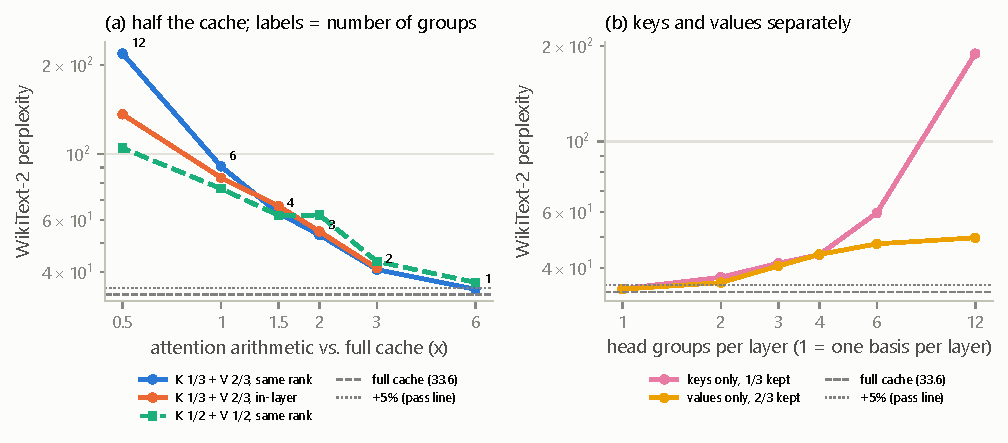
\includegraphics[width=0.7\textwidth]{figures/fig11_kv_groups.pdf}
\caption{Bases shared by groups of consecutive heads (full cache $33.64$, pass line $35.33$). (a) Half the cache: perplexity against the attention arithmetic. Each point is a number of groups (labels); fewer groups means more arithmetic and lower perplexity. (b) Keys only (a third kept) and values only (two thirds kept), against the number of groups.}
\label{fig:kvgroups}
\end{figure}

To cut the arithmetic we gave each of $g$ groups of consecutive heads ($g=1,2,3,4,6,12$) its own basis, with the same recipe and pass rule. At half the cache (keys $\tfrac13$, values $\tfrac23$ of the group width $768/g$) the arithmetic is $6/g$ times that of the full cache; $g=1$ reproduces $34.98$ exactly. \emph{Only one basis per layer passes} (Figure~\ref{fig:kvgroups}): at half the cache perplexity is $34.98$, $40.73$, $53.38$, $63.18$, $90.84$ and $218.13$ for $g=1,2,3,4,6,12$. Two groups ($3\times$ the arithmetic) already cost $+21\%$; at the full cache's arithmetic ($g=6$) the best variant gives $76.40$, and per head $104.78$ (both splitting the width evenly between keys and values). Keys suffer most from splitting (a third kept: $34.39$ at $g=1$, then $37.38$, $41.39$, $44.03$, $59.59$, $188.85$); values degrade gently ($34.29$ to $49.77$; two groups $35.96$, $+6.9\%$).

\means The saving needs directions shared across the whole layer: among the groupings tested, halving the cache at $+4\%$ needs the full $6\times$ arithmetic. We grouped consecutive heads only; grouping heads with similar subspaces might do better, untested.

\subsection{The first token: why removing the mean hurts per-head keys}
\label{sec:sink}

\begin{figure}[!tb]
\centering
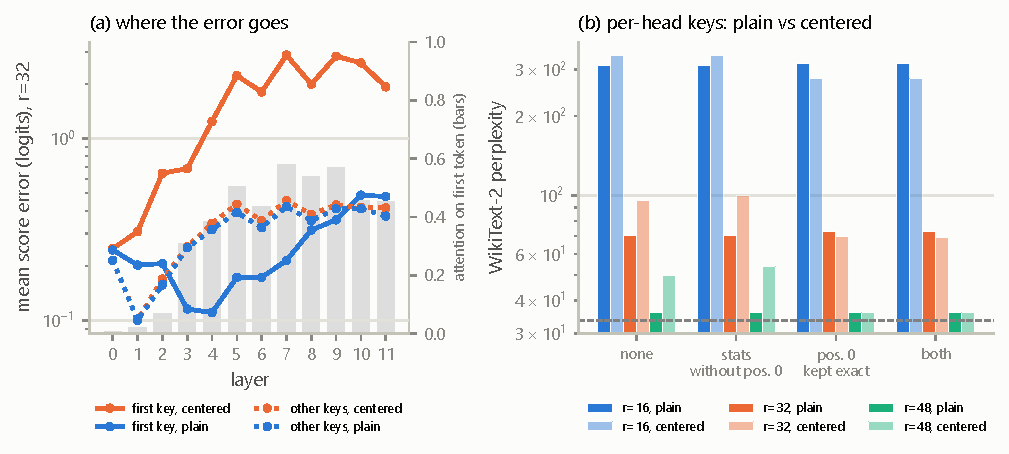
\includegraphics[width=0.74\textwidth]{figures/fig13_kv_sink.pdf}
\caption{Why centering hurts per-head keys. (a) Rank-32 per-head keys on two test windows only (\texttt{kv\_sink\_check.py} default): mean error in the attention score (in logits) for the first key of the window (solid) and for all other keys (dotted), median over heads, by layer. Grey bars: share of attention that queries put on the first token. (b) Perplexity of plain and centered per-head keys at ranks 16, 32, 48: unchanged, with the first token left out of the calibration statistics, with the first token's key stored exactly, or both. Dashed line: full cache.}
\label{fig:kvsink}
\end{figure}

Removing the mean before projecting should be harmless (Section~\ref{sec:recipe}), yet it made per-head keys much worse ($95.8$ vs.\ $70.6$ at rank 32). The cause is the first token. Language models put much of their attention on the first token of the text, whatever it is; this is called an \emph{attention sink} \cite{xiao2024sinks}. In GPT-2's layers 3--11, queries put $31$--$58\%$ of their attention on position 0 (median per layer; grey bars in Figure~\ref{fig:kvsink}(a)), so an error on that one key matters a great deal.

\paragraph{What is special about the first key.}
Not its size: the first token's keys are \emph{smaller} than typical keys ($0.24$--$0.73$ times the typical length) and contribute at most $1\%$ of the key variance, and leaving them out of the calibration statistics makes things slightly worse (centered, rank 32: $100.0$ instead of $95.8$). What is special is their \emph{direction}. Write $\hat\mu=\mu/\lVert\mu\rVert$ for the unit vector along the mean key. The first key's coordinate along it, $k_0\cdot\hat\mu$, is negative in all 12 layers: between $-0.21\lVert\mu\rVert$ and $-1.35\lVert\mu\rVert$ (median over heads, by layer; median of all heads $-0.40\lVert\mu\rVert$). So $k_0$ lies on the other side of the origin from the mean, and its deviation $k_0-\mu$ has a large component along $\hat\mu$, between $-1.21$ and $-2.35\lVert\mu\rVert$ (median $-1.40\lVert\mu\rVert$). A centered basis is computed from the deviations $k-\mu$ of all tokens, and for typical tokens these are not concentrated along $\hat\mu$. So the basis need not contain that direction, and the reconstruction $\mu+(k_0-\mu)P$ can lose most of the first key's deviation along $\hat\mu$, pulling $k_0$ back towards $\mu$. The plain basis has less of this problem, because its second moment $\E[k\T k]=C+\mu\T\mu$ (keys are row vectors) contains $\mu\T\mu$, which favours keeping the mean direction. Remark~\ref{rem:sink} turns this into a lower bound on the error; it is a consistent explanation, not a proof that it is the cause.

Figure~\ref{fig:kvsink}(a) shows the effect: at rank 32 the score error on the first key is $1.65$ logits for the centered basis against $0.22$ for the plain one (median over layers and heads), and up to $2.9$ in the middle layers, which changes that token's attention weight by a factor of up to $e^{2.9}\approx18$. On the other keys the two bases are about equal ($0.37$ vs.\ $0.33$). A rerun on 16 test windows confirms this (rule \rl{K2}, negative in at least 9 of 12 layers, passes): layer medians $-0.21$ to $-1.33\lVert\mu\rVert$ for $k_0\cdot\hat\mu$ (negative in all 12 layers, overall median $-0.40\lVert\mu\rVert$) and $-1.21$ to $-2.33\lVert\mu\rVert$ for $(k_0-\mu)\cdot\hat\mu$; first-key score errors $1.59$ logits centered vs.\ $0.22$ plain (other keys $0.36$ and $0.34$).

\begin{remark}[Error on the first key under a centered basis]\label{rem:sink}
Keys are row vectors. Let a centered per-head basis with $G=I$ reconstruct $\hat k_0=\mu+(k_0-\mu)P$, where $P=U_rU_r\T$ and $U_r$ has orthonormal columns. Write $k_0-\mu=c\,\hat\mu+w$, where $c=(k_0-\mu)\cdot\hat\mu$ is the deviation's coordinate along the mean direction and $w\perp\hat\mu$ is the rest. The reconstruction error is $\lVert k_0-\hat k_0\rVert=\lVert(c\hat\mu+w)(I-P)\rVert$, and the reverse triangle inequality gives
\[
\lVert k_0-\hat k_0\rVert\;\ge\;\lvert c\rvert\,\lVert\hat\mu(I-P)\rVert-\lVert w(I-P)\rVert .
\]
With a query-aware weight $G$ the same holds in weighted coordinates: the left side becomes $\lVert(k_0-\hat k_0)G^{1/2}\rVert$, $k_0-\mu$ is replaced by $(k_0-\mu)G^{1/2}$ and $\hat\mu$ by the unit vector along $\mu G^{1/2}$. Our numerical check uses $G=I$.
\end{remark}
\plain The error is large when $k_0$'s deviation along the mean, $\lvert c\rvert$ (here $1.21$--$2.35\lVert\mu\rVert$), is large and the basis misses the mean direction ($\lVert\hat\mu(I-P)\rVert$ close to 1), unless the rest of the deviation happens to cancel it. On 16 windows at rank 32, $\lVert\hat\mu(I-P)\rVert$ has a median of $0.45$ for the centered basis and $0.008$ for the plain one. The lower bound held in all 2304 cases (heads, layers and windows) and was positive, i.e.\ informative, in 1820 of them, because $\lvert c\rvert$ is large (median $9.7$ against $2.1$ for $\lVert w(I-P)\rVert$).

\paragraph{The test, with its rule fixed before the run.}
If the first token explains the gap, then under some treatment of it the centered keys should be no worse than the plain ones at ranks 16, 32 and 48. Storing the first token's key exactly (one token in 1024, so the cache size is unchanged to three decimals) does this (Figure~\ref{fig:kvsink}(b)): centered vs.\ plain gives $278$ vs.\ $317$, $70.0$ vs.\ $73.3$ and $35.89$ vs.\ $35.97$. Leaving it out of the statistics does not ($340$, $100$, $54$). On the fresh windows centered keys at rank 32 go from $76.0$ to $59.3$ with the first key exact, against $62.0$ for plain. Three caveats:
\begin{itemize}[leftmargin=2em,itemsep=1pt]
\item \emph{The fix makes the plain basis worse, and we cannot explain why.} Keeping the first key exact raises plain perplexity ($310.7\to317.3$ at rank 16, $70.58\to73.25$ at rank 32; fresh windows $59.04\to62.0$), so the rule passes partly because the comparison got worse. A later planned test (C20, a follow-up experiment named after its result file; see Section~\ref{sec:measure}) confirms this harm statistically only at rank 32, finds it almost entirely in layer 0, where position 0 gets almost no attention, and rejects the guess that the first key's error cancels the others' in the scores (Section~\ref{sec:kvadditive}). Nor does the sink lose attention: keeping the first key exact brings the attention on position 0 back towards the full model for both bases (rank 32, mean over layers: full $0.356$; plain $0.288\to0.301$; centered $0.205\to0.303$).
\item \emph{The margin at rank 48 is small} ($35.89$ vs.\ $35.97$, one run), and centered with the first key exact ($35.890$) is slightly \emph{worse} than plain with no treatment ($35.880$). The rule passes only against plain with the first key exact.
\item \emph{A planned alternative fix fails.} Adding the unit mean direction $\hat\mu$ to a centered basis of the same rank (rule \rl{K1}: no worse than plain at ranks 16, 32, 48) gives $317.6$, $72.34$ and $36.01$ against plain $310.7$, $70.58$ and $35.88$.
\end{itemize}
With the first key exact the best per-head method improves only from $45.8$ to $44.5$ (still fails); the passing per-layer setting improves from $34.98$ to $34.49$ ($+2.5\%$) with the first token's key and value exact (post hoc; fresh windows $29.06$, $+3.0\%$ against $+3.9\%$). All later sections keep the first token exact.

\means The results are consistent with geometry, not size: the sink token's key points away from the mean, so a basis that removes the mean can distort exactly the key that receives the most attention. Keeping that one token exact removes the gap at no measurable memory cost, subject to the three caveats above. The geometry is GPT-2's: on SmolLM2 the first key does not point away from the mean in most layers, although the sink still matters there and keeping position 0 exact helps every basis (C19, Section~\ref{sec:kvadditive}).

\subsection{Is the compressed cache faster? Not on a CPU}
\label{sec:timing}

\begin{figure}[!tb]
\centering
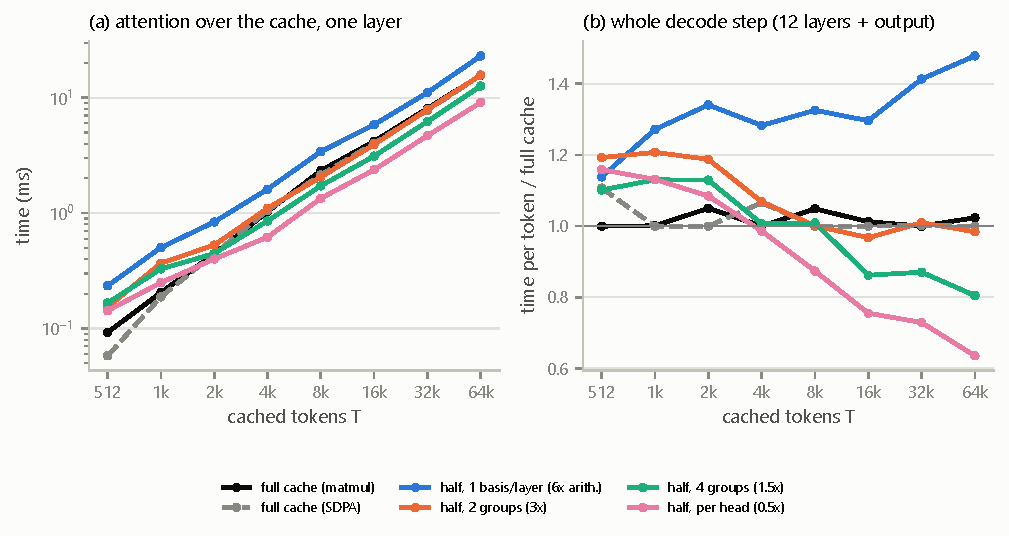
\includegraphics[width=0.74\textwidth]{figures/fig12_kv_timing.pdf}
\caption{CPU time to generate one token with $T$ tokens already cached (GPT-2 small shapes, float32, 4 threads, median of 12 rounds). (a) Attention over the cache in one layer. (b) The whole step (12 layers and the output layer), relative to the full cache (below 1 = faster). ``Half'' = half-size cache; the factor in brackets is the attention arithmetic. Lengths above 1024 exceed GPT-2's context and only measure the computation. The full cache is timed with plain matrix products (``matmul'') and with PyTorch's fused attention routine (``SDPA'', scaled dot-product attention); the reference in (b) is the faster of the two at each length. Against matmul alone at 65{,}536 tokens the ratios are $1.44$ (one basis per layer), $0.79$ (four groups) and $0.62$ (per head).}
\label{fig:kvtiming}
\end{figure}

We timed one generation step on the laptop's CPU with no other heavy job running (\texttt{experiments/kv\_timing.py}; recorded CPU load $0$--$17\%$ during the measurements, $24\%$ at the start). The factored computation agrees with attention on the reconstructed keys and values to $10^{-15}$. The question, fixed before the run: is one basis per layer no slower per token than the full cache once at least 4096 tokens are cached? \emph{No} (Figure~\ref{fig:kvtiming}): it costs $1.28$--$1.48\times$ the time of the faster full-cache variant per token for 4096--65{,}536 cached tokens (idle-CPU rerun $1.16$--$1.35\times$; Appendix~\ref{app:rerun}). That is far less than $6\times$, probably because it reads only half the memory and all 12 heads use each stored number (not measured separately). Per-head bases (half the arithmetic) are faster, $0.64\times$ at 65{,}536 tokens (attention itself $0.58\times$), four groups $0.81\times$, two groups $0.98\times$, but these fail on quality (Section~\ref{sec:groups}). At GPT-2's maximum of 1024 tokens every compressed variant is $13$--$27\%$ slower per token, from the fixed cost of encoding the new token and mapping the queries.

\paragraph{Why.}
A processor is limited either by arithmetic or by memory reads, depending on its operations per byte read (\emph{arithmetic intensity}). Full-cache attention reads about 25\,GB/s here at only $0.5$ floating-point operations (FLOP) per byte: memory-bound, which is why halving the cache per head nearly halves its time. The per-layer basis does about $6$ per byte, close to what this CPU sustains, so arithmetic decides. A GPU in 16-bit precision does about $100$ or more per byte, so there the per-layer basis should again be memory-bound and could be up to $2\times$ faster; we have not measured this. The timing applies to GPT-2's learned absolute positions only: with RoPE the score involves a rotation $R_{t-s}$ between query $t$ and the stored code of key $s$, so the key basis cannot be folded into the query once per step (values carry no rotation); with grouped-query attention the codes are shared among fewer key--value heads, so the factor differs from $6\times$.

\means On our CPU the half-size cache costs time instead of saving it. Whether it pays off on a GPU, where memory reads dominate, is the main open practical question for this design.

% =====================================================================

% ---- end short/s05_kvlowrank ----
% ---- begin short/s06_07_prompt_bounds ----
\section{A basis computed from the prompt}
\label{sec:kvonline}
% =====================================================================

So far every basis was computed once, \emph{offline}, from 16 windows of calibration text. This section computes it \emph{online}, from the text being processed, with the randomized SVD of Section~\ref{sec:rsvd}. This is where a fast factorization is needed, because it must run for every new input.

\paragraph{Setting.}
A model first reads the whole prompt at once (prefill) and then generates the continuation one token at a time (decode). We split each 1024-token test window into a \emph{prompt} of $P$ tokens, processed exactly, and a \emph{continuation}. In every layer a basis is then computed from the prompt's own keys and values; the whole cache (prompt and continuation) is stored in it, and the continuation runs on the compressed cache. Perplexity is measured on the continuation only (255 tokens per window, 16 windows, 4080 tokens at $P=768$). In Sections~\ref{sec:kvonline}--\ref{sec:kvupdate}, ``half (a third of) the cache'' means half (a third) of the numbers stored per token, the codes; the memory including the per-prompt basis is reported separately (Proposition~\ref{prop:kvmem}). Everything else is the passing recipe of Section~\ref{sec:option2} (one basis per layer, query-aware keys, output-aware values, mean removed, first token exact), with the mean and the query weight also taken from the prompt. The basis is the top $R$ right singular vectors of the weighted prompt matrix $A=(X-\mu)G^{1/2}$ (one row per prompt token, 768 columns), computed in three ways: from the calibration text as before (\emph{offline}); by an exact SVD of $A$ (\emph{online}); or by RSVD (Algorithm~\ref{alg:rsvd} applied to $A\T$, with oversampling $p=10$ and $q=0,1,2$ power iterations). A check: running the prompt and then the continuation with the full cache reproduces a single pass over the window (largest logit difference $0.0014$).

\begin{table}[!tb]
\centering\footnotesize
\setlength{\tabcolsep}{4pt}
\begin{tabular*}{\textwidth}{@{\extracolsep{\fill}}lcrrrrrr@{}}
\toprule
setting (codes kept) & memory & full cache & offline & online & RSVD $q{=}0$ & RSVD $q{=}1$ & RSVD $q{=}2$\\
\midrule
$P=768$, K 256 + V 512 (0.50) & 0.50 / 0.91 & 24.73 & 25.37 & 25.78 & 26.52 & 25.80 & 25.75\\
$P=768$, K 128 + V 384 (0.33) & 0.33 / 0.62 & 24.73 & 28.66 & 28.34 & 31.82 & 28.47 & 28.41\\
$P=384$, K 256 only (0.67) & 0.67 / 0.82 & 26.70 & 27.19 & 29.31 & -- & 29.37 & --\\
$P=512$, K 256 only (0.67) & 0.67 / 0.82 & 26.42 & 26.90 & 28.02 & -- & 28.01 & --\\
$P=768$, K 256 only (0.67) & 0.67 / 0.82 & 24.73 & 25.20 & 25.26 & -- & 25.33 & --\\
\bottomrule
\end{tabular*}
\caption{Perplexity on the continuation tokens (16 test windows). ``K 256 + V 512'' means keys stored at rank 256 and values at rank 512 of 768; ``codes kept'' is the share of numbers per token. ``Memory'': the whole cache at 1024 tokens relative to the full cache (Proposition~\ref{prop:kvmem}), for the offline basis / for the per-prompt bases (online and RSVD), which must store their own basis and key weight. ``Offline'': basis from calibration text; ``online'': exact SVD of the prompt; RSVD with $p=10$ and $q$ power iterations. The full-cache values differ between prompt lengths because they are measured on different tokens (the continuation is longer after a shorter prompt).}
\label{tab:kvonline}
\end{table}

\begin{figure}[!tb]
\centering
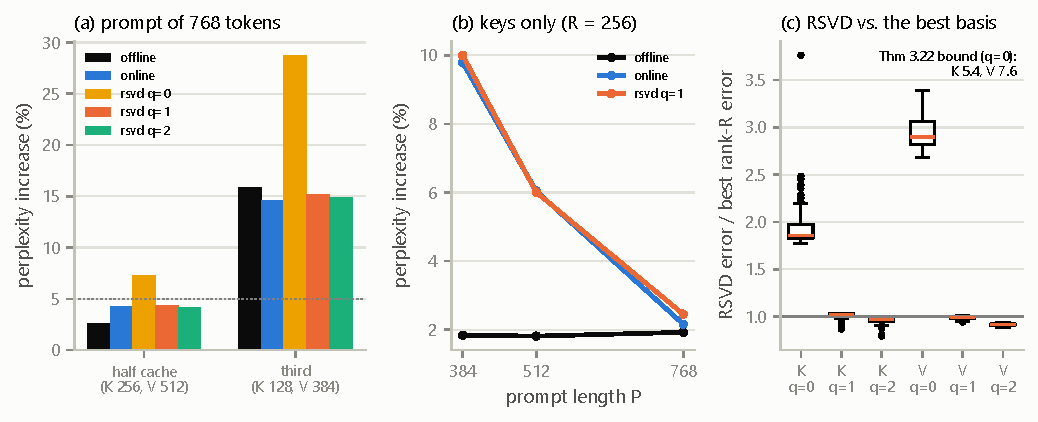
\includegraphics[width=0.9\textwidth]{figures/fig14_kv_online_fr.pdf}
\caption{Online basis. (a) Perplexity increase over the full cache with a 768-token prompt, at half and a third of the cache; dotted line: $+5\%$. (b) Keys only: how the online basis depends on the prompt length, compared with the offline basis. (c) RSVD error divided by the best possible rank-$R$ error, over all layers and windows (keys $R=256$, values $R=512$). The projection uses all $R+p$ columns of $Q$, so with power iterations its ratio can fall below 1. The bound of Theorem~\ref{thm:exp} on the average ($5.4$ for keys, $7.6$ for values) is far above every box.}
\label{fig:kvonline}
\end{figure}

\paragraph{Results} (Table~\ref{tab:kvonline}, Figure~\ref{fig:kvonline}). Three rules were fixed before the run, for a 768-token prompt at half the cache (keys $R=256$, values $R=512$; all rules are listed in Table~\ref{tab:rules}):
\begin{itemize}[leftmargin=2em,itemsep=1pt]
\item \emph{\rl{R1} (RSVD with one power iteration within $1\%$ of the exact online basis) passes.} With $q=1$ the perplexity is within $0.1\%$ of the exact SVD ($25.80$ vs.\ $25.78$), and $q=2$ is slightly better. Without power iterations RSVD is clearly worse ($26.52$, $+7.3\%$; at a third of the cache $+28.7\%$ instead of $+14.6\%$). As for the weights (Section~\ref{sec:quality}), the target rank is a large share of the dimension, the singular values beyond it are not small, and power iterations are needed (Remark~\ref{rem:power}).
\item \emph{\rl{R2} (online no worse than offline) fails}: $+4.2\%$ vs.\ $+2.6\%$ at half the cache. At a third of the cache online is slightly better ($+14.6\%$ vs.\ $+15.9\%$, both far from usable). The prompt must be long enough (Figure~\ref{fig:kvonline}(b)): for keys alone, the online basis costs $+9.8\%$, $+6.0\%$ and $+2.2\%$ after prompts of 384, 512 and 768 tokens, against about $+1.9\%$ for the offline basis at every length. A basis of 256 directions estimated from a few hundred tokens fits that prompt too closely; Section~\ref{sec:bound1} measures this.
\item \emph{\rl{R3} (RSVD with one power iteration within $5\%$ of the full cache) passes}: $+4.4\%$, with no calibration text at all.
\end{itemize}

\paragraph{Theory check and speed.}
Theorem~\ref{thm:exp} bounds the \emph{average} projection error by $\sqrt{1+R/(p-1)}$ times the best rank-$R$ error: $5.4$ for keys, $7.6$ for values. All 384 single draws (12 layers, 16 windows, keys and values) lie below this, a consistency check rather than a test. Without power iterations the ratio is at most $3.8$ (keys, median $1.9$) and $3.4$ (values, median $2.9$), so the bound is loose, as Remark~\ref{rem:crude} warns. With one power iteration the final rank-$R$ error is $1.07$--$1.08$ times the best, with two within $1.02$ (Figure~\ref{fig:kvonline}(c)). RSVD saves little time here (CPU medians at $P=768$): the exact SVD of the $767\times768$ prompt matrix takes about 150\,ms; RSVD takes 60\,ms ($q=0$) or 88\,ms ($q=1$) for keys, but 141 or 196\,ms for values. After a 384-token prompt, RSVD with $q=1$ for keys is slower than the exact SVD ($57$ vs.\ $48$\,ms). RSVD pays off when the rank is a small share of the dimension (Section~\ref{sec:rsvd}), which GPT-2's values are not.

\means The basis can be computed from the input itself, without calibration data, and RSVD with one power iteration does this almost as well as the exact SVD. After a long enough prompt the half-size cache stays within $5\%$, but the offline basis stays slightly better on GPT-2 and RSVD is not faster at these sizes. Because the per-prompt basis also costs memory ($0.91$ in Table~\ref{tab:kvonline}), on GPT-2 this is a study of the method, not a memory saving.

% =====================================================================
\section{Bounds on the attention output}
\label{sec:kvbound}
% =====================================================================

Theorem~\ref{thm:exp} controls the error of the cached keys and values, but the model uses the \emph{attention output}. This section proves three bounds that turn one into the other, each tighter than the last, and tests them on GPT-2. The proofs need only calculus and standard inequalities and are in Appendix~\ref{app:boundproofs}. Table~\ref{tab:boundsummary} at the end of the section collects all test results.

\paragraph{Setting.}
Take one head and one query $q\in\R^{64}$. The cache holds keys $k_i$ and values $v_i$ ($i=0,\dots,t$). The scores are $s_i=q\cdot k_i/8$ (since $\sqrt{64}=8$), the attention weights are $a=\softmax(s)$, and the output is $o=\sum_ia_iv_i$, as in~\eqref{eq:attn}. With the compressed cache we get $\hat s$, $\hat a$ and $\hat o=\sum_i\hat a_i\hat v_i$. Write $\delta=\hat s-s$ for the score errors and $\osc(\delta)=\max_i\delta_i-\min_i\delta_i$ for their \emph{spread} (oscillation). The spread ignores a shift that is the same for all scores, and so does the softmax. The total change in the attention weights is $\lVert\hat a-a\rVert_1=\sum_i\lvert\hat a_i-a_i\rvert$.

\paragraph{How the checks are run.}
All checks use the online setting of Section~\ref{sec:kvonline} (768-token prompt) with its five bases (offline, online, RSVD $q=0,1,2$) at half and a third of the cache (10 settings; 16 windows, 12 layers, 12 heads, 256 continuation queries). Each layer is checked on its own: its exact queries, keys and values come from the full model and only its own cache is compressed, since the theory covers one attention operation. The \emph{tightness} of a bound is the median of the actual error divided by the bound (1 = exact, $0.1$ = $10\times$ too large). Each check also asks whether the bound, summed over layers and heads, ranks the 10 settings like perplexity (Spearman rank correlation).

\subsection{A first bound}
\label{sec:bound1}

\begin{lemma}[The softmax is $\tfrac12$-Lipschitz in the spread]\label{lem:softmax}
For all $s,\delta\in\R^n$,
\[
\lVert\softmax(s+\delta)-\softmax(s)\rVert_1\;\le\;\tfrac12\osc(\delta).
\]
The constant $\tfrac12$ cannot be lowered. To first order in $\delta$, the left side equals $\sum_ia_i\lvert\delta_i-\bar\delta\rvert$, where $\bar\delta=\sum_ja_j\delta_j$.
\end{lemma}

\plain If every score moves by at most $\varepsilon$ up or down, the attention weights change by at most $\varepsilon$ in total. (A function is \emph{Lipschitz} with constant $c$ if its output changes by at most $c$ times the change of its input.) Only differences between score errors matter. To first order, an error counts in proportion to the attention its token receives. This is why the first token mattered so much in Section~\ref{sec:sink}: it receives 31--58\% of the attention.

\begin{proposition}[Attention-output error]\label{prop:attnout}
Let $W$ be any matrix with as many rows as $v_i$ has entries, and $\operatorname{diam}_W=\max_{i,j}\lVert(v_i-v_j)W\rVert$ the spread (diameter) of the values after $W$. Then
\[
\lVert(\hat o-o)W\rVert\;\le\;\underbrace{\tfrac12\lVert\hat a-a\rVert_1\operatorname{diam}_W+\sum_i\hat a_i\lVert(\hat v_i-v_i)W\rVert}_{\text{level 1}}
\;\le\;\underbrace{\tfrac14\osc(\delta)\operatorname{diam}_W+\max_i\lVert(\hat v_i-v_i)W\rVert}_{\text{level 2}} .
\]
\end{proposition}

\plain Wrong scores mix the values in the wrong proportions, which costs at most a quarter of the score-error spread times the spread of the values. Wrong values add at most the worst value error. We take $W=W_O^h$, the block of the output matrix that belongs to head $h$, so the error is measured where the layer writes its result. Level~1 still needs the actual change of the weights; level~2 needs only the errors of the stored keys and values.

\paragraph{Link to the basis.}
The cache of Section~\ref{sec:recipe} stores $\hat x_i=x_i-e_iG^{-1/2}$, where $e_i=(x_i-\mu)G^{1/2}(I-U_RU_R\T)$ is the \emph{weighted residual} of token $i$: the part of its weighted vector that the basis misses ($e_0=0$ when the first token is stored exactly). We write $e_i^K$ and $e_i^V$ for the residuals of the keys and of the values, and $G_K$, $G_V$ for their weights. The prompt rows $e_i$ make up the matrix $A-AU_RU_R\T$, whose Frobenius norm the SVD minimizes and Theorem~\ref{thm:exp} controls. The Cauchy--Schwarz inequality ($\lvert x\cdot y\rvert\le\norm x\norm y$) then gives:

\begin{corollary}[Output error from the weighted residuals]\label{cor:resid}
For head $h$, let $J_h$ be the $768\times64$ matrix that picks out the head's coordinates, $\gamma_h(q)=\lVert G_K^{-1/2}J_hq\T\rVert/8$ and $\beta_h=\lVert G_V^{-1/2}J_hW_O^h\rVert_2$. Then (level 3)
\[
\lVert(\hat o-o)W_O^h\rVert\;\le\;\tfrac12\,\gamma_h(q)\operatorname{diam}_{W_O^h}\max_i\lVert e_i^K\rVert+\beta_h\max_i\lVert e_i^V\rVert .
\]
On the prompt rows, $\max_i\lVert e_i\rVert\le\fro{A-AU_RU_R\T}$. This equals $\bigl(\sum_{j>R}\sigma_j^2\bigr)^{1/2}$ for the exact SVD (Theorem~\ref{thm:ey}). For RSVD without power iterations its expectation is at most $\bigl(1+\sqrt{1+R/(p-1)}\bigr)\bigl(\sum_{j>R}\sigma_j^2\bigr)^{1/2}$ (Theorem~\ref{thm:exp} with Remark~\ref{rem:projfinal}; a simple but not sharp bound).
\end{corollary}

\plain The output error is at most a fixed number times the worst weighted residual of a key and of a value, which is what the SVD or RSVD makes small. With the query-aware weight, $\gamma_h(q)\approx1$ for a typical query: if $G_K$ restricted to head $h$ is $\E[q\T q]$, then $\E\,\lVert G_K^{-1/2}J_hq\T\rVert^2=\tr\bigl(G^{-1}\E[q\T q]\bigr)=64$. Two gaps remain. The theorem bounds the residuals of the \emph{prompt} only; later tokens may fit the basis worse. And the largest residual is bounded by the total over all rows, which can be loose by up to $\sqrt{\text{number of rows}}$. (The corollary holds for any positive definite $G_V$; $G_V=W_OW_O\T$ is the right weight for one head only, see Section~\ref{sec:recipe}.)

\begin{figure}[!tb]
\centering
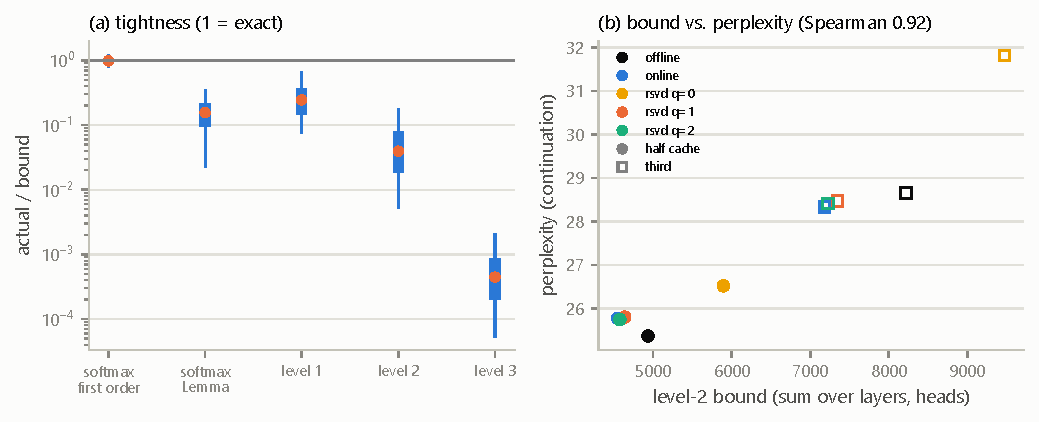
\includegraphics[width=0.72\textwidth]{figures/fig15_kv_bound.pdf}
\caption{The first bound on GPT-2. (a) Tightness: actual value divided by its bound (1 = exact; dot: median, bar: middle half, line: 5--95\%). ``First order'' is the attention-weighted term of Lemma~\ref{lem:softmax}, which is an estimate, not a bound. Levels 1--3 are the two inequalities of Proposition~\ref{prop:attnout} and Corollary~\ref{cor:resid}. (b) Level-2 bound, summed over layers and heads, against perplexity, for the five bases at half (filled) and a third (open) of the cache.}
\label{fig:kvbound}
\end{figure}

\paragraph{Check on GPT-2} (Figure~\ref{fig:kvbound}; numbers in Table~\ref{tab:boundsummary}).
\begin{itemize}[leftmargin=2em,itemsep=1pt]
\item \emph{\rl{B1} (every inequality holds) passes}: no violation in about 5.9 million cases.
\item \emph{\rl{B2} (level~2 within $10\times$ of the actual error) fails: level~2 is about $25\times$ too large.} The loss comes from the spread $\osc(\delta)$, which is set by the worst pair of scores while the attention sits on a few tokens. The lemma alone is $6\times$ too large, but its first-order term matches the actual change $\lVert\hat a-a\rVert_1$ almost exactly. Level~3 (Corollary~\ref{cor:resid}) is about $2250\times$ too large: the worst row of the prompt residual is only about $5\%$ of its Frobenius norm, and the Cauchy--Schwarz step loses the rest.
\item \emph{\rl{B3} (ranking with Spearman $\ge0.8$) passes, roughly.} Level~2 reaches $0.92$, the actual one-layer output error $0.99$. The 10 settings form two clusters (half and a third of the cache), so these values are rough. The whole gap between $0.92$ and $0.99$ is the offline basis being ranked 4th instead of 1st among the five half-cache bases: three misordered pairs (offline against online, RSVD $q=2$ and RSVD $q=1$). Perplexity puts the offline basis ahead of the online one ($25.37$ vs.\ $25.78$). A planned comparison with five trivial proxies (mean weighted residual of all or of the new tokens, its square, the attention-weighted value error, the attention-weighted score error) gives exactly $0.92$ for every one. So levels~2 and~2$'$ (Section~\ref{sec:bound2}) add no ranking information beyond such proxies; only level~V (Section~\ref{sec:bound3}) reaches the $0.99$ of the actual error.
\end{itemize}

\paragraph{Why the online basis loses to the offline one (\rl{R2}).}
Theorem~\ref{thm:exp} guarantees a small residual only on the prompt rows the basis was computed from. On the tokens after the prompt, the residuals of the exact online basis are $2.4\times$ (keys) and $6.2\times$ (values) larger than on the prompt (root mean square, half cache, median over layers and windows); for the offline basis the ratio is $1.00$ for both. The online basis fits its own prompt too closely, especially for values, where $512$ directions are fitted to $767$ rows. RSVD without power iterations has a smaller gap ($1.7\times$ and $2.8\times$) but a larger residual on the prompt, so in the end it is worse.

\means The proved bound holds everywhere and its constants cannot be lowered in general, but on real attention it is about $25\times$ too pessimistic. The useful quantity is its first-order form: score errors weighted by the attention each token receives. The check also showed why the online basis falls behind, a gap the theorem cannot see; Section~\ref{sec:kvupdate} attacks it.

\subsection{A tighter bound, weighted by attention}
\label{sec:bound2}

The first bound looks only at the worst pair of score errors and the worst value, yet its first-order term was nearly exact. We now make that term rigorous. Let $\bar\delta=\sum_ja_j\delta_j$ be the attention-weighted mean score error and $d_i=\delta_i-\bar\delta$ the error of token $i$ relative to it (a common shift changes nothing, as before). Write $\varphi(x)=e^x-1-x\ge0$, which is about $x^2/2$ for small $x$, and
\[
m_1=\sum_ia_i\lvert d_i\rvert,\qquad r=\sum_ia_i\varphi(d_i),\qquad \sigma_-^2=\sum_{i:\,d_i<0}a_id_i^2 .
\]
Here $m_1$ is the first-order term of Lemma~\ref{lem:softmax}, and $r\ge0$ is of second order (small when the errors are small).

\begin{lemma}[Attention-weighted softmax bound]\label{lem:softmax2}
The new weights are $\hat a_i=a_ie^{d_i}/(1+r)$, and
\[
\frac{m_1-\tfrac12\sigma_-^2-r}{1+r}\;\le\;\lVert\hat a-a\rVert_1\;\le\;\frac{m_1+2r}{1+r}.
\]
\end{lemma}

\plain The change in the attention weights equals the attention-weighted average score error $m_1$, up to second-order terms on both sides. So, \emph{to first order}, an error on a token that gets almost no attention costs almost nothing. The approximation $\lVert\hat a-a\rVert_1\approx m_1$ is good only when all $\lvert d_i\rvert$ are small. Large positive errors can make the change large: a token's weight is multiplied by $e^{d_i}$, which shows up in $r$. With two tokens, $a=(1-10^{-6},10^{-6})$ and $\delta=(0,20)$, the second token takes almost all the attention, and $\lVert\hat a-a\rVert_1$ is close to its largest possible value, 2. Large negative errors make $m_1$ an overestimate: with $a=(10^{-6},1-10^{-6})$ and $\delta=(-20,0)$ the actual change is $2.0\times10^{-6}$, while $m_1=4.0\times10^{-5}$ and the upper side is $7.8\times10^{-5}$.

\begin{proposition}[Attention-weighted output bound]\label{prop:attnout2}
With $u_i=\lVert(v_i-o)W\rVert$ (how far token $i$'s value is from the exact output) and $\varepsilon_i=\lVert(\hat v_i-v_i)W\rVert$ (its value error),
\[
\lVert(\hat o-o)W\rVert\;\le\;\underbrace{\sum_i\lvert\hat a_i-a_i\rvert\,u_i+\sum_i\hat a_i\varepsilon_i}_{\text{level }1'}
\;\le\;\underbrace{\frac{1}{1+r}\sum_ia_i\Bigl[\bigl(\lvert d_i\rvert+\varphi(d_i)+r\bigr)u_i+e^{d_i}\varepsilon_i\Bigr]}_{\text{level }2'}.
\]
To first order the right side is $\sum_ia_i\bigl(\lvert d_i\rvert u_i+\varepsilon_i\bigr)$.
\end{proposition}

\plain To first order, each token contributes in proportion to the attention it receives: its score error times how far its value is from the output, plus its value error (a large positive score error can still matter through $e^{d_i}$). Like level~2, level~2$'$ needs only the exact attention and the stored errors. So the residuals that matter are mainly those of tokens that receive attention. A basis that weights each token's row by its attention would target this directly; storing the first token exactly is the extreme case. Section~\ref{sec:kvattn} tests that idea.

\begin{figure}[!tb]
\centering
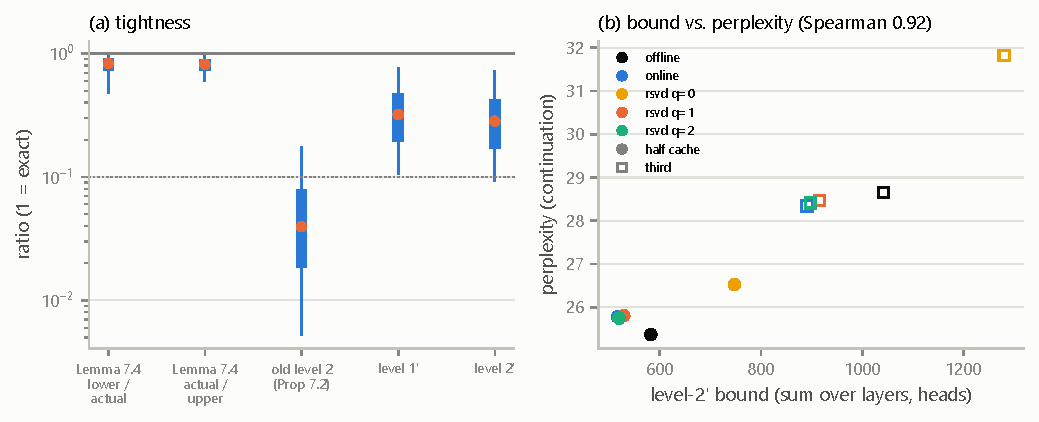
\includegraphics[width=0.9\textwidth]{figures/fig17_kv_bound2_fr.pdf}
\caption{The attention-weighted bound on GPT-2 (same setting as Figure~\ref{fig:kvbound}). (a) Tightness: lower side of Lemma~\ref{lem:softmax2} over the actual change, actual change over the upper side, and actual output error over the old level~2 and the new levels~1$'$ and~2$'$ (1 = exact; dotted: the $10\times$ target). (b) Level-2$'$ bound, summed over layers and heads, against perplexity. }
\label{fig:kvbound2}
\end{figure}

\paragraph{Check on GPT-2} (Figure~\ref{fig:kvbound2}; numbers in Table~\ref{tab:boundsummary}). First, a random stress test (\texttt{bound2\_random\_test.py}) found no violation in 20{,}000 random cases, and both sides of Lemma~\ref{lem:softmax2} are attained to within $10^{-6}$. On GPT-2:
\begin{itemize}[leftmargin=2em,itemsep=1pt]
\item \emph{\rl{T1} (both lemmas and levels~1$'$, 2$'$ hold in every case) fails as written, but only through rounding.} Levels~1$'$ and~2$'$ and the lower side of the lemma always hold. The upper side was exceeded by at most $1.5\times10^{-7}$ (relative), more than the $10^{-9}$ we allowed. We recomputed the worst case with 50-digit arithmetic (\texttt{bound2\_hp\_check.py}). There the change in the weights is only $2.1\times10^{-9}$, the bound holds (ratio $0.9999999986$), and the float64 value was off by $3\times10^{-16}$. Our tolerance was too small for such tiny changes.
\item \emph{\rl{T2} (level~2$'$ within $10\times$) passes}: level~2$'$ is a median $3.5\times$ the actual error, $7\times$ tighter than level~2.
\item \emph{\rl{T3} (upper side of Lemma~\ref{lem:softmax2} within 25\% of $\lVert\hat a-a\rVert_1$, median ratio $\ge0.8$) passes narrowly}: the upper side is a median $1.2\times$ the actual change, the lower side $0.83\times$. At a third of the cache, where the score errors are larger, the upper side is less tight ($0.73$--$0.78$ by method, against $0.83$--$0.87$ at half).
\item \emph{\rl{T4} (ranking) passes} with Spearman $0.92$, the same value as level~2 and with the same misranking of the offline basis.
\end{itemize}
Levels~1$'$ and~2$'$ are nearly equal. We expected the remaining factor of about $3.5$ to come from a step they share: adding the error vectors of different tokens by their lengths (the triangle inequality $\lVert x+y\rVert\le\lVert x\rVert+\lVert y\rVert$), when in reality they partly cancel. Section~\ref{sec:bound3} tests this and finds that it explains only part of the looseness.

\subsection{A variance form of the bound}
\label{sec:bound3}

Both sums in Proposition~\ref{prop:attnout2} can instead be bounded as a whole, by the Cauchy--Schwarz inequality in matrix form. Write $y_i=(v_i-o)W$ and $\vec\varepsilon_i=(\hat v_i-v_i)W$ for the row vectors whose lengths are $u_i$ and $\varepsilon_i$, and
\[
C_y=\sum_ia_i\,y_i\T y_i,\qquad C_\varepsilon=\sum_i\hat a_i\,\vec\varepsilon_i\T\vec\varepsilon_i,\qquad \chi^2=\sum_i\frac{(\hat a_i-a_i)^2}{a_i}.
\]
$C_y$ is the spread of the values around the output, weighted by attention; its largest eigenvalue $\lambda_{\max}(C_y)$ is the largest attention-weighted variance of the values in any single direction. $C_\varepsilon$ is the same for the value errors. $\chi^2$ is the \emph{chi-squared distance} between the new and the old attention weights, a standard measure of how different two probability distributions are.

\begin{proposition}[Variance form of the output bound]\label{prop:attnout3}
\[
\lVert(\hat o-o)W\rVert\;\le\;\sqrt{\lambda_{\max}(C_y)\,\chi^2}\;+\;\sqrt{\lambda_{\max}(C_\varepsilon)},
\qquad
\chi^2=\frac{\sum_ia_ie^{2d_i}}{(1+r)^2}-1.
\]
To first order $\chi^2=\sum_ia_id_i^2$, the attention-weighted variance of the score errors. Each term on its own can be attained with equality (see the proof).
\end{proposition}

\plain The mixing term is (spread of the score errors) times (spread of the values), both measured as attention-weighted standard deviations, and the values only in their widest direction. The value term is the largest attention-weighted root-mean-square value error in any one direction. Proposition~\ref{prop:attnout2} adds lengths; this bound uses only the widest direction. It gains when the spread is shared among many directions ($\lambda_{\max}$ much smaller than the total spread $\tr C_y$) and can also be larger. Since both bounds hold, the smaller of the two can be taken for each term (``level~C''). The inequality is a standard Cauchy--Schwarz (chi-squared change-of-measure) argument; what we add is its test on real attention.

\begin{figure}[!tb]
\centering
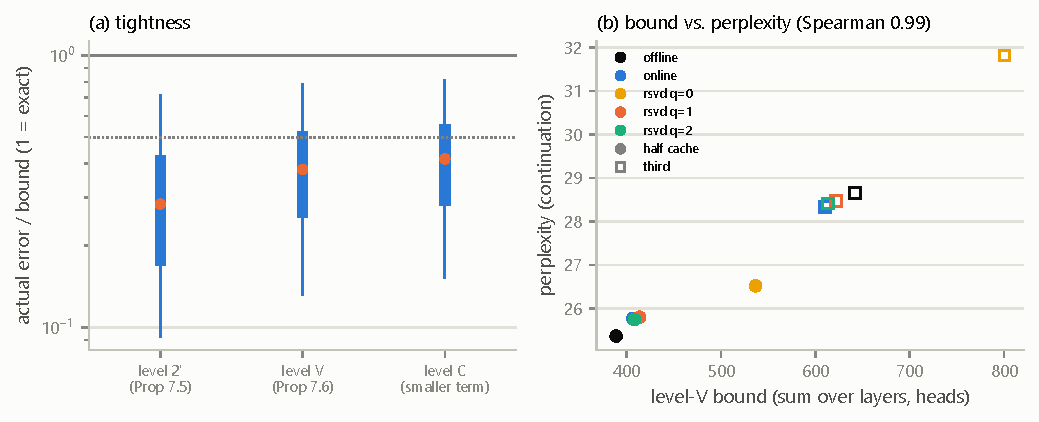
\includegraphics[width=0.9\textwidth]{figures/fig21_kv_bound3_fr.pdf}
\caption{The variance-form bound on GPT-2, every fourth continuation query. (a) Tightness for level~2$'$, level~V (Proposition~\ref{prop:attnout3}) and level~C (the smaller of the two for each term) (1 = exact; dot: median, bar: middle half, line: 5--95\%; dotted: the $2\times$ target of \rl{V3}). (b) Level-V bound, summed over layers and heads, against perplexity, for the five bases at half (filled) and a third (open) of the cache. }
\label{fig:kvbound3}
\end{figure}

\paragraph{Check} (Figure~\ref{fig:kvbound3}; numbers in Table~\ref{tab:boundsummary}). In 20{,}000 random cases (\texttt{bound3\_random\_test.py}) the bound held, with a worst ratio of exactly $1$ up to rounding, and the two equality cases give ratio $1$. On GPT-2 we used every fourth continuation query (about 1.5 million cases; violations are checked on all of them, medians and percentiles on every third case).
\begin{itemize}[leftmargin=2em,itemsep=1pt]
\item \emph{\rl{V1} (level~V holds in every case) and \rl{V4} (ranking) pass.} There is no violation. Level~V ranks the settings with Spearman $0.99$, the same as the actual one-layer error, and puts the offline basis ahead of the online one at half the cache ($389$ vs.\ $407$), as perplexity does. It orders the five half-cache bases exactly as the actual one-layer error does; both differ from perplexity by one adjacent swap (online $25.775$ vs.\ RSVD $q=2$ $25.747$).
\item \emph{\rl{V2} (at least $1.5\times$ tighter than level~2$'$) and \rl{V3} (level~C within $2\times$ of the actual error) fail.} Level~V is a median $2.6\times$ the actual error (5--95\%: $1.3$ to $7.6\times$ too large), against $3.5\times$ for level~2$'$, so it is only $1.31\times$ tighter (median; 5--95\%: $0.74$--$2.29$). Level~C is $2.4\times$ the actual error. The variance form is the smaller one for the mixing term in $93\%$ of cases and for the value term in $65\%$.
\item \emph{Why the gain is small.} A rough guide (not a theorem): when the spread is shared evenly among $n$ directions, $\lambda_{\max}=\tr C/n$, so the variance form is smaller by about $\sqrt n$. On real attention that number is small: the \emph{effective rank} (trace divided by largest eigenvalue, roughly the number of directions that carry the spread) of $C_y$ and $C_\varepsilon$ is a median $2.9$ and $2.7$. Attention sits on a few tokens, so the errors that matter point in only two or three directions.
\end{itemize}
So the triangle inequality explains only part of the looseness. The remaining factor of about $2.5$ is the Cauchy--Schwarz step itself: the actual error vector is not lined up with the widest direction of the values, and the score errors are not proportional to the values' deviations.

\begin{table}[!tb]
\centering\footnotesize
\setlength{\tabcolsep}{4pt}
\begin{tabular*}{\textwidth}{@{\extracolsep{\fill}}llrcrc@{}}
\toprule
bound & needs & tightness & 5--95\% & Spearman & offline/online\\
\midrule
\multicolumn{6}{@{}l}{\emph{Attention weights only} (ratio to $\lVert\hat a-a\rVert_1$)}\\
Lemma~\ref{lem:softmax} ($\tfrac12\osc(\delta)$) & score errors & $0.16$ & -- & -- & --\\
first-order term $m_1$ (estimate) & score errors & $0.98$ & $0.81$--$1.20$ & -- & --\\
Lemma~\ref{lem:softmax2}, upper side & score errors & $0.82$ & $0.60$--$0.96$ & -- & --\\
Lemma~\ref{lem:softmax2}, lower side & score errors & $0.83$ & -- & -- & --\\
\midrule
\multicolumn{6}{@{}l}{\emph{Attention output} (ratio to $\lVert(\hat o-o)W_O^h\rVert$)}\\
level 3 (Cor.~\ref{cor:resid}) & largest residual rows & $0.00044$ & -- & -- & --\\
level 2 (Prop.~\ref{prop:attnout}) & stored errors & $0.039$ & $0.005$--$0.17$ & $0.92$ & wrong\\
level 1 (Prop.~\ref{prop:attnout}) & actual weights & $0.24$ & -- & -- & --\\
level 2$'$ (Prop.~\ref{prop:attnout2}) & stored errors & $0.28$ & $0.09$--$0.71$ & $0.92$ & wrong\\
level 1$'$ (Prop.~\ref{prop:attnout2}) & actual weights & $0.32$ & -- & -- & --\\
level V (Prop.~\ref{prop:attnout3}) & stored errors & $0.38$ & $0.13$--$0.78$ & $0.99$ & right\\
level C (smaller of 2$'$ and V) & stored errors & $0.42$ & -- & -- & --\\
trivial residual proxies (5) & stored errors & -- & -- & $0.92$ & 2 of 5 right\\
\midrule
actual one-layer error & -- & $1$ & -- & $0.99$ & right\\
\bottomrule
\end{tabular*}
\caption{Summary of the attention-output bounds on GPT-2 (Sections~\ref{sec:bound1}--\ref{sec:bound3}). ``Tightness'': median of the actual quantity divided by the bound (1 = exact; $0.1$ = $10\times$ too large); for the lower side of Lemma~\ref{lem:softmax2} it is the bound divided by the actual change, and for the first-order term the actual change divided by the estimate. ``5--95\%'': spread of that ratio over all cases. ``Needs'': ``score errors'' and ``stored errors'' mean only the exact attention and the errors of the stored keys (and values) are needed; ``actual weights'' means $\lVert\hat a-a\rVert_1$ itself is needed. ``Spearman'': rank correlation of the bound (summed over layers and heads) with perplexity over the 10 settings. ``Offline/online'': whether the bound orders these two bases at half the cache as perplexity does; levels 2 and 2$'$ rank the offline basis 4th instead of 1st among the five half-cache bases, the whole gap between $0.92$ and $0.99$. The five trivial proxies all give the same ranking (Spearman $0.92$); the offline-4th explanation is stated only for levels 2 and 2$'$. No bound was violated, apart from float64 rounding at the $10^{-7}$ level (Section~\ref{sec:bound2}). Dashes: not computed.}
\label{tab:boundsummary}
\end{table}

\means Each step from the first bound to the variance form replaced a worst case by an attention-weighted average and gained tightness: from $25\times$ to $3.5\times$ to $2.6\times$ the actual error ($2.4\times$ for level~C). The softmax part is now accurate to about 20\% from both sides. The bounds agree with two practical findings: the attention-sink token must be kept accurately because errors count (to first order) by attention, and the online basis loses because new tokens fit it worse than the prompt. Only the variance form ranks the bases better than trivial residual proxies. Each bound covers one attention operation, not how errors pass from layer to layer: compressing all 12 layers costs $1.57$ times the sum of the single-layer excess losses (Section~\ref{sec:kvadditive}), so one-layer errors and bounds should not be summed. Splitting the output error into a part from changed attention weights and a value part is natural, and recent methods also control the attention-output error \cite{readkv2026,anchorkv2026}; we did not find measurements of how tight such bounds are on real attention, or why (attention concentrates on two or three directions), in the parts of those papers that we read.

% =====================================================================

% ---- end short/s06_07_prompt_bounds ----
% ---- begin short/s08a_update_core ----
\section{Updating the basis during generation}
\label{sec:kvupdate}
% =====================================================================

The online basis of Section~\ref{sec:kvonline} is computed once, from the prompt. Later tokens fit it $2.4\times$ (keys) and $6.2\times$ (values) worse than the prompt itself (Section~\ref{sec:bound1}), which is why it loses to the offline basis. Here the basis keeps learning from the new tokens. The design is close to iS-KV \cite{iskv2026}, found only after these experiments (Section~\ref{sec:relwork}). Planned tests then ask which ingredient does the work (Section~\ref{sec:kvbuffer}), whether attention weighting helps (Section~\ref{sec:kvattn}) and how to make the update cheaper (Section~\ref{sec:kvcheap}). Section~\ref{sec:kvchecks} compares the recipe with quantization and eviction at equal memory, probes copying and generation, and repeats it on a model with rotary positions. Sections~\ref{sec:kvround3} and~\ref{sec:kvadditive} hold later planned follow-ups: why the two models differ, quantized codes and recency controls; then sinks, heads, a change of domain and additivity over layers. Follow-up experiments are numbered C1--C23 after their result files (Section~\ref{sec:measure}); earlier sections give only the conclusions of C14--C23.

\subsection{The block scheme and its results}
\label{sec:blockscheme}

Everything is as in Section~\ref{sec:kvonline} (one basis per layer, query-aware keys, output-aware values, mean removed, first token exact, 16 windows, perplexity on the continuation only), except that the continuation is processed in \emph{blocks} of $B$ tokens. While a block is processed, its own keys and values are kept exact: a \emph{recent buffer} of at most $B$ tokens. At the end of the block, every layer does three steps.
\begin{enumerate}[leftmargin=2em,itemsep=0pt]
\item \emph{Update.} The summary of everything seen so far is the current basis $U$ ($768\times R$) with its singular values $S$. The block's exact weighted rows $A_{\mathrm{blk}}=(X_{\mathrm{blk}}-\mu)G^{1/2}$ are stacked under it, and the new basis $U'$ is given by the top $R$ right singular vectors of $\begin{bsmallmatrix}SU\T\\ A_{\mathrm{blk}}\end{bsmallmatrix}$ ($R+B$ rows). This is the standard \emph{incremental SVD}: without truncation it would equal an SVD of all rows seen so far.
\item \emph{Re-projection.} Old stored codes $c$ (one row of $R$ numbers per token) move into the new basis, $c\mapsto cU\T U'$; the part of an old entry outside the new basis is lost.
\item \emph{Compression.} The block itself is stored in the new basis.
\end{enumerate}
The mean $\mu$ and the weights $G$ stay as computed from the prompt. All methods, including those that never update, use the same block scheme. Running the continuation block by block with the full cache reproduces a single pass (largest logit difference $0.0021$).
We compare the \emph{static} prompt basis and the \emph{offline} calibration basis (both never updated) with the \emph{update} and four variants: \emph{decay} (the summary is scaled by $0.9$ before each block, so recent text counts more), \emph{no re-projection} (old entries keep their basis; impractical, but it shows what re-projection costs), \emph{RSVD + update} (an RSVD prompt basis with one power iteration as the start) and an \emph{oracle} that refits an exact SVD on all exact rows at every block and compresses the whole cache again (not realizable, since it needs the exact old cache; it shows the best an update of this size can do). Rules \rl{U1}--\rl{U4} are in Table~\ref{tab:rules}.

\begin{figure}[!tb]
\centering
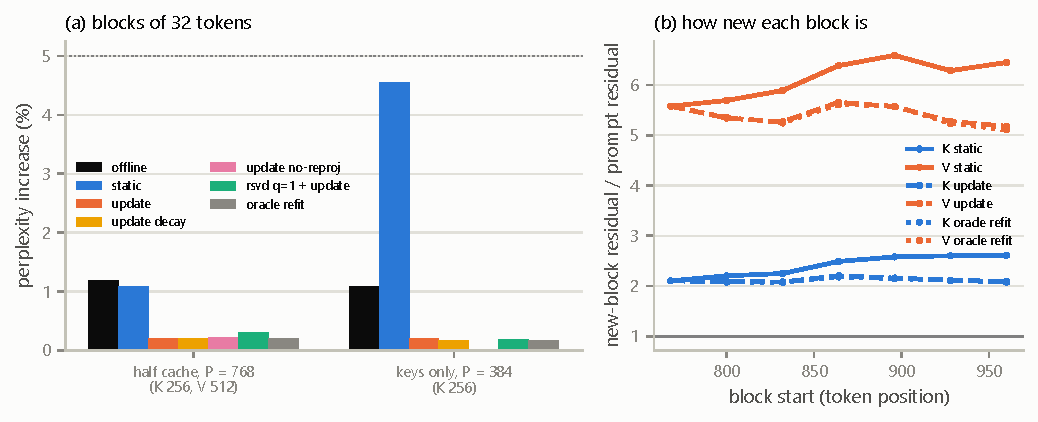
\includegraphics[width=0.9\textwidth]{figures/fig16_kv_update.pdf}
\caption{Basis updated during generation. (a) Perplexity increase over the full cache, blocks of 32 tokens; dotted line: $+5\%$. (b) How new each block is: the residual of a block's weighted rows outside the current basis (before the update), divided by the residual of the prompt rows under the prompt basis; median over layers and windows, half cache, $P=768$, against the block's position in the continuation. A value of 1 means the block fits as well as the prompt did.}
\label{fig:kvupdate}
\end{figure}

\paragraph{Results} (Figure~\ref{fig:kvupdate}; 4080 continuation tokens at $P=768$, 10{,}224 at $P=384$).
\emph{All four rules pass.} After a 768-token prompt, with keys at $R=256$ and values at $R=512$ (half the stored codes) and $B=32$, the full cache gives $24.73$, the offline basis $25.02$ ($+1.2\%$), the static basis $25.00$ ($+1.1\%$) and the updated basis $24.78$ ($+0.20\%$, \rl{U1}). The RSVD start gives $24.80$, $0.1\%$ above the exact start (\rl{U2}) and $+0.3\%$ over the full cache (\rl{U3}). With a 384-token prompt and keys only (full cache $26.70$): offline $+1.1\%$, static $+4.5\%$, update $+0.2\%$, so the update removes $96\%$ of the static loss (\rl{U4}). Counting the per-prompt basis and the buffer (Proposition~\ref{prop:kvmem}), the static and updated caches need $0.92$ of the full cache at 1024 tokens ($0.83$ keys only); the offline basis with the buffer needs $0.52$ ($0.68$).
\begin{itemize}[leftmargin=2em,itemsep=1pt]
\item \emph{Post hoc: most of the gain over Section~\ref{sec:kvonline} comes from the buffer, not from the update.} With every token compressed at once, the static basis cost $+4.2\%$ and the offline one $+2.6\%$. Keeping only the current block exact (on average 16 recent tokens, at most 32) lowers these to $+1.1\%$ and $+1.2\%$. A likely reason: recent tokens tend to receive much of the attention, and by Lemma~\ref{lem:softmax2} errors count in proportion to attention. The update then removes about $80\%$ of what remains. With the short prompt the update matters more ($+9.8\%\to+4.5\%\to+0.2\%$). The buffer is cheap: 32 exact tokens cost at most 16 extra full-token entries, $1.6\%$ of the full cache at 1024 tokens ($3.1\%$ of the half-size cache).
\item \emph{The simple update is close to the best this scheme can do.} It is indistinguishable at our resolution from the oracle ($24.778$ vs.\ $24.775$; $26.755$ vs.\ $26.745$ at $P=384$). Without re-projection it gives $24.782$, with decay $24.776$: differences of $0.04\%$ or less. On fresh windows 16--31 with paired bootstrap intervals (Table~\ref{tab:fu-buffer}), decay shows a borderline gain of $0.065\%$ (its interval just excludes 1; one of six intervals, no correction for multiple comparisons); re-projection, the oracle and the RSVD start stay indistinguishable from the plain update. Blocks of 128 tokens (memory $0.97$) give the same $+0.2\%$, but there the larger buffer alone already brings the static basis to $+0.5\%$.
\item \emph{New tokens fit worse than old ones} (Figure~\ref{fig:kvupdate}(b)). Under the static basis the per-block ratio grows from about $2.1$ to $2.6$ (keys) and $5.6$ to $6.5$ (values); with the update it stays near $2.1$ and $5.2$--$5.7$, as for the oracle. So the $2.4\times$/$6.2\times$ gap is mostly not a stale basis. It is consistent, at least in part, with the out-of-sample error of a basis fitted to few rows ($R/n\approx0.33$ for keys, $0.67$ for values). A basis fitted to the first half of the prompt fits the held-out second half $3.21\times$ (keys) and $5.60\times$ (values) worse than its own rows, against $4.27\times$ and $5.88\times$ for the continuation (rule \rl{N1} passes, for keys only just: $0.752$ against $0.75$). An interleaved split (Section~\ref{sec:kvround3}) shows that the gap is out-of-sample error \emph{plus} drift of the text, drift mattering most for keys. A Gaussian model with the same covariance predicts only $1.63$ and $3.38$ against the measured $2.47$ and $6.19$ (rule \rl{N2} fails; about $45\%$ of the excess gap). No update can remove this error, since each block is new when it arrives; the update stops the gap from \emph{growing}.
\item \emph{Cost.} One update is an SVD of an $(R+B)\times768$ matrix per layer: $36$\,ms (keys) and $99$\,ms (values) with $B=32$ (median, CPU; another session measured $53$ and $151$\,ms, Section~\ref{sec:kvcheap}, so compare only within a run). That is about $1.6$\,s per block for 12 layers, or about $50$\,ms per token in steady state (one update's time divided by the tokens between updates), close to generating a token ($36$--$47$\,ms with a short cache, Section~\ref{sec:quality} and Appendix~\ref{app:rerun}; $64$\,ms with about 1000 cached tokens). Every 128 tokens it is $58$ and $131$\,ms, about $18$\,ms per token. Re-projection costs about $TR^2$ multiply-adds per layer for $T$ cached tokens, as much as $R/12\approx21$ (keys) and $43$ (values) decode steps of factored attention (counted, not timed).
\end{itemize}

\means With a small exact buffer and a basis updated every 32--128 tokens, half the stored codes, computed from the text itself, cost only $0.2\%$ in perplexity, better than the offline basis. Two cautions: the per-prompt basis makes this cache $0.92$ of the full memory at GPT-2's 1024 tokens (offline with the buffer: $+1.2\%$ at $0.52$), and 768 of the 1024 cached tokens are the prompt the basis was fitted to. Planned follow-ups address the second: on fresh windows 16--31 the result is $+0.21\%$ (rule \rl{Q1} passes); after a 256-token prompt, so that 768 cached tokens are new, the update gives $+0.20\%$, against $+1.17\%$ for the offline basis and $+0.45\%$ for the offline basis with the update (rules \rl{P1}, \rl{P2} pass). The static basis costs $+27.6\%$ there, but 255 prompt rows cap it at rank 254, so that is not a fair baseline. An offline basis updated in the same way reaches only $+0.87\%$ against $+0.20\%$ (item \rl{N3}): the update does not rescue a basis computed from other text.

\subsection{Buffer or update? A planned test}
\label{sec:kvbuffer}

The buffer comparison above was post hoc, so a planned $2\times2$ test switches the two ingredients. \emph{Buffer off}: each new key and value is compressed before attention reads it, including the token's own attention, which no real cache would do. \emph{Update off}: the static prompt basis. ``Buffer off'' still keeps the block's exact rows for the update, so it saves no memory. Three of the four cells had been measured before and were reproduced exactly; only ``update only'' and a sweep of buffer sizes for the static basis were new. Rules \rl{F1}--\rl{F4} are in Table~\ref{tab:rules}.

\begin{figure}[!tb]
\centering
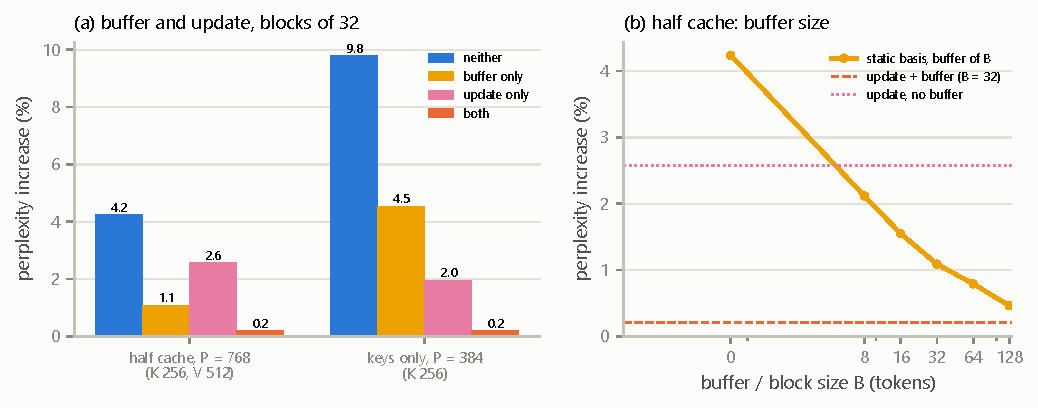
\includegraphics[width=0.85\textwidth]{figures/fig18_kv_buffer.pdf}
\caption{Buffer or update: perplexity increase over the full cache on the continuation tokens, 16 test windows, updates every 32 tokens. (a) The four combinations, half the codes after a 768-token prompt (memory $0.91$ for ``neither'', $0.92$ for the others, including the per-prompt basis) and keys only after a 384-token prompt ($0.82$ and $0.83$). ``Update only'' keeps the block's exact rows for the update, so it needs the same memory as ``both''. (b) Half cache: the static basis against the buffer size $B$ ($B=0$: no buffer); horizontal lines: the update without buffer, and with a 32-token buffer.}
\label{fig:kvbuffer}
\end{figure}

\paragraph{Results} (Figure~\ref{fig:kvbuffer}).
\begin{itemize}[leftmargin=2em,itemsep=1pt]
\item \emph{\rl{F1} fails; \rl{F2}, \rl{F3} and \rl{F4} pass.} With half the codes (full cache $24.73$), ``neither'' gives $25.78$ ($+4.24\%$), the buffer only $25.00$ ($+1.09\%$), the update only $25.37$ ($+2.58\%$) and both $24.78$ ($+0.20\%$). The buffer alone removes $74\%$ of the excess; the update alone only $39\%$ (half was asked), no better than the offline basis ($25.365$ and $25.368$, equal by coincidence). Keys only after a 384-token prompt: $+9.8\%$, $+4.5\%$, $+2.0\%$, $+0.2\%$; there the update alone does more than the buffer alone, and \rl{F1}--\rl{F3} all hold.
\item \emph{The two help each other.} If each removed a fixed share of the excess independently, the leftover shares would multiply: $4.2\%\times\frac{1.1}{4.2}\times\frac{2.6}{4.2}\approx0.7\%$. The actual $0.2\%$ is about a third of that ($0.9\%$ expected, $0.2\%$ measured with the short prompt). A plausible reading: the update keeps the basis fitting older text, while the buffer protects the newest tokens, which the basis has not seen and which often receive much of the attention.
\item \emph{A larger buffer always helps the static basis} (\rl{F4}): $+4.2\%$, $+2.1\%$, $+1.6\%$, $+1.1\%$, $+0.8\%$, $+0.5\%$ for $B=0,8,16,32,64,128$; each doubling cuts the excess by $27$--$42\%$. On these windows $B=128$ ($+0.46\%$, memory $0.97$) is still worse than update + 32-token buffer ($+0.20\%$, $0.92$). On fresh windows 16--31, however, $B=128$ alone gives $+0.07\%$ and $B=64$ $+0.37\%$, against $+0.21\%$, and $B=128$ is indistinguishable from update + buffer (ratio $0.9987$, CI $0.9962$--$1.0008$; Table~\ref{tab:fu-buffer}). A larger buffer is thus a serious alternative: no update time, for about $5\%$ more memory at 1024 tokens.
\item \emph{Fresh windows (planned).} On windows 16--31 the four cells give $+3.45\%$, $+0.84\%$, $+2.42\%$ and $+0.21\%$, in the order asked by rule \rl{Q2} (passes); ``both'' is below ``buffer only'' with an interval below 1 (\rl{Q3} passes).
\item \emph{Which exact tokens matter (planned).} Keeping only a token's own entry exact removes just $18\%$ of the no-buffer excess ($+4.24\%\to+3.47\%$; \rl{S1} asked for $30\%$ and fails); the block buffer removes $69\%$ of what remains. Adding 31 random prompt tokens gives the same $+3.47\%$, the 31 most-attended prompt tokens $+3.46\%$ (the first token is exact in all variants). A sliding window of the 31 newest tokens gives $+0.77\%$ (\rl{S2} and \rl{S4} pass), but it holds about 31 exact tokens against about 16 for the block buffer; at equal average budget the two are not resolved (Section~\ref{sec:kvround3}), so we do not claim that a sliding window is better. Without a buffer, $80\%$ (keys) and $94\%$ (values) of the error that attention reads under the updated basis falls on tokens younger than 32 (\rl{S3} passes); with the block buffer, $26\%$ and $25\%$.
\item \emph{Recency or novelty? (planned).} The newest tokens are also those new to the basis. A control keeps 31 \emph{old continuation} tokens exact besides the own token (new to the basis, but not recent): ages 32--62 give $+3.13\%$, 31 random ones older than 32 $+3.37\%$, against $+3.47\%$ for the own token alone and $+0.77\%$ for the sliding window. Rules \rl{Z1} and \rl{Z2} (excess at most $2.12\%$) both fail: the gain needs the \emph{newest} tokens, recency rather than novelty alone. Caveats: one basis, one model, 16 windows; no extra exact token exists in the first 32 continuation steps and fewer than 31 until step 62 ($24\%$ of the steps), so the gap to the sliding window is an upper bound on what recency adds; and the exact rows come from an exact copy, a control rather than a realistic cache. Scored from step 63 on, without the ramp, the conclusion holds (Section~\ref{sec:kvround3}). A consistent but untested mechanism: in the full model, tokens of age 0--15 receive $27\%$ of the attention (the first token $37\%$).
\end{itemize}

\means The buffer is the larger single gain for the half-size cache, the update the larger one after a short prompt; together they beat both, also on fresh windows. The buffer works through exact storage of the \emph{newest} tokens, not of highly attended or older ones (with the caveats above). iS-KV uses both ingredients but does not separate them (OjaKV also keeps recent tokens at full rank, chosen by a score); this separation is one of our candidate contributions.

\begin{table}[!htb]
\centering\footnotesize
\begin{tabularx}{\textwidth}{@{}>{\raggedright}X >{\raggedleft}p{3.6cm} >{\raggedleft\arraybackslash}p{2.9cm}@{}}
\toprule
method (half the codes, $P=768$) & windows 16--31 & windows 0--15\\
\midrule
full cache (perplexity) & 24.93 & 24.73\\
static, no buffer & $+3.45\%$ & $+4.24\%$\\
static, own token exact ($B=1$) & -- & $+3.47\%$\\
static, own + 31 random prompt tokens & -- & $+3.47\%$\\
static, own + 31 most-attended prompt tokens & -- & $+3.46\%$\\
static, block buffer 8 / 16 / 32 / 64 / 128 & $+1.73$ / $1.37$ / $0.84$ / $0.37$ / $0.07\%$ & $+2.12$ / $1.55$ / $1.09$ / $0.79$ / $0.46\%$\\
static, own + 31 continuation tokens of age 32--62 & -- & $+3.13\%$\\
static, own + 31 random continuation tokens older than 32 & -- & $+3.37\%$\\
static, sliding window 32 & -- & $+0.77\%$\\
update, no buffer & $+2.42\%$ & $+2.58\%$\\
update, block buffer 32 & $+0.21\%$ & $+0.20\%$\\
offline, no buffer / block buffer 32 & $+2.50\%$ / $+1.13\%$ & $+2.59\%$ / $+1.19\%$\\
offline + update, block buffer 32 & -- & $+0.87\%$\\
\midrule
\multicolumn{3}{@{}>{\raggedright\arraybackslash}p{\textwidth}@{}}{\emph{ratios of perplexity, windows 16--31, with 95\% CI}}\\
both / buffer only & \multicolumn{2}{>{\raggedleft\arraybackslash}p{6.7cm}}{$0.9937$ ($0.9892$--$0.9977$), 13 of 16 windows}\\
update with decay / update (borderline) & \multicolumn{2}{>{\raggedleft\arraybackslash}p{6.7cm}}{$0.99935$ ($0.99880$--$0.99993$), 12 of 16}\\
no re-projection / update & \multicolumn{2}{>{\raggedleft\arraybackslash}p{6.7cm}}{$0.99978$ ($0.9994$--$1.0001$)}\\
oracle refit / update & \multicolumn{2}{>{\raggedleft\arraybackslash}p{6.7cm}}{$0.99978$ ($0.9991$--$1.0004$)}\\
RSVD $q=1$ + update / update & \multicolumn{2}{>{\raggedleft\arraybackslash}p{6.7cm}}{$0.99991$ ($0.9989$--$1.0009$)}\\
attn-late / unweighted, no buffer; buffer & \multicolumn{2}{>{\raggedleft\arraybackslash}p{6.7cm}}{$0.9987$ ($0.9960$--$1.0013$); $0.9996$ ($0.9979$--$1.0009$)}\\
\midrule
\multicolumn{3}{@{}>{\raggedright\arraybackslash}p{\textwidth}@{}}{\emph{ratios of perplexity, windows 0--15, with 95\% CI (which exact tokens matter)}}\\
most-attended / random prompt tokens & \multicolumn{2}{>{\raggedleft\arraybackslash}p{6.7cm}}{$0.99984$ ($0.9993$--$1.0003$)}\\
sliding window / random prompt tokens & \multicolumn{2}{>{\raggedleft\arraybackslash}p{6.7cm}}{$0.974$ ($0.964$--$0.983$), 16 of 16 windows}\\
sliding window / block buffer & \multicolumn{2}{>{\raggedleft\arraybackslash}p{6.7cm}}{$0.9969$ ($0.9938$--$0.9998$), 11 of 16}\\
lagged old tokens / own token only & \multicolumn{2}{>{\raggedleft\arraybackslash}p{6.7cm}}{$0.9967$ ($0.9931$--$0.9996$)}\\
random old tokens / own token only & \multicolumn{2}{>{\raggedleft\arraybackslash}p{6.7cm}}{$0.9991$ ($0.9976$--$1.0006$)}\\
lagged / sliding; random old / sliding & \multicolumn{2}{>{\raggedleft\arraybackslash}p{6.7cm}}{$1.023$ ($1.012$--$1.036$); $1.026$ ($1.016$--$1.037$), 0 of 16}\\
\midrule
\multicolumn{3}{@{}>{\raggedright\arraybackslash}p{\textwidth}@{}}{\emph{prompt of 256 tokens (768 new tokens), windows 0--15, full cache 26.84}}\\
static (rank capped at 254) / update / offline / offline + update & \multicolumn{2}{>{\raggedleft\arraybackslash}p{6.7cm}}{$+27.64\%$ / $+0.20\%$ / $+1.17\%$ / $+0.45\%$}\\
\bottomrule
\end{tabularx}
\caption{Buffer and update follow-ups of Sections~\ref{sec:blockscheme} and~\ref{sec:kvbuffer} (\texttt{c1\_*.json}, \texttt{c2\_kv\_synergy.json}, \texttt{c3\_kv\_novelty.json}, \texttt{c4\_kv\_p256.json}, \texttt{c12\_kv\_control.json}). ``Own token exact'': only the token being processed is read exactly. ``Sliding window'': the 32 most recent tokens. The offline + update row is the planned check of Section~\ref{sec:blockscheme}.}
\label{tab:fu-buffer}
\end{table}

\subsection{A basis weighted by attention: a planned test}
\label{sec:kvattn}

Proposition~\ref{prop:attnout2} counts each token's error by the attention it receives, while the prompt basis counts every prompt token equally. So we scaled each prompt row of the SVD by $\sqrt{w_i}$, where $w_i$ is the attention token $i$ receives in the exact prefill, averaged over the 12 heads and divided by its mean. \emph{Attn-late} (the rule method) takes $w_i$ from the last 128 prompt queries, which, like future queries, see almost every prompt token; \emph{attn-all} uses all prompt queries, \emph{mix-late} is half uniform, half attn-late. To see where the error sits, we weight each token's residual $\rho_i=\lVert(x_i-\hat x_i)G^{1/2}\rVert^2$ by the head-averaged attention of the continuation queries in a full-cache pass, and split the sum into $D_{\mathrm{prompt}}$ (prompt tokens) and $D_{\mathrm{cont}}$ (continuation tokens).

\emph{Result} (16 windows; rules \rl{W1}--\rl{W3} fail, \rl{W4} passes; Table~\ref{tab:rules}): no weighting helps by more than $0.25$ points anywhere. At half cache with every token compressed, attn-late gives $+4.15\%$ against $+4.24\%$ unweighted, removing only $2\%$ of the excess (on fresh windows the ratio's interval is $0.9960$--$1.0013$, unresolved), and stays behind the offline basis ($+2.6\%$); with the 32-token buffer it is slightly worse ($+1.16\%$ against $+1.09\%$). Attn-late is clearly worse with a third of the cache (keys 128, values 384: $+17.3\%$ against $+14.6\%$; with the buffer $+7.5\%$ against $+5.6\%$) and with keys only after a 384-token prompt ($+11.3\%$ against $+9.8\%$; with the buffer $+5.3\%$ against $+4.5\%$).

The weighting does work on the prompt: $D_{\mathrm{prompt}}$ drops to $0.95\times$ (keys) and $0.87\times$ (values) (\rl{W4}). But with every token compressed, $93\%$ (keys) and $99\%$ (values) of $D_{\mathrm{prompt}}+D_{\mathrm{cont}}$ lies on the continuation's own tokens, which are new to the basis. There the weighted basis is slightly worse ($D_{\mathrm{cont}}$ $1.07\times$ and $1.06\times$), since it rests on fewer \emph{effective} rows: $(\sum w_i)^2/\sum w_i^2$ is only $29\%$ of the row count. The offline basis has $D_{\mathrm{cont}}$ of $0.76\times$ and $0.38\times$ the unweighted one, which is why it wins without a buffer.

\means Weighting the \emph{prompt} rows cannot reach the error that matters: it sits on tokens the basis has not seen, where the buffer and the update help. AttSVD \cite{attsvd2026} weights by attention but keeps new tokens exact; in that mode on GPT-2 the weighting still gives nothing (Section~\ref{sec:kvround3}), so this does not reconcile the two results (SnapKV \cite{li2024snapkv} uses prefill attention to \emph{evict} tokens instead). One blind spot of $D$: low-attention prompt tokens with positive score errors gain attention that $D$ does not count, but they carry only about $4\%$ of the change in the attention weights. The finding is specific to GPT-2: on a small model with rotary positions the weighted basis helps (Section~\ref{sec:kvchecks}). An attention-weighted \emph{update} is untested; the plain update is already indistinguishable from the oracle.

\subsection{A cheaper update: a planned test}
\label{sec:kvcheap}

The update costs about as much time as generation (Section~\ref{sec:blockscheme}). We tried two ways to make it cheaper, always with the 32-token buffer (rules \rl{C1}--\rl{C4} in Table~\ref{tab:rules}). (1) \emph{Brand's incremental SVD} \cite{brand2006} gives the same basis with smaller matrices. The $n_{\mathrm{blk}}$ new rows are split into a part inside the basis, $C=U\T A_{\mathrm{blk}}\T$, and a residual, which a QR factorization turns into new orthonormal directions $Q$ with a triangular factor $F$. Then $\begin{bsmallmatrix}SU\T\\ A_{\mathrm{blk}}\end{bsmallmatrix}\T=[U\;Q]\,K_c$ with the small core $K_c=\begin{bsmallmatrix}S&C\\0&F\end{bsmallmatrix}$ of size $R+n_{\mathrm{blk}}$, and only $K_c$ is factorized (by a symmetric eigendecomposition of $K_cK_c\T$). A variant keeps only the top $k_{\mathrm{new}}=8$ new directions. (2) \emph{Rarer updates}: blocks of 32 are still compressed with the current basis, but the basis is updated only every 64 or 128 tokens, from the exact rows since the last update (kept until then, not read by attention). A variant with no extra memory updates every 128 tokens from the latest block of 32 only. \emph{Cost} is the update time per continuation token (CPU, 4 threads, float64, all layers, keys and values; total per window, averaged over the 16 windows), compared with one decode step of the full model with about 1000 cached tokens, timed in the same process ($63.9$\,ms, median over windows; recorded CPU load $2$--$51\%$).

\emph{Result.} At half cache (memory $0.92$ unless stated): static $+1.09\%$ (0\,ms); plain SVD every 32 $+0.20\%$ ($69.4$\,ms); Brand every 32 $+0.20\%$ ($31.9$); Brand $k_{\mathrm{new}}=8$ $+0.41\%$ ($30.5$); Brand every 64 $+0.36\%$ ($16.8$, memory $0.94$); every 128 $+0.72\%$ ($7.9$, $0.97$); every 128 from the last block only $+0.93\%$ ($4.7$). Keys only after a 384-token prompt: static $+4.55\%$; plain SVD every 32 $+0.20\%$ ($19.7$); Brand every 32 $+0.20\%$ ($7.9$), every 64 $+0.31\%$ ($5.0$), every 128 $+0.67\%$ ($3.5$), last block only $+1.77\%$ ($1.8$).

These averages understate the cost of rare updates, since after a 768-token prompt only 256 tokens follow (1 to 7 updates); in steady state (median time of one update divided by the tokens between updates) the half-cache costs are $73.6$\,ms per token for the plain SVD and $34.8$, $20.8$ and $14.3$\,ms for Brand every 32, 64 and 128 (medians and means do not multiply out exactly). Brand gives exactly the plain SVD's perplexity ($24.778$ and $26.755$; \rl{C1}, \rl{C2} pass) in $1.11$\,s instead of $2.36$\,s per update ($2.1\times$ faster; per layer $21$ vs.\ $53$\,ms for keys, $71$ vs.\ $151$\,ms for values; absolute times differ between sessions, Section~\ref{sec:measure}). One update takes $1.11$, $1.33$ and $1.83$\,s for 32, 64 and 128 new rows, so halving the update rate multiplies the steady-state cost per token by only about $0.60$ (32 to 64) and $0.69$ (64 to 128). Keeping $k_{\mathrm{new}}=8$ saves $4\%$ of the time but doubles the excess, because the eigendecomposition of the core, whose size is mostly $R$, dominates. \rl{C3} and \rl{C4} fail on quality after the 768-token prompt: updating every 128 tokens happens just once there and removes only $34\%$ of the static excess (half required), the no-extra-memory variant $15\%$; after the 384-token prompt (4 updates) both pass easily ($85\%$ and $61\%$). The cost part of \rl{C3} passes as written ($7.9$\,ms, $12\%$ of a decode step), but in steady state it is $14.3$\,ms, about $22\%$ of the median decode step and more than $25\%$ of the fastest ($55$\,ms), so it is marginal.

\paragraph{Frequent Directions and a guarantee for the summary.}
Frequent Directions \cite{liberty2013,ghashami2016} is a streaming sketch: the same small SVD at each update, but the $(R+1)$-th squared singular value is subtracted from the kept ones. Rule \rl{FD1} (within $0.1$ points of Brand) passes narrowly: $+0.29\%$ against $+0.20\%$ at half cache (ratio $1.00086$, CI $0.9999$--$1.0018$, statistically indistinguishable), $+0.21\%$ against $+0.20\%$ for keys only. It saves no time in our code ($41.4$\,ms per token against $41.8$ for the plain SVD and $20.4$ for Brand, decode step $58.0$\,ms, in another session than the timings above). Both kinds of update obey the following guarantee, the standard Frequent Directions argument \cite{liberty2013,ghashami2016} stated for our update. It bounds the \emph{summary} $Z=SU\T$ that the update keeps, not the stored cache.

\begin{proposition}[Accumulated error of repeated truncated updates]\label{prop:accum}
Let $A_0$ be the weighted prompt rows and $A_1,\dots,A_m$ the weighted rows of the blocks added by the updates, and let $\mathcal A_m$ stack $A_0,\dots,A_m$. Let $N_0=A_0$, $N_j=\begin{bsmallmatrix}Z_{j-1}\\ A_j\end{bsmallmatrix}$ for $j\ge1$, where $Z_j$ is the summary after update $j$ (for our update, $Z_j=SU\T$ with the new $S$ and $U$), and suppose each update satisfies
\[
0\;\preceq\;N_j\T N_j-Z_j\T Z_j\;\preceq\;\sigma_{R+1}(N_j)^2I .
\]
Then $0\preceq\mathcal A_m\T\mathcal A_m-Z_m\T Z_m$ and $\opn{\mathcal A_m\T\mathcal A_m-Z_m\T Z_m}\le\sum_{j=0}^m\sigma_{R+1}(N_j)^2$. The truncated SVD update ($Z_j$ = the top-$R$ part of $N_j$) and Frequent Directions both satisfy the assumption. (Convention: $\sigma_{R+1}(N_j)=0$ if $N_j$ has at most $R$ rows.) Consequently, if $U_m$ holds the right singular vectors of $Z_m$, the residual of all rows under the final basis satisfies $\opn{\mathcal A_m(I-U_mU_m\T)}^2\le\sum_{j=0}^m\sigma_{R+1}(N_j)^2$. For Frequent Directions, moreover, $\sum_j\sigma_{R+1}(N_j)^2\le(\fro{\mathcal A_m}^2-\fro{Z_m}^2)/(R+1)$.
\end{proposition}
\begin{proof}
Since $N_j\T N_j=Z_{j-1}\T Z_{j-1}+A_j\T A_j$, the differences $N_j\T N_j-Z_j\T Z_j$ telescope over $j=0,\dots,m$ to $\mathcal A_m\T\mathcal A_m-Z_m\T Z_m$; each is positive semidefinite with norm at most $\sigma_{R+1}(N_j)^2$, so the triangle inequality gives the bound. With $\sigma_i,v_i$ the singular values and right singular vectors of $N_j$, the difference is $\sum_{i>R}\sigma_i^2v_iv_i\T$ for the truncated SVD and $\sum_i\min(\sigma_i^2,\sigma_{R+1}^2)v_iv_i\T$ for Frequent Directions, both between $0$ and $\sigma_{R+1}^2I$. Since $Z_m(I-U_mU_m\T)=0$, $(I-U_mU_m\T)\mathcal A_m\T\mathcal A_m(I-U_mU_m\T)=(I-U_mU_m\T)(\mathcal A_m\T\mathcal A_m-Z_m\T Z_m)(I-U_mU_m\T)$, whose norm is at most that of the middle factor. For Frequent Directions, $\fro{N_j}^2-\fro{Z_j}^2=\sum_i\min(\sigma_i^2,\sigma_{R+1}^2)\ge(R+1)\sigma_{R+1}(N_j)^2$, and these differences telescope to $\fro{\mathcal A_m}^2-\fro{Z_m}^2$.
\end{proof}

\plain After any number of updates, the summary has lost, in any direction, at most the sum of the largest energies dropped at each update. This covers the plain SVD update, the exact Brand updates and Frequent Directions; not Brand with $k_{\mathrm{new}}=8$ (it truncates new directions), ``last block only'' (it skips rows), decay (it shrinks the summary) or RSVD + update (its start is not an exact truncation). Nor does it cover the stored old codes, which pass through every successive projection. Rule \rl{FD2}, a correctness check, found no violation in 6336 cases (largest ratio of the two sides $0.97$ for the truncated SVD, $0.9992$ for Frequent Directions).

\means Brand's method is a free factor of 2. Beyond that, time and quality trade off smoothly: an update every 64 tokens keeps the loss at $+0.36\%$ for about a third of a decode step ($20.8$\,ms, half cache), $+0.31\%$ at $5$\,ms (keys only). The rest of the cost is the eigendecomposition of the core, about $R^3$ operations per layer, dominated by the value basis ($R=512$); lowering it would need an update that does not refactor the whole core, or a GPU. Frequent Directions gave no gain; Oja's rule \cite{oja1982}, used by OjaKV, we did not try. \rl{C3} and \rl{C4} failed because the continuation was short; with longer texts, updating every 128 tokens would leave a smaller share under an old basis, as in the 384-token setting.

\subsection{Checks: equal-memory baselines, generation, and a RoPE model}
\label{sec:kvchecks}

Three planned follow-ups compare the recipe with other ways of saving memory, test whether it keeps copying and generation intact, and repeat it on a model with rotary positions. Their results are in Figure~\ref{fig:short-frontier}(a), Table~\ref{tab:fu-probe}, Figure~\ref{fig:short-smollm}(a) and Table~\ref{tab:fu-rope}.

\paragraph{Equal-memory baselines} (Figure~\ref{fig:short-frontier}(a); script \texttt{experiments/kv\_baselines.py}; paired intervals in \texttt{followup\_cis.json}). We compared the low-rank cache with standard alternatives in the main setting, with memory counted at 1024 tokens relative to a 16-bit full cache and including scales, exact tokens and, for per-prompt bases, the basis (Proposition~\ref{prop:kvmem}). \emph{Quantization} rounds each cached number to one of $2^b$ levels ($b$ bits), with a scale and offset shared by a group of numbers: for keys, one per channel and group of 32 tokens; for values, one per token and head (64 numbers), as in KIVI \cite{liu2024kivi}; the 32-token block stays exact. \emph{Sink + window} keeps the first 4 and the most recent tokens \cite{xiao2024sinks}; \emph{H2O-style} eviction keeps the most recent and the most attended tokens \cite{zhang2023h2o}; both delete the rest. Rules: \rl{E1} 8-bit quantization costs at most $0.3\%$ (passes: $+0.002\%$ at memory $0.56$); \rl{E2} the updated low-rank cache is no worse than every baseline with no more memory (fails: 8-bit quantization at $0.56$ has a lower excess); \rl{E3} the low-rank cache with its codes also stored in 8 bits costs at most $+1\%$ (fails: $+2.54\%$ at $0.68$).

In quality, 8-bit and 4-bit quantization and eviction at $0.92$ (sink + window $+0.07\%$, H2O $+0.16\%$) are all indistinguishable from the updated low-rank cache ($+0.20\%$): paired ratios $0.9980$, $0.9990$ (CI $0.9965$--$1.0015$), $0.9987$ ($0.9955$--$1.0027$), $0.9995$ ($0.9969$--$1.0025$); only the interval of 8-bit quantization excludes 1, just ($0.9961$--$0.99998$), so 8-bit is borderline better. These baselines are also indistinguishable from the full cache, while the updated cache is borderline distinguishable from it (ratio $1.0020$, CI $1.00007$--$1.0039$). 4-bit quantization is clearly better than the offline low-rank cache ($+0.10\%$ at $0.32$ against $+1.19\%$ at $0.52$; ratio $0.989$, CI $0.983$--$0.995$), and 2-bit quantization is clearly worse than the updated low-rank cache (ratio $1.016$, CI $1.005$--$1.027$).

Eviction only matches at $0.92$, where it keeps $92\%$ of the tokens: at about half the memory it costs $+18.5\%$ (sink + window) and $+8.35\%$ (H2O), at $0.75$ still $+3.92\%$ and $+2.50\%$, so there the offline low-rank cache ($+1.19\%$ at $0.52$) wins clearly. 8-bit codes cost little on the offline basis ($+1.19\%\to+1.76\%$) but much on the updated one ($+0.20\%\to+2.54\%$). Two causes were tested later (Section~\ref{sec:kvround3}): re-projecting already quantized codes compounds the rounding, and a single scale per token over coordinates ordered by singular value rounds the low-energy coordinates to zero. Removing the compounding alone recovers most of the loss and grouping the scales alone recovers all of it, so the per-token scale is the root cause and re-rounding amplifies it.

\emph{On GPT-2, plain quantization reaches the same quality at much lower memory (4-bit: $0.32$ against $0.92$).}

\paragraph{Retrieval and generation} (Table~\ref{tab:fu-probe}; \texttt{experiments/kv\_probe.py}). Perplexity scores every token with the true text as input. Two probes look further. In a \emph{copy probe}, 128 random tokens are appended to the prompt twice; on the second copy the model can predict well only by finding the first one in the cache. In \emph{greedy generation}, each method writes 128 tokens itself from the prompt, and we record where it first differs from the full model. For the updated basis with the buffer, both rules pass: copy accuracy within 2 points of the full cache (\rl{I1}: $0.924$ against $0.927$) and a median first difference of at least 32 tokens (\rl{I2}: 119 of 128); the static and offline bases depart much earlier. These are rough: copy accuracies have a standard error of about $0.006$ (127 copied tokens per window, 16 windows), so differences up to about 1 point are within binomial noise; and the first-difference medians have no interval (the offline basis departs earlier with the buffer than without, which signals noise). The mean KL divergence per step (Kullback--Leibler divergence: how far the method's next-token probabilities are from the full model's; zero if they agree), on the full model's own text, separates the methods more clearly ($0.0010$ for update + buffer against $0.0070$ for static + buffer).

\paragraph{A model with rotary positions} (Figure~\ref{fig:short-smollm}(a) and Table~\ref{tab:fu-rope}; \texttt{experiments/kv\_rope\_port.py}). We repeated the buffer-or-update test and the attention-weighted basis on SmolLM2-135M \cite{allal2025smollm2}: 30 layers, 9 query heads sharing 3 key--value heads (grouped-query attention), head size 64, RoPE. Prompts of 2048 tokens and continuations of 1024, 16 test windows (two runs, windows 0--7 and 8--15; the full cache of windows 0--7 agrees between them to $2\times10^{-4}$ in summed log-likelihood). One basis per layer acts on the $3\times64=192$ numbers per token, keys at rank 64 and values at 128 (half the numbers; with the per-prompt basis $0.548$ of the full cache at 3072 tokens, break-even at 292 tokens, computed from Proposition~\ref{prop:kvmem}, not measured). RoPE rotates each key by its position, so the basis acts on the keys \emph{before} the rotation: stored keys are rotated back, projected and rotated again. The query weight $G_K$ comes from unrotated queries, only an approximation under RoPE.

Rules: \rl{Q1r} buffer and update together cost at most $+0.5\%$ (fails: $+4.61\%$); \rl{Q2r} the order of the four cells as on GPT-2 (passes); \rl{Q3r} ``both'' beats ``buffer only'' with an interval below 1 (passes: the update's gain is small but consistent, ratio $0.994$, 16 of 16 windows).

Unlike on GPT-2, the attention-weighted (attn-late) prompt basis helps much more: $+11.41\%$ against $+15.09\%$ without buffer and $+1.75\%$ against $+5.25\%$ with it (rules \rl{W1r} and \rl{W3r}, at least $10\%$ of the excess removed, pass; ratios about $0.97$, 16 of 16 windows), better than the updated basis ($+4.61\%$). Combining the attention-weighted prompt basis with the block update (new block rows enter the update unweighted, a simplification) adds to it. This combination is post hoc: designed after the first SmolLM2 result, with rules fixed before its run but windows 0--7 reused. It gives $+8.67\%$ without and $+0.98\%$ with the buffer (rules \rl{A1r}, no worse than attention weighting alone, and \rl{A2r}, at most $0.9$ times the excess of the plain update, both pass). So on this model the update's gain over the static basis is small (about $0.6\%$ in perplexity) and attention weighting is the larger gain (about $3\%$), the reverse of GPT-2; the two stack, though the best cell is still above the $0.5\%$ bar.

Caveats: one small model, an approximate pre-RoPE query weight, keys 64 and values 128 over 3 key--value heads, unweighted block rows in the update, and a memory count that is computed, not measured. We do not claim that this carries over to larger RoPE models. Two later checks on this model are in Section~\ref{sec:kvadditive}: the sink geometry of GPT-2 does not carry over (C19), and one basis per layer beats one per key--value head here too (C21).

\means The recipe's quality holds up in generation and copying, but on GPT-2 quantization reaches the same quality at lower memory, and eviction does so at $0.92$ (though not at half the memory): the per-prompt basis is too large for 1024-token texts (partly a GPT-2 artefact: the break-even length grows with the model width, Proposition~\ref{prop:kvmem}), and the offline basis loses more quality than 4-bit numbers. On a model with rotary positions and grouped heads the half-code cache costs much more ($+4.6\%$), and attention weighting, which failed on GPT-2, is the larger gain there; combined with the update and the buffer it reaches $+0.98\%$. So two GPT-2 conclusions did not carry over (the $+0.2\%$ of the updated basis and the failure of attention weighting); both observations come from one small model each. Section~\ref{sec:kvround3} tests why the two models differ.


% ---- end short/s08a_update_core ----
% ---- begin short/s08b_followups ----
\begin{figure}[!tbp]
\centering
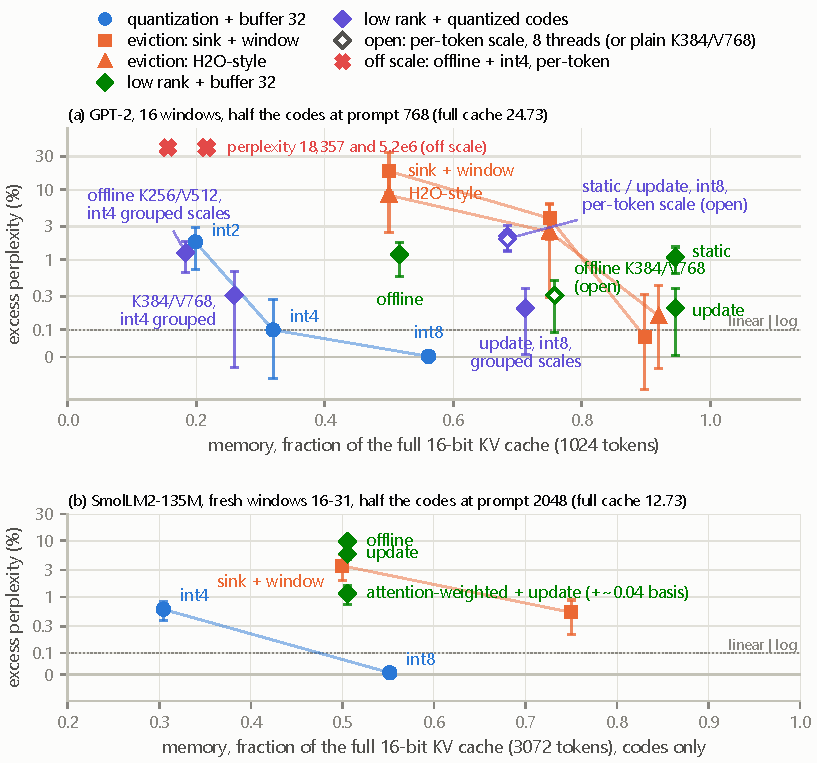
\includegraphics[width=0.9\textwidth]{figures/short_frontier.pdf}
\caption{Memory against excess perplexity (increase over the full cache; vertical axis linear below the dotted line at $0.1\%$, logarithmic above). Bars: paired 95\% bootstrap intervals over the 16 test windows; in (a) the cells at memory $0.92$ are shifted sideways by up to $0.022$ so that they do not overlap. (a) GPT-2, windows 0--15, half the codes, prompt 768 (C5 and C16: \texttt{c5\_kv\_baselines.json}, \texttt{c16\_kv\_quantlr.json}). Memory is relative to a 16-bit full cache at 1024 tokens and counts codes, scales, the exact first token and buffer and, for the online low-rank cells, the per-prompt basis. Open diamonds: per-token scale on the quantized low-rank codes (one 8-thread run, C16), and the unquantized offline K384/V768 cell. Red crosses: offline basis + 4-bit codes with a per-token scale (perplexity $18{,}357$ at ranks 256/512, $5{,}159{,}065$ at 384/768), far off the scale. The two 4-thread C5 cells with 8-bit low-rank codes ($+1.76\%$ at $0.28$, $+2.54\%$ at $0.68$) are omitted: compounded-quantization numbers depend on the thread count, so they are not comparable with C16. (b) SmolLM2-135M, fresh windows 16--31, prompt 2048 (C15; \texttt{c15b\_rope\_baselines\_w16-31.json}). Memory at 3072 tokens counts the stored codes only; the per-prompt basis would add about $0.04$ to the online low-rank cells.}
\label{fig:short-frontier}
\end{figure}

\begin{table}[!htb]
\centering\small
\begin{tabular*}{\textwidth}{@{\extracolsep{\fill}}lrrr@{}}
\toprule
method & copy top-1 & first difference (median) & KL per step\\
\midrule
full cache & 0.927 & 128 & 0\\
update + buffer 32 & 0.924 & 119 & 0.0010\\
static + buffer 32 & 0.918 & 58 & 0.0070\\
static, no buffer & 0.905 & 13 & 0.0189\\
offline + buffer 32 & 0.925 & 7 & 0.0112\\
offline, no buffer & 0.922 & 9.5 & 0.0188\\
\bottomrule
\end{tabular*}
\caption{Copy probe and greedy generation (\texttt{c6\_kv\_probe.json}; half the codes, $P=768$, 16 windows). ``Copy top-1'': share of the second copy of 128 random tokens predicted correctly. ``First difference'': index of the first of 128 greedily generated tokens that differs from the full model's (at least 1 by construction). ``KL per step'': mean Kullback--Leibler divergence of the next-token distribution from the full model's, on the full model's text.}
\label{tab:fu-probe}
\end{table}

\begin{figure}[!tbp]
\centering
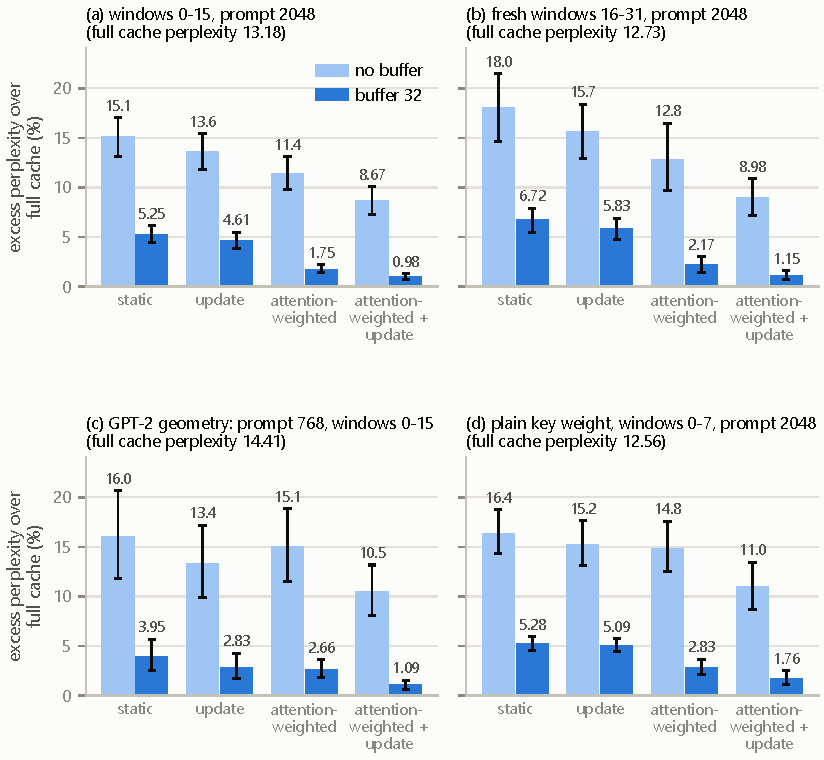
\includegraphics[width=0.9\textwidth]{figures/short_smollm.pdf}
\caption{SmolLM2-135M (rotary positions, grouped-query attention): excess perplexity over the full cache, one basis per layer, keys of rank 64 and values of rank 128 (half of the 192 numbers per token). Light bars: no buffer; dark bars: block buffer of 32 exact tokens. Static: basis from the prompt; update: refreshed every 32 tokens; attention-weighted: prompt rows weighted by the attention they receive (attn-late); attention-weighted + update: both, the new block rows entering the update unweighted (chosen post hoc). (a) Windows 0--15, prompt 2048, 1024 continuation tokens (\texttt{c13\_summary.json}, pooling \texttt{c11\_rope\_smollm2.json} and the \texttt{c13} runs; paired ratios in Table~\ref{tab:fu-rope}); (b) fresh windows 16--31 (C15, \texttt{c15a\_rope\_w16-31.json}); (c) prompt 768 and 255 continuation tokens as in GPT-2, windows 0--15 (C14, \texttt{c14a\_smollm2\_gpt2geom.json}); (d) the identity as key weight instead of the approximate query weight $G_K$, windows 0--7 (C14, \texttt{c14b\_smollm2\_plainK.json}). Error bars: 95\% paired bootstrap intervals over windows, stored in the summaries for (b)--(d), recomputed for (a) from the stored per-window log-likelihoods. With 2048-token prompts the stored codes take $0.505$ of the full cache at 3072 tokens, $0.548$ with the per-prompt basis (computed from Proposition~\ref{prop:kvmem}, not measured).}
\label{fig:short-smollm}
\end{figure}

\begin{table}[!htb]
\centering\small
\begin{tabular*}{\textwidth}{@{\extracolsep{\fill}}lr@{}}
\toprule
SmolLM2, windows 0--15: ratio of perplexities & 95\% CI (16 of 16 windows each)\\
\midrule
update / static, buffer 32 & $0.9939$ ($0.9921$--$0.9956$)\\
attn-late / static, no buffer; buffer 32 & $0.9680$ ($0.9604$--$0.9749$); $0.9667$ ($0.9606$--$0.9725$)\\
attn-late / update, buffer 32 & $0.9726$ ($0.9665$--$0.9784$)\\
attn-late + update / attn-late, buffer 32 & $0.9924$ ($0.9903$--$0.9942$)\\
attn-late + update / update, buffer 32 & $0.9653$ ($0.9588$--$0.9717$)\\
attn-late + update / attn-late, no buffer & $0.9754$ ($0.9704$--$0.9801$)\\
\bottomrule
\end{tabular*}
\caption{Paired perplexity ratios for panel (a) of Figure~\ref{fig:short-smollm} (\texttt{c13\_summary.json}; full cache $13.18$); a ratio below 1 means the first method is better. Pre-RoPE keys; approximate query weight. Checks: block-by-block full cache equals one pass to $7.6\times10^{-5}$; rotating keys back recovers them to $1.4\times10^{-6}$.}
\label{tab:fu-rope}
\end{table}

\subsection{Why the models differ, quantized codes, and controls}
\label{sec:kvround3}

Five more planned experiments, C14--C18 (named after their result files), address questions left open above; their rules and verdicts are in Table~\ref{tab:rules2}. Where a rule name was already used, the experiment number is put in front: \rl{C14-G1} is not the \rl{G1} of Section~\ref{sec:recipe}. ``Excess'' is the perplexity increase over the full cache on the same text; intervals are paired bootstrap 95\% intervals over the test windows. $R/n$ is the rank of a basis divided by the number of prompt rows it was fitted to, and \emph{attn-late} is the attention-weighted prompt basis of Section~\ref{sec:kvattn}.

\begin{figure}[!tb]
\centering
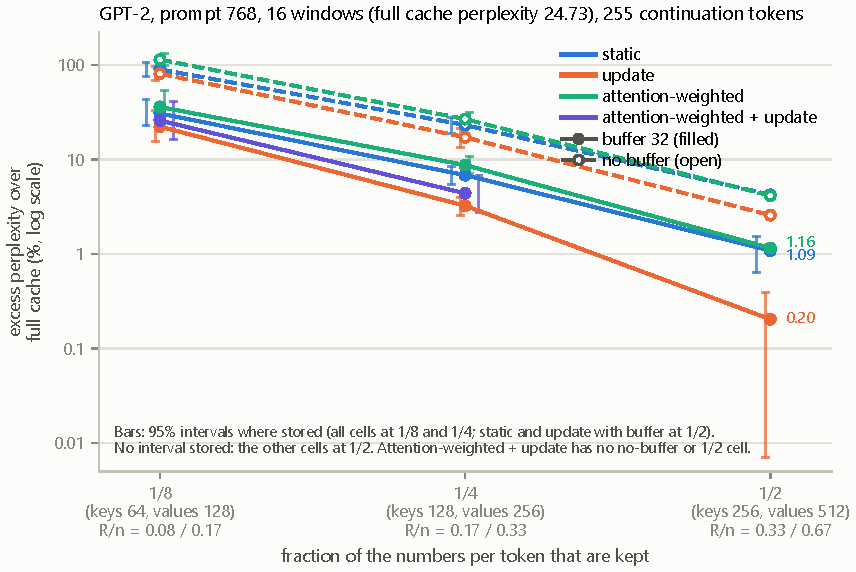
\includegraphics[width=0.9\textwidth]{figures/short_lowr.pdf}
\caption{GPT-2 at a lower rank-to-prompt ratio $R/n$ (C14; \texttt{c14c\_kv\_lowrn.json}, \texttt{c14c\_kv\_lowrn\_K128V256.json}): excess perplexity (log scale) against the fraction of the numbers per token kept. Prompt 768, windows 0--15, full cache $24.73$, 255 continuation tokens. Solid lines, filled markers: buffer 32; dashed lines, open markers: no buffer. Key/value ranks 64/128, 128/256 and 256/512 ($R/n$ $0.083/0.167$, $0.167/0.334$, $0.33/0.67$). The $1/2$ column repeats Sections~\ref{sec:kvbuffer} and~\ref{sec:kvattn}; attention-weighted + update was run only with the buffer at $1/8$ and $1/4$. Bars: stored 95\% bootstrap intervals (\texttt{c14\_summary.json} for $1/8$ and $1/4$; \texttt{c16\_summary.json} for static and update with the buffer at $1/2$); the other cells at $1/2$ have none.}
\label{fig:short-lowr}
\end{figure}

\paragraph{Why do GPT-2 and SmolLM2 differ? (C14).} On SmolLM2 attention weighting helped and the update helped little; on GPT-2 it was the reverse. The runs differ in $R/n$ (SmolLM2 keys: rank 64 on 2047 prompt rows, $0.03$; GPT-2: rank 256 on 767 rows, $0.33$), in prompt and continuation lengths, and in the model (rotary positions, grouped heads, an approximate pre-RoPE query weight). Three runs separate these (Figures~\ref{fig:short-lowr} and~\ref{fig:short-smollm}(c, d)). \emph{GPT-2 at a low $R/n$} (keys 64, values 128: $R/n=0.083$ and $0.167$, an eighth of the numbers) breaks the model, from $+22.29\%$ (update, buffer) to $+114.15\%$ (attn-late, no buffer). With the buffer static costs $+30.75\%$, the update $+22.29\%$ and attn-late $+36.05\%$ (ratio attn-late/static $1.040$, CI $1.009$--$1.080$; \rl{L1} fails). At a quarter (keys 128, values 256; buffer) the update costs $+3.25\%$, static $+6.84\%$, attn-late $+8.75\%$; against static the update has ratio $0.966$ (CI $0.957$--$0.975$, 16 of 16 windows) and attn-late $1.018$ (CI $1.005$--$1.036$; \texttt{c14\_summary.json}, key \texttt{c14c\_gpt2\_lowrn\_K128V256}). A low $R/n$ alone does not make weighting useful on GPT-2. \emph{SmolLM2 with GPT-2's geometry} (prompt 768, 255 new tokens, same ranks; with the buffer static $+3.95\%$, update $+2.83\%$, attn-late $+2.66\%$, attn-late + update $+1.09\%$): the update's ratio of excess to static falls from $0.878$ to $0.718$ (CI $0.616$--$0.792$), an $18\%$ larger relative gain where the rule asked for a quarter, and weighting still helps (ratio $0.673$, CI $0.559$--$0.832$, against $0.333$ in the main geometry); \rl{C14-G1} fails. \emph{A plain key weight on SmolLM2} (the identity instead of the approximate $G_K$; windows 0--7): attn-late with the buffer costs $+2.83\%$ against $+1.71\%$ with $G_K$ (ratio $1.011$, CI $1.007$--$1.015$, worse in 8 of 8 windows), static $+5.28\%$. Weighting keeps $68\%$ of its gain (\rl{C14-K1} fails): it works without the approximate query weight, only less well. Prompt length and $R/n$ explain part of the difference between the models, not all of it.

\paragraph{Fresh SmolLM2 windows, with baselines (C15).} The best SmolLM2 cell, attn-late + update with the buffer ($+0.98\%$), was chosen post hoc. On new windows 16--31 (Figures~\ref{fig:short-smollm}(b) and~\ref{fig:short-frontier}(b)) it costs $+1.15\%$ (CI $0.74$--$1.57\%$) against $+5.83\%$ ($4.72$--$6.89\%$) for the update and $+6.72\%$ for static (ratio of excess $0.197$, CI $0.133$--$0.265$, better in 16 of 16 windows): confirmed (\rl{C15-R1} passes). Without a buffer all four methods cost $+8.98\%$ to $+18.02\%$. Two results differ from GPT-2. The offline basis is clearly worse than the updated prompt basis, $+9.68\%$ ($8.66$--$10.69\%$; difference $3.85$ points, CI $3.03$--$4.80$, 16 of 16 windows; \rl{C15-R3} fails), worse even than static, whereas on GPT-2 offline and static were close ($+1.19\%$, $+1.09\%$). And quantization is again the better use of memory (\rl{C15-R4} fails): 4-bit costs $+0.60\%$ ($0.38$--$0.83\%$) at $0.30$ of the memory (\rl{C15-R2} passes) and 8-bit $+0.009\%$ ($0.001$--$0.017\%$) at $0.552$, just above the rule's memory cut, against $+1.15\%$ for the best low-rank cell at $0.505$ for the codes (about $0.55$ with the per-prompt basis). Sink + window eviction costs $+3.58\%$ ($1.95$--$5.68\%$) at $0.50$ and $+0.53\%$ ($0.21$--$0.88\%$) at $0.75$. These SmolLM2 memories count codes, scales and exact tokens only.

\paragraph{Low rank with quantization (C16).} Section~\ref{sec:kvchecks} found that 8-bit codes cost the updated low-rank cache far more than the offline one, with two candidate causes. With a \emph{per-token scale} (one scale and offset per token over its $R$ codes), a coordinate with a small spread, such as a low-energy direction, is rounded almost to zero by the scale of the large coordinates; \emph{grouped scales} (one per coordinate over 32 consecutive tokens, as KIVI \cite{liu2024kivi} does for keys) avoid this. \emph{Compounding}: the update re-projects and re-rounds the old codes seven times in 256 tokens; a diagnostic variant keeps a float \emph{master copy} of every row (not counted in the memory) and quantizes only when the cache is read. Setting: GPT-2, half the codes, $P=768$, $B=32$, windows 0--15, full cache $24.73$, one 8-thread run (\texttt{c16\_kv\_quantlr.json}; Figure~\ref{fig:short-frontier}(a)). Both causes are real (\rl{QL1}, \rl{QL2} pass). With per-token scales the updated cache costs $+2.18\%$ (CI $1.33$--$3.09\%$, memory $0.68$), with the master copy $+0.91\%$ ($0.26$--$1.58\%$); static with 8-bit codes costs $+1.97\%$ ($1.34$--$2.61\%$), unquantized static $+1.09\%$ ($0.63$--$1.52\%$). Without the master copy the median relative error of the stored key codes grows from $0.019$ (no re-projection) to $0.057$ (seven), a factor $3.0$ ($2.9$ for values); with it the error stays flat (factors $1.06$ and $1.01$). \emph{Grouped scales remove the whole loss: $+0.203\%$ (CI $0.008$--$0.391\%$) at $0.71$ of the memory}, indistinguishable from the unquantized update ($+0.204\%$, $0.007$--$0.392\%$, at $0.92$; with the master copy $+0.205\%$; difference to per-token scales $-1.97$ points, CI $-2.80$ to $-1.21$). Removing the compounding alone (master copy) recovers $1.3$ of the $2.0$ points ($2.18\to0.91$); grouping the scales alone recovers all of them ($2.18\to0.20$), so the per-token scale is the root cause and re-rounding amplifies it.

\rl{QL3} (offline basis + 4-bit costs at most $1\%$) fails as written: with per-token scales the offline basis is catastrophic (perplexity $18{,}357$ at ranks 256/512 and $5{,}159{,}065$ at 384/768, memory $0.16$ and $0.22$). With grouped scales 4-bit codes cost nothing extra: $+1.26\%$ ($0.65$--$1.85\%$) at $0.18$ (ranks 256/512; unquantized $+1.19\%$, $0.57$--$1.78\%$, at $0.52$) and $+0.31\%$ ($-0.04$--$0.67\%$) at $0.26$ (ranks 384/768; unquantized $+0.31\%$, $0.09$--$0.51\%$, at $0.76$). That is competitive with, not better than, plain 4-bit quantization ($+0.109\%$, CI $-0.07\%$ to $+0.28\%$, at $0.32$); the intervals overlap. The same per-token 8-bit cell gave $+2.54\%$ at 4 threads (Section~\ref{sec:kvchecks}) and $+2.18\%$ here at 8 threads: rounding differences compound, so the two numbers are not comparable, and we compare quantized variants only within one run.

\begin{figure}[!tb]
\centering
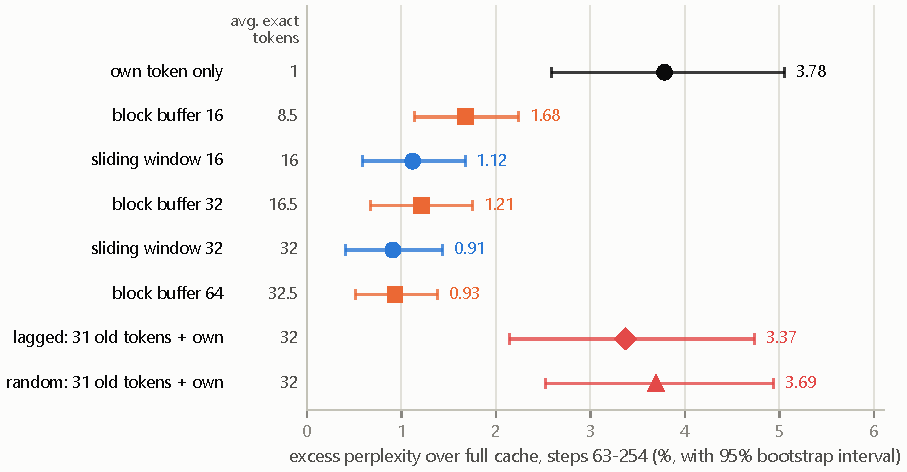
\includegraphics[width=0.9\textwidth]{figures/short_equalbudget.pdf}
\caption{Equal-budget recency controls on a static basis (GPT-2, half the codes, $P=768$, windows 0--15; \texttt{c18a\_kv\_equalcount.json}, \texttt{c18\_summary.json}). Excess perplexity, scored on continuation steps 63--254 (192 of 255) so that no method is penalised by the budget ramp of the recency controls; bars: 95\% bootstrap intervals over windows. Second column: average number of exact tokens (a block buffer of size $B$ holds $(B+1)/2$ on average, a sliding window always its full size). Lagged: own token plus 31 continuation tokens of age 32--62; random: own token plus 31 random continuation tokens older than 32 (intervals recomputed from the stored per-step log-likelihoods). Only recency of the exact tokens helps.}
\label{fig:short-equalbudget}
\end{figure}

\paragraph{AttSVD's accumulating mode (C17).} Weighting failed on GPT-2 because the error that attention reads sits on new tokens (Section~\ref{sec:kvattn}). AttSVD \cite{attsvd2026} keeps new tokens exact in its main \emph{accumulating mode} and compresses only the prompt, once, with a static basis. Weighting gives nothing there either (\rl{C17-A1} fails; \texttt{c17\_kv\_accum.json}): unweighted $+0.140\%$, attn-late $+0.162\%$ (ratio $1.0002$, CI $0.9991$--$1.0014$); with the 384-token prompt and keys only, $+0.011\%$ and $+0.026\%$ (ratio $1.0002$, CI $0.9998$--$1.0005$). This mode does not reconcile our result with AttSVD, and there is little to gain: the compressed prompt alone costs $0.14\%$.

\paragraph{Sliding window or block buffer at equal budget (C18a).} A block buffer of size $B$ holds on average $(B+1)/2$ exact tokens, a sliding window of 32 always 32, so the earlier comparison favoured the window. At equal average budget, scored from continuation step 63 on (192 of 255 steps, which also removes the budget ramp of the recency controls), the two are not resolved (Figure~\ref{fig:short-equalbudget}): sliding 16 costs $+1.12\%$ against $+1.21\%$ for block 32 (ratio $0.9991$, CI $0.9952$--$1.0027$), sliding 32 $+0.91\%$ against $+0.93\%$ for block 64 (ratio $0.9998$, CI $0.9970$--$1.0021$). \rl{C18-E1} and \rl{C18-E2} pass as written, but the window's earlier advantage (Section~\ref{sec:kvbuffer}) came from its larger budget. Over all steps the own token alone, sliding 16 and 32 and block 16, 32 and 64 cost $+3.47\%$, $+0.95\%$, $+0.77\%$, $+1.55\%$, $+1.09\%$ and $+0.79\%$: the same ranking. Recency also survives the ramp-free scoring. Rule \rl{Z3} predicted that 31 lagged old tokens (ages 32--62) plus the own token would recover at least half of the sliding window's gain over the own token alone, that is, cost at most $2.35\%$; it fails. The lagged control costs $+3.37\%$ and 31 random old tokens $+3.69\%$, against $+3.78\%$ (CI $2.59$--$5.05\%$) for the own token alone and $+0.91\%$ for sliding 32; the lagged control lies $1.0$ point above the threshold (CI $0.20$ to $1.88$). Exact old tokens do not help like exact recent ones.

\paragraph{Out-of-sample error or drift of the text? (C18b).} The held-out check of Section~\ref{sec:blockscheme} fitted the first half of the prompt and tested on the second, which comes later in the text, so slow drift could mimic out-of-sample error. Fitting a random interleaved half of the prompt rows instead (\texttt{c18b\_kv\_novelty\_interleaved.json}; medians of the residual ratios) lowers the held-out ratio from $3.21$ to $1.72$ for keys ($-47\%$) and from $5.60$ to $4.11$ for values ($-27\%$): \rl{N4} (no drift) fails. The continuation ratios fall too (keys $4.27\to2.19$, values $5.88\to4.75$). As excess over 1, drift is about two thirds of the keys' gap ($2.21\to0.72$) and a third of the values' ($4.60\to3.11$). The rest, $1.72$ and $4.11$, is out-of-sample error proper, close to the Gaussian model's $1.63$ and $3.38$ (computed for a different fit, so the comparison is rough).

\means Four earlier readings change. (1) The gap between new and fitted tokens is out-of-sample error \emph{plus drift of the text}, drift mattering most for keys. (2) At equal budget a sliding window is not shown to beat a block buffer, and recency still matters without the ramp. (3) Attention weighting does not help GPT-2, neither with exact new tokens nor at a lower $R/n$ (there it hurts); it helps SmolLM2, less at a short prompt or with a plain key weight. So the models differ by more than $R/n$ or prompt length. (4) The 8-bit loss on an updated basis has its root in the per-token scale, and re-rounding the old codes at every update amplifies it; with grouped scales the low-rank cache is quantized without loss ($+0.20\%$ at $0.71$ of the memory). Low rank still does not beat plain 4-bit quantization, on GPT-2 or on SmolLM2. Open: long contexts (SmolLM2 at 4--8k tokens), a retrieval test such as passkey, and a model larger than 135 million parameters.


\subsection{Sinks, heads, domain shift and additivity over layers}
\label{sec:kvadditive}

Five more planned experiments return to questions of earlier sections: whether the sink geometry of Section~\ref{sec:sink} carries over to SmolLM2 (C19), why keeping the first key exact hurts the plain basis on GPT-2 (C20, also Section~\ref{sec:sink}), whether one basis per layer beats one per head on SmolLM2 as on GPT-2 (C21, Sections~\ref{sec:option2} and~\ref{sec:groups}), what an offline basis calibrated on the wrong kind of text costs against the prompt basis (C22, Sections~\ref{sec:kvonline} and~\ref{sec:blockscheme}), and whether errors add up over layers, as the one-layer bounds of Section~\ref{sec:kvbound} implicitly assume (C23). Rules and verdicts are in Table~\ref{tab:rules2}. All five use 8 test windows, so the intervals are wide.

\paragraph{Sink check on SmolLM2 (C19).} SmolLM2 has 30 layers and 3 key--value heads of size 64. For each key--value head we fitted a basis of rank 16, 32 or 48 (of 64) on the keys \emph{before} RoPE, in the four variants of Section~\ref{sec:sink}: plain (second moment of the keys), centered (mean removed, so the basis cannot represent it), each also with the first key stored exactly (``keep0''); windows 0--7, dense perplexity $20.074$ (\texttt{c19\_rope\_sink.json}). Perplexities at ranks 16/32/48: plain $39.30$/$27.20$/$22.37$; plain keep0 $33.38$/$22.72$/$21.10$; centered $171.15$/$26.51$/$22.04$; centered keep0 $32.15$/$22.10$/$20.62$. The GPT-2 geometry does not carry over: the first key's coordinate along the mean direction, $k_0\cdot\hat\mu$, is negative in only 16 of 30 layers (\rl{C19-S1} fails; median $-0.01\lVert\mu\rVert$), positive in layers 0--11 ($0.20$ to $1.09$) and within about $\pm0.1$ of zero in layers 12--29. Those upper layers hold the sink: 18 of 30 layers, namely 12--29, put at least $30\%$ of their attention on position 0 ($0.30$ to $0.67$), layers 0--11 only $0.00$ to $0.09$. Centered/plain perplexity ratios are $4.35$ (CI $3.68$--$5.12$, worse in 8 of 8 windows), $0.975$ ($0.946$--$1.009$) and $0.985$ ($0.977$--$0.993$): centering is catastrophic only at rank 16 (\rl{C19-S2} fails). Keep0 rescues the centered basis at every rank (\rl{C19-S3} passes) and, unlike on GPT-2, also \emph{improves} the plain one: ratios plain keep0/plain $0.849$ ($0.796$--$0.928$), $0.835$ ($0.811$--$0.861$) and $0.943$ ($0.931$--$0.956$) (\rl{C19-S4}, which expected harm, fails). Centered keep0/plain keep0 is $0.963$, $0.973$ and $0.977$ (intervals within $0.956$--$0.985$, below 1 in 8 of 8 windows at each rank; \rl{C19-S5} passes). In a dense pass (windows 0--3, rank 32, median over layers) the score error on position 0 is $1.55$ logits for the plain basis and $1.95$ for the centered one, against $0.40$ and $0.38$ for the other keys. So the sink matters on SmolLM2 and storing it exactly helps every basis, but not through the GPT-2 geometry. Caveats: one small RoPE model, 8 windows, pre-RoPE keys, and a post-RoPE score error approximated per key--value head with the query heads of its group.

\paragraph{Why does keep0 hurt the plain basis on GPT-2? (C20).} Section~\ref{sec:sink} found that storing the first key exactly makes the \emph{plain} basis worse on GPT-2. The tested explanation was cancellation: a compressed first key's score error partly cancels those of the other keys (a common shift of all scores leaves the softmax unchanged), and keeping it exact removes the cancellation. The harm is resolved at rank 32 only: $70.585\to73.246$, ratio $1.038$ (CI $1.019$--$1.058$; keep0 better in 1 of 8 windows), while at rank 16 $310.656\to317.290$ gives ratio $1.021$ (CI $0.989$--$1.055$; 4 of 8), so \rl{C20-H0} (replication at both ranks) fails. Compressing one layer at a time (rank 16) puts almost all of the harm in layer 0 ($+0.0992$ nats per token, i.e.\ natural-log loss per token; an excess of $x$ nats multiplies perplexity by $e^x$), then layer 10 ($+0.0079$) and layer 7 ($+0.0038$); the others are at most $+0.0004$ or slightly negative (down to $-0.0030$). Layer 0 gives position 0 almost no attention (mean $0.006$), so this is not a sink effect in the usual sense. The layers also interact: layer 0 alone costs $+0.099$ nats per token, all layers together $\ln(317.29/310.656)=+0.021$. Cancellation is not supported: a per-layer cancellation measure correlates with the single-layer harm at Spearman $0.469$ (\rl{C20-H1} needed $0.6$; the signs agree in 9 of 12 layers), and the first key's attention-weighted error is smaller than the other keys' in 8 of 12 layers (\rl{C20-H2} needed 9). Why keep0 hurts the plain basis on GPT-2 remains unexplained.

\paragraph{One basis per layer or per head on SmolLM2 (C21).} On GPT-2 one basis shared by the heads of a layer beat one basis per head at equal memory (Sections~\ref{sec:option1} and~\ref{sec:option2}). SmolLM2 has only 3 key--value heads, so ``per head'' means three bases per layer. At equal stored numbers per token and layer (192: keys 64 and values 128 per layer, about 21 and 43 per head after rounding; 2048-token prompts, windows 0--7; \texttt{c21\_summary.json}), the per-layer basis is better in 8 of 8 windows in all three settings (\rl{C21-PH1} to \rl{C21-PH3} pass; sign test $p=0.0078$). Perplexity ratios per head/per layer: $1.122$ (CI $1.085$--$1.165$) for static with the buffer ($+18.15\%$ against $+5.33\%$), $1.129$ ($1.091$--$1.174$) for the update with the buffer ($+18.14\%$ against $+4.60\%$), and $1.347$ ($1.270$--$1.423$) for static without buffer ($+56.96\%$ against $+16.49\%$). The GPT-2 finding replicates on a model with rotary positions and grouped-query attention, with a larger gap. The per-head bases need a third of the basis numbers ($12{,}288$ against $36{,}864$ per layer), which does not offset the loss. Caveats: with 3 key--value heads ``per head'' is a coarse split; rounded per-head ranks; 8 windows.

\paragraph{Calibration on another kind of text (C22).} The offline basis of Section~\ref{sec:recipe} is fitted on WikiText calibration text, the prompt basis on the text being read. We measured the cost of calibrating on the wrong domain (GPT-2 main setting, buffer 32 throughout). The second domain is children's stories (TinyStories validation split: calibration from its first 6 million characters, targets from characters 6 to 8 million), a mild shift in register. ``Matched'' means calibrated on the target's own domain, ``mismatched'' on the other. Table~\ref{tab:c22} gives the excess of each basis on both targets.

\begin{table}[!htb]
\centering\small
\begin{tabular*}{\textwidth}{@{\extracolsep{\fill}}lrr@{}}
\toprule
basis (buffer 32) & wiki target (full cache $24.140$) & story target (full cache $9.794$)\\
\midrule
offline, matched & $+1.12\%$ ($0.06$--$2.18$) & $+0.58\%$ ($-0.36$--$1.85$)\\
offline, mismatched & $+8.28\%$ ($6.51$--$10.20$) & $+2.39\%$ ($-0.92$--$5.91$)\\
prompt basis, static & $+1.11\%$ ($0.49$--$1.76$) & $+0.96\%$ ($0.09$--$1.79$)\\
prompt basis, update & $+0.25\%$ ($0.03$--$0.45$) & $+0.04\%$ ($-0.25$--$0.36$)\\
offline matched + update & $+0.67\%$ ($-0.02$--$1.34$) & $+0.18\%$ ($-0.51$--$1.14$)\\
offline mismatched + update & $+4.72\%$ ($3.25$--$6.31$) & $+1.20\%$ ($-0.54$--$3.17$)\\
\bottomrule
\end{tabular*}
\caption{Calibration on another kind of text (C22; GPT-2, half the codes, $P=768$, windows 0--7 of each target; \texttt{c22\_kv\_domainshift.json}). Excess perplexity over the full cache, with 95\% bootstrap intervals in percentage points.}
\label{tab:c22}
\end{table}

On the wiki target the mismatch clearly costs more (perplexity ratio $1.071$, CI $1.057$--$1.085$, 8 of 8 windows); on the story target the ratio, $1.018$ (CI $0.982$--$1.055$), is not resolved, so \rl{C22-D1} fails. The updated prompt basis is no worse than the mismatched offline basis on both targets (\rl{C22-D2} passes) and indistinguishable from the matched one (ratios $0.991$, CI $0.982$--$1.002$, and $0.995$, CI $0.984$--$1.003$). Updating a mismatched offline basis roughly halves its loss (\rl{C22-D3} passes) but does not remove it. So the prompt basis is as good as an offline basis fitted to the right domain, without having to know the domain, and much better than one fitted to the wrong domain. Caveats: one asymmetric shift (stories are easy, so their intervals are wide); 8 windows; calibration on 16 windows of 1024 tokens; the severity of the mismatch was not controlled.

\paragraph{Additivity over layers (C23).} The bounds of Section~\ref{sec:kvbound} treat one attention operation at a time, and the per-layer experiments of Section~\ref{sec:kv} measure one layer with the others exact; both reason as if the loss added up over layers. We tested this on GPT-2 with the offline per-layer basis of Section~\ref{sec:recipe} (keys 256, values 512, shared by the 12 heads of a layer, query-aware keys, output-aware values, first token \emph{not} kept exact), in full 1024-token passes on windows 0--7, compressing only the layers in a subset $S$ (no layer: the dense loss exactly; all 12: perplexity $34.979$ against $33.644$). Let $d(S)$ be the excess loss over the dense model in nats per token and $s(S)$ the sum of the single-layer excesses of the layers in $S$; if excess were additive, $d(S)/s(S)$ would be 1. Over 171 subsets (12 single layers, all 66 pairs, 30 random triples, 20 random subsets each of size 4, 6 and 8, the two halves, even and odd layers, all 12): all 12 layers give $d=0.03892$ against $s=0.02484$, a ratio of $1.57$ (window-bootstrap CI $1.43$--$1.84$), so \rl{C23-A1} (ratio within $0.2$ of 1) fails. The median $|d/s-1|$ over the 60 random subsets is $0.217$ (\rl{C23-A2} needed at most $0.20$; it fails narrowly), and it grows with the subset size: $0.118$, $0.168$ and $0.263$ for 4, 6 and 8 layers, with median ratios $1.065$, $1.168$ and $1.263$. Pairs are close to additive (median pair interaction $0.062$ of the two singles' sum; \rl{C23-A3} passes), and $57.6\%$ of the pairs are super-additive (cost more together than apart). Named subsets: layers 0--5 $2.13$ ($d=0.00233$, $s=0.00109$), layers 6--11 $1.35$ ($0.03215$, $0.02375$), even layers $1.15$ ($0.01220$, $0.01061$), odd layers $1.08$ ($0.01531$, $0.01423$).

\means Excess loss is roughly additive for a few layers and super-additive for many, plausibly because a layer reads inputs that earlier compressed layers have already distorted. Summed per-layer errors, or one-layer-at-a-time bounds, therefore \emph{underestimate} the cost of a full model, by roughly $20\%$ at 6 layers and $50\%$ at 12 in this setting; the rankings of Section~\ref{sec:kvbound} still stand, but their sizes should not be summed. Caveats: the single-layer excesses are tiny (at most $0.0098$ nats, $1\%$ in perplexity; four are slightly negative, that is, noise), so ratios of small subsets, in particular the first six layers ($2.13$), rest on denominators near the noise level; one model, one rank setting, 8 windows, and only \rl{C23-A1} has a confidence interval. Of the other results of this subsection, two GPT-2 findings carry over to SmolLM2 (one basis per layer beats one per head; the first token matters), while the sink geometry does not; the keep0 harm on GPT-2 sits in layer 0 and remains unexplained; and a prompt basis is as good as an offline basis calibrated on the right domain.

% =====================================================================

% ---- end short/s08b_followups ----
% ---- begin short/s09_discussion ----
\section{Discussion and conclusion}
\label{sec:discussion}
% =====================================================================

\subsection{What is known and what is new}
\label{sec:novelty}

A literature check made after the experiments (Section~\ref{sec:relwork}) found much of what we built already published, mostly on models about 65 times larger than GPT-2 small: activation-aware SVD of the weights and the lesson that output error matters more than weight error \cite{wang2025svdllm,yuan2023asvd,hsu2022}; bases per head, per group and per layer \cite{palu2025}; query-aware keys \cite{attsvd2026,saki2026} and an optimal low-rank factorization of the attention scores \cite{kqsvd2025} (we did not check whether KQ-SVD also weights the values by $W_O$); a per-prompt basis without calibration data \cite{attsvd2026}, and a prompt basis shared by the heads of a layer, updated by Brand's incremental SVD with an exact recent window \cite{iskv2026} or by Oja's rule \cite{ojakv2025}; exact sink tokens \cite{xiao2024sinks,ojakv2025}, and low-rank keys losing the sink token \cite{saki2026}; methods that control the attention-output error \cite{readkv2026,anchorkv2026} (only parts read); and related designs \cite{saxena2024eigen,sun2024shadowkv,chang2025xkv,liu2024minicache,zhang2024lorc,ji2025mha2mla,meng2025transmla}. The chi-squared step of Proposition~\ref{prop:attnout3} is classical.

Our KV recipe is therefore \emph{independently reached, close to iS-KV and AttSVD}. What we did not find elsewhere is the analysis:
\begin{enumerate}[leftmargin=2em,itemsep=0pt]
\item a planned test that separates the two ingredients of the updated cache, the exact recent buffer and the basis update; follow-ups show that the exact tokens that matter are the newest ones, because they are recent (a control with older continuation tokens fails), not because of the attention they receive (Sections~\ref{sec:blockscheme} and~\ref{sec:kvbuffer});
\item an ``oracle'' comparison and a measurement showing that new tokens fit the basis worse than the prompt it was fitted to, by a factor that stays roughly constant once the basis is updated; the gap is partly out-of-sample error and partly drift of the text over time (an interleaved held-out split cuts the keys' excess over 1 by about two thirds; Sections~\ref{sec:blockscheme} and~\ref{sec:kvround3});
\item on GPT-2, weighting the prompt basis by the attention each token receives does not help when new tokens are compressed too, because almost all of the error that attention reads sits on new tokens (Section~\ref{sec:kvattn}); it does not help either when new tokens are kept exact, and a lower rank-to-prompt ratio makes it worse (Section~\ref{sec:kvround3}); on a small rotary-position model it did help, so the result depends on the model, and prompt length and rank explain only part of the difference (Sections~\ref{sec:kvchecks} and~\ref{sec:kvround3});
\item the geometry behind the ``attention sink'': the first token's key lies on the opposite side of the origin from the mean key, consistent with a mean-removing basis pulling it the wrong way (Section~\ref{sec:sink}; confirmed on 16 windows). Keeping the first key exact (keep0) makes the plain basis slightly worse on GPT-2 (resolved at rank 32 only, concentrated in layer 0); the harm stays unexplained (a cancellation explanation failed, C20); adding the mean direction to a centered basis does not replace keep0 (\rl{K1}). On SmolLM2 the geometry does not carry over, though the sink still matters (Section~\ref{sec:kvadditive});
\item measurements of how tight attention-weighted bounds on the attention output are on real attention, and why; only the tightest ranks the bases better than a trivial proxy (Section~\ref{sec:kvbound}).
\end{enumerate}
These could support an analysis paper, not a methods paper, and only after the extensions of Section~\ref{sec:future}. The equal-memory comparison (Section~\ref{sec:kvchecks}) also shows that, on GPT-2, the low-rank cache is not the best use of memory.

\subsection{Limitations}
\label{sec:limits}
\begin{itemize}[leftmargin=2em,itemsep=1pt]
\item \emph{One small model.} Almost everything was measured on GPT-2 small (1024 tokens of context, no RoPE). Newer models rotate keys by position, so a shared key basis must work before the rotation, and their heads are larger. The port to SmolLM2-135M (Section~\ref{sec:kvchecks}; one small RoPE model, 8--16 windows, no 4--8k-token contexts) changed two conclusions: the updated basis costs $+4.6\%$ instead of $+0.2\%$, and attention weighting helps ($+0.98\%$ with the update; $+1.15\%$ on fresh windows). Why the models differ is only partly explained (Section~\ref{sec:kvround3}).
\item \emph{One quality measure.} WikiText-2 perplexity on $8192$ test tokens (plus $8192$ for confirmation; 4080 continuation tokens in Sections~\ref{sec:kvonline}--\ref{sec:kvupdate}), with no task benchmarks and no retraining. A copy probe and greedy generation (Section~\ref{sec:kvchecks}) are the only other checks.
\item \emph{Short prompts and continuations.} Prompts are short for a 512-direction basis. On GPT-2 the updated basis saw continuations of at most 768 tokens (after the 256-token prompt of Section~\ref{sec:blockscheme}); on SmolLM2, 1024.
\item \emph{CPU timing only.} Single-sequence CPU timings with plain PyTorch operations. The update was timed on its own, next to a decode step, not inside a generation loop with a factored cache. The GPU expectation of Section~\ref{sec:timing} is not measured. The timing applies to GPT-2's absolute positions only: with RoPE the key basis cannot be folded into the query, and with grouped-query attention the arithmetic factor differs. Absolute times vary between sessions (Appendix~\ref{app:rerun}).
\item \emph{Scope of individual tests.} Regime B: two matrices, one $\lambda$, one mask and seed per cell. Regime C: one rank for all matrices of a given ratio, one RSVD draw. Groups of heads were consecutive only. Calibration and test text are both WikiText except one mild domain shift (children's stories, GPT-2, 8 windows, C22, Section~\ref{sec:kvadditive}; wide intervals on the story target; no code or other language). The query-aware weight assumes queries and keys are independent; the output-aware value weight is exact only per head (Section~\ref{sec:recipe}). The bounds cover one attention operation, not errors passed between layers: compressing all 12 layers costs $1.57$ times the sum of the single-layer excesses (Section~\ref{sec:kvadditive}), so the layer-by-layer reading underestimates the full model. The attention-weighted basis was tested only as a static prompt basis.
\item \emph{Memory and statistics.} The per-prompt basis costs memory that GPT-2's short texts cannot repay (memory $0.92$, Proposition~\ref{prop:kvmem}), and quantization uses memory better (Section~\ref{sec:kvchecks}). Confidence intervals exist only for the follow-up experiments (Sections~\ref{sec:kvchecks}--\ref{sec:kvadditive}) and the repeats of Sections~\ref{sec:blockscheme}--\ref{sec:kvattn} on fresh windows 16--31; other results use 16 windows (8 in Section~\ref{sec:kv}) and one RSVD seed, without intervals. With 16 windows, paired intervals resolve a few tenths of a percent at best, and the many comparisons are not corrected for multiple testing. Sections~\ref{sec:kvonline}--\ref{sec:kvupdate} reuse test windows 0--15, and the pair K256/V512 and the exact first token were chosen after seeing windows 0--7.
\item \emph{Design confounds.} The ``buffer'' is the current block, so on average only about $B/2$ recent tokens are exact, and block size, buffer size and update period are one parameter (a sliding window of 32 gives $+0.77\%$ against $+1.09\%$ with about twice as many exact tokens; at equal average budget the two are not resolved, Section~\ref{sec:kvround3}). ``No buffer'' compresses a token's own key and value before its own attention reads them. Three cells of the buffer-or-update test were known beforehand (Section~\ref{sec:kvbuffer}). The offline statistics include each calibration window's first token, the online ones do not; leaving it out offline changes nothing ($25.371$ and $25.031$ against $25.368$ and $25.022$). The recency control of Section~\ref{sec:kvbuffer} has a budget ramp (no extra exact token in the first 32 steps, fewer than 31 until step 62; the conclusion survives scoring from step 63, Section~\ref{sec:kvround3}) and restores exact rows from a copy. Quantized variants depend on the thread count (one per-token 8-bit run gave $+2.54\%$ and $+2.18\%$), so they are compared only within a run. The combined attention-weighted and updated basis on SmolLM2 was chosen after seeing the first SmolLM2 result. The role of the short continuation in rules \rl{C3} and \rl{C4} is post hoc, and the explanations of the buffer synergy and of the out-of-sample gap were tested afterwards (Sections~\ref{sec:blockscheme} and~\ref{sec:kvbuffer}).
\end{itemize}

\subsection{Future work}
\label{sec:future}
\begin{itemize}[leftmargin=2em,itemsep=1pt]
\item \emph{A larger RoPE model on a GPU} (for example an 8-billion-parameter Llama or Qwen model, keys compressed before the rotation; the partial-RoPE step of MHA2MLA \cite{ji2025mha2mla} and the RoPE-aware covariance of SAKI-RoPE \cite{saki2026} are the closest recipes; Qwen2.5-0.5B \cite{qwen2025} is the next CPU step after SmolLM2). Repeat the buffer-or-update and attention-weighting tests there, compare with iS-KV, AttSVD, OjaKV and Palu at equal memory, evaluate on long-context benchmarks (LongBench, RULER), and time a real decode loop with a factored cache.
\item \emph{Low rank against quantization on larger models}, where the basis is amortized over long texts and grouped scales may change the comparison; on GPT-2 quantization wins (Sections~\ref{sec:kvchecks} and~\ref{sec:kvround3}).
\item \emph{Why GPT-2 and SmolLM2 differ}, beyond prompt length and rank (Section~\ref{sec:kvround3}): longer SmolLM2 continuations (4--8k tokens), passkey retrieval, a stronger domain shift (code, another language), and the side effect of keeping the first key exact on GPT-2 (cancellation excluded, located in layer 0; Section~\ref{sec:kvadditive}).
\item \emph{A cheaper update:} a rank-$n_{\mathrm{blk}}$ update of the eigendecomposition instead of refactoring the whole $(R+n_{\mathrm{blk}})\times(R+n_{\mathrm{blk}})$ core (Frequent Directions, Section~\ref{sec:kvcheap}, was not cheaper).
\item \emph{Lower priority:} groups of similar (not consecutive) heads; weight ranks chosen per layer by output error; theory for RSVD-started ALS.
\end{itemize}

\subsection{Conclusion}
\label{sec:conclusion}

The theory of Section~\ref{sec:theory} held on every real matrix we checked: the SVD was optimal, RSVD fast and nearly optimal, and ALS never increased its objective. But its probabilistic bounds were too loose to be informative on GPT-2's flat spectra, and its guarantees cover the matrix, not the model.

GPT-2's weights are not close to low rank. The best factorization by the textbook criterion breaks the model at 90\% of its size, ALS cannot recover pruned weights, and only a factorization chosen by the error on real inputs keeps the model usable. Output error is a better guide than weight error, though it does not compare models of different sizes.

The KV cache is not low rank head by head, but one weighted basis per layer halves it at $+4\%$ perplexity, for $6\times$ more attention arithmetic that a CPU cannot hide. A basis computed from the prompt, updated every 32 tokens, with the newest tokens and the sink token exact, costs $+0.2\%$ on GPT-2 while storing half the codes, with three caveats: it uses an exact SVD of the prompt ($+0.3\%$ with RSVD); on the small RoPE model SmolLM2 it costs $+4.6\%$, where an attention-weighted basis with the update does better ($+0.98\%$, post hoc; $+1.15\%$ on fresh windows); and on fresh text a larger exact buffer alone (128 tokens) does as well. Counting the per-prompt basis, it still needs $0.92$ of the full memory at 1024 tokens, and 8- or 4-bit quantization reaches the same quality at much lower memory. The planned tests suggest why the recipe works: new tokens fit the basis worse than the tokens it was fitted to, and they receive much of the attention; the buffer protects them because they are recent, and the update keeps the basis current for older text. Our bounds agree: to first order, errors count in proportion to the attention their tokens receive, and the variance form comes within a median $2.6\times$ of the actual error.

The recipe itself turned out to be known. What this report adds is a self-contained derivation from first principles and an analysis of why the recipe works that we did not find in the papers we checked.

% =====================================================================
\FloatBarrier

% ---- end short/s09_discussion ----
% ---- begin short/bib ----
{\small
\begin{thebibliography}{99}
\setlength{\itemsep}{0pt}
\bibitem{ainslie2023} J.~Ainslie et al., GQA: Training generalized multi-query transformer models from multi-head checkpoints, in \emph{EMNLP}, 2023.
\bibitem{allal2025smollm2} L.~Ben Allal et al., SmolLM2: When smol goes big -- data-centric training of a small language model, arXiv:2502.02737, 2025.
\bibitem{anchorkv2026} M.~Khalaf, Y.~Shamshoum, N.~Hodos, Y.~Sieradzki, and A.~Schuster, AnchorKV: Anchor-residual KV cache compression, arXiv:2608.02901, 2026.
\bibitem{attsvd2026} S.~Abdali, J.~Ko, and P.~Cameron, AttSVD: Prompt-adaptive low-rank KV cache compression via attention-guided SVD, arXiv:2610.06927, 2026.
\bibitem{brand2006} M.~Brand, Fast low-rank modifications of the thin singular value decomposition, \emph{Linear Algebra and its Applications} 415(1):20--30, 2006.
\bibitem{candesrecht2009} E.~J.~Cand\`es and B.~Recht, Exact matrix completion via convex optimization, \emph{Foundations of Computational Mathematics} 9(6):717--772, 2009.
\bibitem{chang2025xkv} C.-C.~Chang, W.-C.~Lin, C.-Y.~Lin, H.-Y.~Chiang, Y.~Akhauri, X.~Dai, H.~Jiang, Y.~Li, L.~Ceze, K.-C.~Wu, and M.~S.~Abdelfattah, xKV: Cross-layer KV-cache compression via aligned singular vector extraction, in \emph{ICML}, PMLR 306:12758--12778, 2026 (arXiv:2503.18893).
\bibitem{deepseek2024} DeepSeek-AI, DeepSeek-V2: A strong, economical, and efficient mixture-of-experts language model, arXiv:2405.04434, 2024.
\bibitem{eckartyoung1936} C.~Eckart and G.~Young, The approximation of one matrix by another of lower rank, \emph{Psychometrika} 1(3):211--218, 1936.
\bibitem{frantar2023gptq} E.~Frantar et al., GPTQ: Accurate post-training quantization for generative pre-trained transformers, in \emph{ICLR}, 2023.
\bibitem{funk2006} S.~Funk, Netflix update: Try this at home, blog post, 2006.
\bibitem{ghashami2016} M.~Ghashami, E.~Liberty, J.~M.~Phillips, and D.~P.~Woodruff, Frequent directions: Simple and deterministic matrix sketching, \emph{SIAM Journal on Computing} 45(5):1762--1792, 2016 (arXiv:1501.01711).
\bibitem{golubvanloan2013} G.~H.~Golub and C.~F.~Van Loan, \emph{Matrix Computations}, 4th ed., Johns Hopkins University Press, 2013.
\bibitem{grippo2000} L.~Grippo and M.~Sciandrone, On the convergence of the block nonlinear Gauss-Seidel method under convex constraints, \emph{Operations Research Letters} 26(3):127--136, 2000.
\bibitem{halko2011} N.~Halko, P.-G.~Martinsson, and J.~A.~Tropp, Finding structure with randomness: Probabilistic algorithms for constructing approximate matrix decompositions, \emph{SIAM Review} 53(2):217--288, 2011.
\bibitem{han2016} S.~Han, H.~Mao, and W.~J.~Dally, Deep compression: Compressing deep neural networks with pruning, trained quantization and Huffman coding, in \emph{ICLR}, 2016.
\bibitem{hardt2014} M.~Hardt, Understanding alternating minimization for matrix completion, in \emph{Proc.\ IEEE FOCS}, 2014.
\bibitem{hsu2022} Y.-C.~Hsu, T.~Hua, S.-E.~Chang, Q.~Lou, Y.~Shen, and H.~Jin, Language model compression with weighted low-rank factorization, in \emph{ICLR}, 2022.
\bibitem{hu2008} Y.~Hu, Y.~Koren, and C.~Volinsky, Collaborative filtering for implicit feedback datasets, in \emph{Proc.\ IEEE ICDM}, 2008.
\bibitem{iskv2026} Y.~Zhao, G.~Song, T.~Qin, K.~Ye, C.-Z.~Xu, and X.~Gao, iS-KV: Online low-rank KV cache compression via block-incremental SVD, arXiv:2610.02815, 2026.
\bibitem{jain2013} P.~Jain, P.~Netrapalli, and S.~Sanghavi, Low-rank matrix completion using alternating minimization, in \emph{Proc.\ ACM STOC}, 2013.
\bibitem{ji2025mha2mla} T.~Ji, B.~Guo, Y.~Wu, Q.~Guo, L.~Shen, Z.~Chen, X.~Qiu, Q.~Zhang, and T.~Gui, Towards economical inference: Enabling DeepSeek's multi-head latent attention in any transformer-based LLMs, in \emph{ACL}, 2025 (arXiv:2502.14837).
\bibitem{kqsvd2025} D.~Lesens, B.~T.~Rakhshan, and G.~Rabusseau, KQ-SVD: Compressing the KV cache with provable guarantees on attention fidelity, in \emph{Proc.\ AISTATS}, PMLR 300:3556--3564, 2026 (arXiv:2512.05916).
\bibitem{kwon2023vllm} W.~Kwon et al., Efficient memory management for large language model serving with PagedAttention, in \emph{ACM SOSP}, 2023.
\bibitem{li2024snapkv} Y.~Li, Y.~Huang, B.~Yang, B.~Venkitesh, A.~Locatelli, H.~Ye, T.~Cai, P.~Lewis, and D.~Chen, SnapKV: LLM knows what you are looking for before generation, in \emph{NeurIPS}, 2024 (arXiv:2404.14469).
\bibitem{liberty2013} E.~Liberty, Simple and deterministic matrix sketching, in \emph{Proc.\ ACM KDD}, pp.~581--588, 2013 (arXiv:1206.0594).
\bibitem{lin2024awq} J.~Lin et al., AWQ: Activation-aware weight quantization for LLM compression and acceleration, in \emph{MLSys}, 2024.
\bibitem{liu2024kivi} Z.~Liu et al., KIVI: A tuning-free asymmetric 2bit quantization for KV cache, in \emph{ICML}, 2024.
\bibitem{liu2024minicache} A.~Liu, J.~Liu, Z.~Pan, Y.~He, G.~Haffari, and B.~Zhuang, MiniCache: KV cache compression in depth dimension for large language models, in \emph{NeurIPS}, 2024 (arXiv:2405.14366).
\bibitem{mazumder2010} R.~Mazumder, T.~Hastie, and R.~Tibshirani, Spectral regularization algorithms for learning large incomplete matrices, \emph{Journal of Machine Learning Research} 11:2287--2322, 2010.
\bibitem{meng2025transmla} F.~Meng, P.~Tang, Z.~Yao, X.~Sun, and M.~Zhang, TransMLA: Migrating GQA models to MLA with full DeepSeek compatibility and speedup, in \emph{NeurIPS}, 2025 (arXiv:2502.07864).
\bibitem{merity2017} S.~Merity, C.~Xiong, J.~Bradbury, and R.~Socher, Pointer sentinel mixture models, in \emph{ICLR}, 2017 (WikiText-2 dataset).
\bibitem{mirsky1960} L.~Mirsky, Symmetric gauge functions and unitarily invariant norms, \emph{Quarterly Journal of Mathematics} 11(1):50--59, 1960.
\bibitem{muirhead1982} R.~J.~Muirhead, \emph{Aspects of Multivariate Statistical Theory}, Wiley, 1982.
\bibitem{nvidia2020} NVIDIA, NVIDIA A100 Tensor Core GPU architecture, white paper, 2020.
\bibitem{oja1982} E.~Oja, Simplified neuron model as a principal component analyzer, \emph{Journal of Mathematical Biology} 15(3):267--273, 1982.
\bibitem{ojakv2025} Y.~Zhu, D.~H.~Yang, M.~Mohammadi Amiri, K.~Murugesan, T.~Pedapati, and P.-Y.~Chen, OjaKV: Context-aware online low-rank KV cache compression, in \emph{Findings of ACL}, pp.~10161--10178, 2026 (arXiv:2509.21623).
\bibitem{palu2025} C.-C.~Chang et al., Palu: KV-cache compression with low-rank projection, in \emph{ICLR}, 2025 (arXiv:2407.21118).
\bibitem{paterek2007} A.~Paterek, Improving regularized singular value decomposition for collaborative filtering, in \emph{Proc.\ KDD Cup and Workshop}, 2007.
\bibitem{pope2023} R.~Pope et al., Efficiently scaling transformer inference, in \emph{Proc.\ MLSys}, 2023.
\bibitem{qwen2025} Qwen Team (A.~Yang et al.), Qwen2.5 technical report, arXiv:2412.15115, 2024.
\bibitem{radford2019} A.~Radford, J.~Wu, R.~Child, D.~Luan, D.~Amodei, and I.~Sutskever, Language models are unsupervised multitask learners, OpenAI blog, 2019.
\bibitem{readkv2026} S.~Bhandari, L.~Gretta, K.~Balasubramanian, and S.~Kasiviswanathan, Read what matters: Query-adaptive quantization for KV caches, arXiv:2610.11245, 2026.
\bibitem{s4r2026} J.~Han, Y.~Wu, and K.~Tu, S$^4$R: Selective sampling, subspaces, and sparse reconstruction for compressed long-context KV caching, arXiv:2608.00528, 2026 (AACL-IJCNLP 2026).
\bibitem{saki2026} L.~Zhang, SAKI-RoPE: Score-aware low-rank key indexing with RoPE-aware covariance and random-matrix noise analysis, arXiv:2608.03228, 2026.
\bibitem{saxena2024eigen} U.~Saxena, G.~Saha, S.~Choudhary, and K.~Roy, Eigen Attention: Attention in low-rank space for KV cache compression, in \emph{Findings of EMNLP}, pp.~15332--15344, 2024, doi:10.18653/v1/2024.findings-emnlp.899 (arXiv:2408.05646).
\bibitem{shazeer2019} N.~Shazeer, Fast transformer decoding: One write-head is all you need, arXiv:1911.02150, 2019.
\bibitem{singhania2024loki} P.~Singhania et al., Loki: Low-rank keys for efficient sparse attention, in \emph{NeurIPS}, 2024.
\bibitem{su2024rope} J.~Su, M.~Ahmed, Y.~Lu, S.~Pan, W.~Bo, and Y.~Liu, RoFormer: Enhanced transformer with rotary position embedding, \emph{Neurocomputing} 568:127063, 2024.
\bibitem{sun2024shadowkv} H.~Sun, L.-W.~Chang, W.~Bao, S.~Zheng, N.~Zheng, X.~Liu, H.~Dong, Y.~Chi, and B.~Chen, ShadowKV: KV cache in shadows for high-throughput long-context LLM inference, in \emph{ICML}, PMLR 267:57355--57373, 2025 (arXiv:2410.21465).
\bibitem{touvron2023} H.~Touvron, L.~Martin, K.~Stone, et al., Llama 2: Open foundation and fine-tuned chat models, arXiv:2307.09288, 2023.
\bibitem{vaswani2017} A.~Vaswani et al., Attention is all you need, in \emph{NeurIPS}, 2017.
\bibitem{wang2025svdllm} X.~Wang, Y.~Zheng, Z.~Wan, and M.~Zhang, SVD-LLM: Truncation-aware singular value decomposition for large language model compression, in \emph{ICLR}, 2025.
\bibitem{xiao2024sinks} G.~Xiao, Y.~Tian, B.~Chen, S.~Han, and M.~Lewis, Efficient streaming language models with attention sinks, in \emph{Proc.\ ICLR}, 2024.
\bibitem{yuan2023asvd} Z.~Yuan et al., ASVD: Activation-aware singular value decomposition for compressing large language models, arXiv:2312.05821, 2023.
\bibitem{zhang2023h2o} Z.~Zhang et al., H$_2$O: Heavy-hitter oracle for efficient generative inference of large language models, in \emph{NeurIPS}, 2023.
\bibitem{zhang2024lorc} R.~Zhang, K.~Wang, L.~Liu, S.~Wang, H.~Cheng, C.~Zhang, and Y.~Shen, LoRC: Low-rank compression for LLMs KV cache with a progressive compression strategy, arXiv:2410.03111, 2024.
\bibitem{zhou2008} Y.~Zhou, D.~Wilkinson, R.~Schreiber, and R.~Pan, Large-scale parallel collaborative filtering for the Netflix prize, in \emph{Algorithmic Aspects in Information and Management (AAIM)}, LNCS 5034, pp.~337--348, 2008.
\end{thebibliography}
}

% ---- end short/bib ----
% ---- begin short/a1_proofs ----
\appendix
\section{Proofs and worked examples for Section~\ref{sec:theory}}
\label{app:proofs}
% =====================================================================

\subsection{The SVD and its optimality}

\begin{proof}[Proof of Theorem~\ref{thm:svd}]
$A\T A$ is symmetric positive semidefinite of rank $r$, so by the spectral theorem it has orthonormal eigenvectors $v_1,\dots,v_n$ with eigenvalues $\lambda_1\ge\dots\ge\lambda_r>0=\lambda_{r+1}=\dots=\lambda_n$. Put $\sigma_i=\sqrt{\lambda_i}$ and $u_i=Av_i/\sigma_i$ for $i\le r$. Then $u_i\T u_j=v_i\T A\T Av_j/(\sigma_i\sigma_j)=\lambda_jv_i\T v_j/(\sigma_i\sigma_j)$, which is 1 if $i=j$ and 0 otherwise, so the $u_i$ are orthonormal. The matrices $A$ and $\sum_{i\le r}\sigma_iu_iv_i\T$ agree on each $v_i$ with $i\le r$ (both give $\sigma_iu_i=Av_i$) and on each $v_i$ with $i>r$ (there $\norm{Av_i}^2=v_i\T A\T Av_i=\lambda_i=0$, and the sum also gives 0). Since $v_1,\dots,v_n$ is a basis, the two matrices are equal.
\end{proof}

\begin{proof}[Proof of Lemma~\ref{lem:norms}]
$Ax=\sum_i\sigma_i(v_i\T x)u_i$ and the $u_i$ are orthonormal, so $\norm{Ax}^2=\sum_i\sigma_i^2(v_i\T x)^2\le\sigma_1^2\sum_i(v_i\T x)^2\le\sigma_1^2\norm x^2$ (the last step is Bessel's inequality for the orthonormal $v_i$), with equality at $x=v_1$. For the Frobenius norm, $\fro A^2=\tr(A\T A)=\tr(V\Sigma^2V\T)=\tr(\Sigma^2V\T V)=\tr(\Sigma^2)$.
\end{proof}

\begin{proof}[Proof of Theorem~\ref{thm:ey}, spectral norm]
Since $\rank B\le k$, the null space of $B$ (the vectors $x$ with $Bx=0$) has dimension at least $n-k$. The subspace $\mathcal V$ spanned by $v_1,\dots,v_{k+1}$ has dimension $k+1$. Because $(n-k)+(k+1)>n$, the two intersect in a nonzero vector; let $x$ be a unit vector in both. Then $Bx=0$, so
$\opn{A-B}^2\ge\norm{(A-B)x}^2=\norm{Ax}^2=\sum_{i\le k+1}\sigma_i^2(v_i\T x)^2\ge\sigma_{k+1}^2\sum_{i\le k+1}(v_i\T x)^2=\sigma_{k+1}^2$,
using Lemma~\ref{lem:norms} and $x\in\mathcal V$. Equality holds for $B=A_k$ by~\eqref{eq:tail}. The Frobenius statement has a longer proof via Weyl's inequality for singular values; we cite it \cite{eckartyoung1936,mirsky1960,golubvanloan2013}.
\end{proof}

\begin{proof}[Proof of Lemma~\ref{lem:proj}]
For a vector $z$ and any $c$: $z-Pz$ is perpendicular to $\range(Q)$ (because $Q\T(z-QQ\T z)=0$), while $Pz-Qc\in\range(Q)$. By Pythagoras, $\norm{z-Qc}^2=\norm{z-Pz}^2+\norm{Pz-Qc}^2\ge\norm{z-Pz}^2$. With $z=Ax$ and $c=Cx$ this gives $\norm{(A-PA)x}\le\norm{(A-QC)x}$ for all $x$; the maximum over unit $x$ gives the spectral statement, and applying it to each column of $A$ and summing squares gives the Frobenius statement.
\end{proof}

\subsection{The factorization problem}

\begin{proof}[Proof of Proposition~\ref{prop:fullobs}]
$UV\T$ has rank at most $k$, so Theorem~\ref{thm:ey} gives $\fro{A-UV\T}^2\ge\sum_{i>k}\sigma_i^2$. For the stated choice, $UV\T=U_k\Sigma_kV_k\T=A_k$, which attains the bound by~\eqref{eq:tail}.
\end{proof}

\begin{proof}[Proof of Proposition~\ref{prop:nonuniq}]
$(UR)(VR)\T=URR\T V\T=UV\T$, so every fitted entry is unchanged, and $\fro{UR}=\fro U$, $\fro{VR}=\fro V$ because orthogonal maps preserve the Frobenius norm. For invertible $R$, $UR(VR^{-\top})\T=URR^{-1}V\T=UV\T$.
\end{proof}

\begin{proof}[Proof of Proposition~\ref{prop:energy}]
Write $A=QQ\T A+(I-QQ\T)A$. The two pieces are orthogonal in the Frobenius inner product, $\tr\bigl((QQ\T A)\T(I-QQ\T)A\bigr)=\tr\bigl(A\T Q[Q\T-Q\T QQ\T]A\bigr)=0$, so $\fro A^2=\fro{QQ\T A}^2+\fro{A-QQ\T A}^2$, and $\fro{QQ\T A}^2=\tr(A\T QQ\T A)=\fro{Q\T A}^2$. For the best value: $QQ\T A$ has rank at most $k$, so by Theorem~\ref{thm:ey} the error is at least $\sum_{i>k}\sigma_i^2$, with equality at $Q=U_k$ (then $QQ\T A=A_k$); hence the largest kept energy is $\fro A^2-\sum_{i>k}\sigma_i^2=\sum_{i\le k}\sigma_i^2$.
\end{proof}

\begin{proof}[Proof of Proposition~\ref{prop:map}]
By Bayes' rule, $p(U,V\mid A_\obs)=p(A_\obs\mid U,V)\,p(U)\,p(V)/p(A_\obs)$. The Gaussian likelihood gives $-\log p(A_\obs\mid U,V)=\frac1{2\sigma^2}\sum_{(i,j)\in\obs}(a_{ij}-u_i\T v_j)^2+\text{const}$, and the Gaussian priors give $-\log p(U)=\fro U^2/(2\tau^2)+\text{const}$ and the same for $V$. Adding, $-\log p(U,V\mid A_\obs)=\frac1{2\sigma^2}\bigl[\sum_{\obs}(a_{ij}-u_i\T v_j)^2+\frac{\sigma^2}{\tau^2}(\fro U^2+\fro V^2)\bigr]+\text{const}=\frac1{2\sigma^2}J(U,V)+\text{const}$ with $\lambda=\sigma^2/\tau^2$. Since $1/(2\sigma^2)>0$, minimizing $J$ maximizes the posterior.
\end{proof}

\subsection{Alternating least squares}

\begin{proof}[Proof of Theorem~\ref{thm:row}]
(a) For $x\ne0$, $x\T Mx=\norm{Wx}^2+\lambda\norm x^2\ge\lambda\norm x^2>0$, so $M\succeq\lambda I$ is invertible.
(b) Expand $f(u)=u\T Mu-2u\T W\T a+a\T a$. With $u^\star=M^{-1}W\T a$, completing the square gives $f(u)=(u-u^\star)\T M(u-u^\star)+f(u^\star)$, because $f(u^\star)=-u^{\star\top}Mu^\star+a\T a$ (using $Mu^\star=W\T a$). Since $M\succeq\lambda I$, the quadratic term is at least $\lambda\norm{u-u^\star}^2$, which is positive unless $u=u^\star$; this proves uniqueness and (b).
\end{proof}

\begin{proof}[Proof of Theorem~\ref{thm:mono}]
Each half-step minimizes over one block: $c_{2t}=\min_UJ(U,V_t)\le J(U_t,V_t)$, $c_{2t+1}=\min_VJ(U_{t+1},V)\le c_{2t}$ and $c_{2t+2}=\min_UJ(U,V_{t+1})\le c_{2t+1}$. So $c_0\ge c_1\ge\dots\ge0$ (each is a sum of squares plus nonnegative penalties), and a non-increasing sequence bounded below converges to its infimum.
\end{proof}

\begin{proof}[Proof of Corollary~\ref{cor:eps}]
(a) $J_\infty=\inf_sc_s$, so there is $N$ with $c_N<J_\infty+\varepsilon$, and monotonicity gives $J_\infty\le c_s\le c_N$ for $s\ge N$.
(b) Apply (a) with $\varepsilon=\delta/2$: for $s\ge N$ both $c_s-J_\infty$ and $c_{s+1}-J_\infty$ lie in $[0,\delta/2)$, so $c_s-c_{s+1}<\delta$.
\end{proof}

\begin{proof}[Proof of Lemma~\ref{lem:coer}]
The data-fit term of~\eqref{eq:J} is nonnegative, so $J\ge\lambda(\fro U^2+\fro V^2)$, and $c_s\le c_0$ by Theorem~\ref{thm:mono}.
\end{proof}

\begin{proof}[Proof of Lemma~\ref{lem:cont}]
First, if $M_1,M_2\succeq\lambda I$ are symmetric, then $\opn{M_1^{-1}-M_2^{-1}}\le\lambda^{-2}\opn{M_1-M_2}$, since $M_1^{-1}-M_2^{-1}=M_1^{-1}(M_2-M_1)M_2^{-1}$ and $\opn{M^{-1}}\le1/\lambda$. Fix $V_0$ and $\varepsilon>0$. Row $i$ of $T(V)$ is $u_i=M_i(V)^{-1}w_i(V)$ with $M_i(V)=\sum_{j\in\obs_i}v_jv_j\T+\lambda I$ and $w_i(V)=\sum_{j\in\obs_i}a_{ij}v_j$. Write $M_i^0,w_i^0,u_i^0$ for the values at $V_0$ and $\omega_0=\max_i\norm{w_i^0}$. From $u_i-u_i^0=M_i^{-1}(w_i-w_i^0)+(M_i^{-1}-(M_i^0)^{-1})w_i^0$,
\[
\norm{u_i-u_i^0}\le\frac{\norm{w_i-w_i^0}}{\lambda}+\frac{\opn{M_i-M_i^0}\,\omega_0}{\lambda^2}.
\]
The entries of $M_i(V)$ and $w_i(V)$ are polynomials in the entries of $V$, hence continuous, so there is $\delta_i>0$ such that $\fro{V-V_0}<\delta_i$ implies $\norm{w_i-w_i^0}<\eta$ and $\opn{M_i-M_i^0}<\eta$, with $\eta=\varepsilon\lambda^2/(2\sqrt m(\lambda+\omega_0))$. Take $\delta=\min_i\delta_i>0$. Then $\fro{V-V_0}<\delta$ gives $\norm{u_i-u_i^0}<\eta(\lambda+\omega_0)/\lambda^2=\varepsilon/(2\sqrt m)$ for every $i$, so $\fro{T(V)-T(V_0)}^2<m\cdot\varepsilon^2/(4m)<\varepsilon^2$. The proof for $S$ is the same with the roles exchanged.
\end{proof}

\begin{proof}[Proof of Theorem~\ref{thm:stat}]
Boundedness is Lemma~\ref{lem:coer}. Let $(U_{t_s+1},V_{t_s})\to(\bar U,\bar V)$ along a subsequence.
(1) $U_{t_s+1}=T(V_{t_s})\to T(\bar V)$ by Lemma~\ref{lem:cont}, so $\bar U=T(\bar V)$.
(2) Likewise $V_{t_s+1}=S(U_{t_s+1})\to S(\bar U)$.
(3) $J$ is continuous, so $c_{2t_s}\to J(\bar U,\bar V)$ and $c_{2t_s+1}\to J(\bar U,S(\bar U))$; both are subsequences of $(c_s)$, which converges to $J_\infty$. So $J(\bar U,\bar V)=J(\bar U,S(\bar U))=J_\infty$.
(4) $S(\bar U)$ is the unique minimizer of $J(\bar U,\cdot)$ (Theorem~\ref{thm:row}), and $\bar V$ attains the same value, so $\bar V=S(\bar U)$.
(5) $\bar U$ minimizes the differentiable function $J(\cdot,\bar V)$ and $\bar V$ minimizes $J(\bar U,\cdot)$, so both partial gradients vanish and $\nabla J(\bar U,\bar V)=0$.
\end{proof}

Theorem~\ref{thm:stat} does not say that the whole sequence converges, nor that a limit point is a minimum (Example~\ref{ex:saddle}).

\begin{example}[One row update with $k=2$]\label{ex:k2}
Let a row have three known entries $a=(1,2,3)$ whose current factor rows are $(1,0),(0,1),(1,1)$, and $\lambda=1$. Then $W\T W=\begin{psmallmatrix}2&1\\1&2\end{psmallmatrix}$, $M=\begin{psmallmatrix}3&1\\1&3\end{psmallmatrix}$, $W\T a=(4,5)\T$ and $M^{-1}=\tfrac18\begin{psmallmatrix}3&-1\\-1&3\end{psmallmatrix}$, so $u^\star=M^{-1}W\T a=(7/8,\,11/8)\T$. The predictions $Wu^\star=(0.875,\,1.375,\,2.25)$ are pulled toward zero from $(1,2,3)$ by the penalty $\lambda$.
\end{example}

\begin{example}[A $3\times3$ matrix with missing entries, $k=1$, $\lambda=1$]\label{ex:als3}
Let
\[
A=\begin{pmatrix}4&2&?\\?&3&6\\2&?&2\end{pmatrix}.
\]
The known entries fit the rank-one matrix $uv\T$ with $u=(2,3,1)$, $v=(2,1,2)$, whose missing entries would be $(4,6,1)$. For $k=1$ the updates are $u_i=\sum_{j\in\obs_i}a_{ij}v_j/(\sum_{j\in\obs_i}v_j^2+\lambda)$, and likewise for $v_j$. From $v^{(0)}=(1,1,1)$ the first $U$-step gives $u=(2,\,3,\,4/3)$ and the first $V$-step $v=(96/61,\,13/14,\,93/53)$:
\begin{center}\small
\begin{tabular}{c c c c c}
\toprule
sweep & $u$ & $J$ after $U$-step & $v$ & $J$ after $V$-step\\
\midrule
1 & $(2,\;3,\;1.333)$ & 31.667 & $(1.574,\;0.929,\;1.755)$ & 22.655\\
2 & $(1.879,\;2.694,\;1.015)$ & 21.468 & $(1.717,\;1.004,\;1.959)$ & 20.900\\
3 & $(1.791,\;2.526,\;0.944)$ & 20.657 & $(1.775,\;1.054,\;2.060)$ & 20.528\\
6 & $(1.721,\;2.380,\;0.891)$ & 20.407 & $(1.822,\;1.099,\;2.154)$ & 20.405\\
$\infty$ & $(1.711,\;2.358,\;0.884)$ & \multicolumn{3}{c}{$J_\infty\approx20.403$, $v\approx(1.829,\,1.106,\,2.168)$}\\
\bottomrule
\end{tabular}
\end{center}
$J$ decreases at every half-step (Theorem~\ref{thm:mono}). The predicted missing entries $(3.71,\,4.31,\,0.98)$ keep the right order but are shrunk below $(4,6,1)$: with six data points, $\lambda=1$ is a strong penalty. As $\lambda\to0$ the completion recovers $(4,6,1)$. This shows the effect of regularization; it is not a general guarantee that ALS recovers missing entries.
\end{example}

\subsection{The randomized SVD}

\begin{proof}[Proof of Lemma~\ref{lem:stageB}]
$QQ\T A=QB=Q\tilde U\hat\Sigma\hat V\T$, and $(Q\tilde U)\T(Q\tilde U)=\tilde U\T\tilde U=I$, so $Q\tilde U$ has orthonormal columns.
\end{proof}

\begin{proof}[Proof of Corollary~\ref{cor:trunc}]
By the triangle inequality, $\opn{A-\hat A_k}\le\opn{A-QQ\T A}+\opn{QQ\T A-\hat A_k}$, and the second term is $\sigma_{k+1}(QQ\T A)$ by~\eqref{eq:tail}. With $P=QQ\T$, $PA_k$ has rank at most $k$, so by Theorem~\ref{thm:ey}, $\sigma_{k+1}(PA)\le\opn{P(A-A_k)}\le\opn{A-A_k}=\sigma_{k+1}(A)$, using $\opn P\le1$. The Frobenius version (Remark~\ref{rem:projfinal}) follows in the same way from $\sigma_j(PA)\le\sigma_j(A)$ for every $j$ \cite{golubvanloan2013}.
\end{proof}

\begin{proof}[Proof of Theorem~\ref{thm:det}]
(1) Since $V\T\Omega$ stacks $\Omega_1$ and $\Omega_2$, $Y=U\begin{psmallmatrix}\Sigma_1\Omega_1\\\Sigma_2\Omega_2\end{psmallmatrix}$.
(2) Because $\Omega_1\Omega_1^\dagger=I_k$, the matrix $Z=Y\Omega_1^\dagger\Sigma_1^{-1}$ has $\range(Z)\subseteq\range(Y)$ and equals $U_1+U_2F$ with $F=G\Sigma_1^{-1}$.
(3) With $C=\Sigma_1V_1\T$, $A-ZC=U_2(\Sigma_2V_2\T-GV_1\T)=U_2[-G\;\;\Sigma_2]\begin{psmallmatrix}V_1\T\\V_2\T\end{psmallmatrix}$. Multiplying by matrices with orthonormal columns does not change either norm, so $\opn{A-ZC}^2=\opn{GG\T+\Sigma_2\Sigma_2\T}\le\opn G^2+\sigma_{k+1}^2$ and $\fro{A-ZC}^2=\fro G^2+\fro{\Sigma_2}^2$.
(4) $Z=QM$ for an orthonormal basis $Q$ of $\range(Y)$, so Lemma~\ref{lem:proj} gives $\norm{(I-P_Y)A}\le\norm{A-ZC}$ in both norms.
\end{proof}

\begin{lemma}[A Gaussian second-moment identity]\label{lem:gauss}
Let $S$ and $T$ be fixed matrices and $\Gamma$ have independent standard Gaussian entries (sizes compatible). Then $\E\fro{S\Gamma T}^2=\fro S^2\fro T^2$.
\end{lemma}
\begin{proof}
With $D=S\T S$, $\fro{S\Gamma T}^2=\tr(T\T\Gamma\T D\Gamma T)$. The $(\alpha,\beta)$ entry of $\E[\Gamma\T D\Gamma]$ is $\sum_{i,j}D_{ij}\E[\gamma_{i\alpha}\gamma_{j\beta}]=\delta_{\alpha\beta}\tr D$, so $\E[\Gamma\T D\Gamma]=(\tr D)I$ and the expectation is $\tr D\cdot\tr(T\T T)=\fro S^2\fro T^2$.
\end{proof}

\begin{proof}[Proof of Theorem~\ref{thm:exp}]
If $\rank A\le k$, then $\fro{A-A_k}=0$; with probability 1 the $\rank A\times(k+p)$ Gaussian matrix $V_1\T\Omega$ (here $V_1$ holds all right singular vectors) has full row rank, so $\range(A\Omega)=\range(A)$ and $QQ\T A=A$, and both claims hold with equality to $0$. Otherwise $\rank A>k$, as Theorem~\ref{thm:det} requires:
(i) Each column of $\Omega$ is standard Gaussian, so $V\T\Omega$ has independent standard Gaussian entries, and $\Omega_1$, $\Omega_2$ are independent.
(ii) A $k\times\ell$ Gaussian matrix with $\ell\ge k$ has $k$ independent rows with probability 1, so Theorem~\ref{thm:det} applies.
(iii) Given $\Omega_1$, Lemma~\ref{lem:gauss} gives $\E[\fro{\Sigma_2\Omega_2\Omega_1^\dagger}^2\mid\Omega_1]=\fro{\Sigma_2}^2\fro{\Omega_1^\dagger}^2$.
(iv) $\fro{\Omega_1^\dagger}^2=\tr\bigl((\Omega_1\Omega_1\T)^{-1}\bigr)$, and $\Omega_1\Omega_1\T$ has the Wishart distribution (the distribution of $\Gamma\Gamma\T$ for a Gaussian $\Gamma$), whose inverse has mean $I_k/(\ell-k-1)=I_k/(p-1)$ \cite{muirhead1982}. So $\E\fro{\Omega_1^\dagger}^2=k/(p-1)$.
(v) By Theorem~\ref{thm:det}, $\E\fro{(I-P_Y)A}^2\le\fro{\Sigma_2}^2(1+k/(p-1))$, which is the first claim since $\fro{\Sigma_2}=\fro{A-A_k}$. Jensen's inequality ($\E X\le(\E X^2)^{1/2}$) gives the second.
\end{proof}

\begin{proof}[Proof of Corollary~\ref{cor:epsdelta}]
If $\rank A\le k$, then $QQ\T A=A$ with probability 1 (proof of Theorem~\ref{thm:exp}) and the claim holds. If $\fro{\Sigma_2}=0$ the claim is trivial. Otherwise let $X=\fro G^2$. By the proof above, $\E X=\fro{\Sigma_2}^2k/(p-1)\le\fro{\Sigma_2}^2\varepsilon\delta$. Markov's inequality gives $\Prob(X\ge\varepsilon\fro{\Sigma_2}^2)\le\delta$, and on the complementary event Theorem~\ref{thm:det} gives $\fro{(I-P_Y)A}^2<(1+\varepsilon)\fro{\Sigma_2}^2$.
\end{proof}

\begin{example}[RSVD by hand on a $4\times3$ matrix, $k=1$, $\ell=2$]\label{ex:rsvd}
Let $A=\begin{psmallmatrix}4&2&4\\6&3&6.5\\2&1&2.5\\1&0&1\end{psmallmatrix}$, with singular values $11.6697$, $0.4673$, $0.3176$ (one dominant direction). With the fixed test matrix $\Omega=\begin{psmallmatrix}1&0\\0&1\\1&-1\end{psmallmatrix}$ (in practice it would be Gaussian), Stage A gives $Y=A\Omega=\begin{psmallmatrix}8&-2\\12.5&-3.5\\4.5&-1.5\\2&-1\end{psmallmatrix}$, and QR gives an orthonormal $Q$. Stage B gives $B=Q\T A$ with singular values $11.6694$ and $0.4532$: the sketch recovers $\sigma_1$ to four digits. The rank-one output has $\opn{A-\hat A_1}\approx0.4680$, against the optimum $\sigma_2=0.4673$. The projection error $\opn{A-QQ\T A}\approx0.3453$ (which rates the sampled subspace, not the rank-one output) is within the bound of Theorem~\ref{thm:det} ($\approx0.5329$) and above $\sigma_3=0.3176$, as Theorem~\ref{thm:ey} requires.
\end{example}

\subsection{How the methods relate}

\begin{proof}[Proof of Proposition~\ref{prop:subspace}]
With every entry known, $W_i=V_t$ and $a_i$ is row $i$ of $A$. The unpenalized row update is $u_i=(V_t\T V_t)^{-1}V_t\T a_i$; stacking rows, $U_{t+1}=AV_t(V_t\T V_t)^{-1}$, and symmetrically for $V$. Right-multiplying by an invertible matrix does not change the column space, so $\range(U_{t+1})=\range(AV_t)$ and $\range(V_{t+1})=\range(A\T AV_t)$; induction gives the claim.
\end{proof}

% =====================================================================
\section{Proofs for Section~\ref{sec:kvbound}}
\label{app:boundproofs}
% =====================================================================

\begin{proof}[Proof of Lemma~\ref{lem:softmax}]
Let $a(\tau)=\softmax(s+\tau\delta)$ for $\tau\in[0,1]$. Differentiating gives $a_i'(\tau)=a_i(\tau)(\delta_i-\bar\delta(\tau))$ with $\bar\delta(\tau)=\sum_ja_j(\tau)\delta_j$, so $\lVert a(1)-a(0)\rVert_1\le\int_0^1\sum_ia_i(\tau)\lvert\delta_i-\bar\delta(\tau)\rvert\,d\tau$. It remains to show that for any probability vector $w$ and numbers $\delta_i\in[m,M]$ with $w$-mean $\bar\delta$, $\sum_iw_i\lvert\delta_i-\bar\delta\rvert\le(M-m)/2$. The deviations average to zero, so the sum equals $2\sum_iw_i(\delta_i-\bar\delta)_+$. The function $x\mapsto(x-\bar\delta)_+$ is convex, so on $[m,M]$ it lies below its chord, $(x-\bar\delta)_+\le(M-\bar\delta)(x-m)/(M-m)$. Averaging gives $\sum_iw_i(\delta_i-\bar\delta)_+\le(M-\bar\delta)(\bar\delta-m)/(M-m)\le(M-m)/4$, since two numbers with sum $M-m$ have product at most $(M-m)^2/4$. Integrating over $\tau$ proves the bound. At $\tau=0$ the integrand is $\sum_ia_i\lvert\delta_i-\bar\delta\rvert$, and $a(\tau)$ differs from $a$ by $O(\lVert\delta\rVert)$, which gives the first-order statement. Sharpness: for two tokens with $s=(0,0)$ and $\delta=(\varepsilon,0)$ the left side is $\tanh(\varepsilon/2)=\varepsilon/2+O(\varepsilon^3)$.
\end{proof}

\begin{proof}[Proof of Proposition~\ref{prop:attnout}]
Write $\hat o-o=\sum_i(\hat a_i-a_i)v_i+\sum_i\hat a_i(\hat v_i-v_i)$. The weights $c=\hat a-a$ sum to zero, so their positive and negative parts both have total mass $\theta=\lVert c\rVert_1/2$, and $\sum_ic_iv_i=\theta(\tilde v_+-\tilde v_-)$ with $\tilde v_\pm$ weighted averages of the $v_i$. The distance between two averages is at most the largest distance between two of the $v_i$ (the norm is convex), so $\lVert\sum_ic_iv_iW\rVert\le\theta\operatorname{diam}_W$. The second sum is an average of the value errors because $\sum_i\hat a_i=1$; the triangle inequality bounds it by the average of the lengths and hence by the maximum. The second inequality follows from Lemma~\ref{lem:softmax}.
\end{proof}

\begin{proof}[Proof of Corollary~\ref{cor:resid}]
For keys, $\delta_i=q\cdot(\hat k_{i,h}-k_{i,h})/8=-e_i^KG_K^{-1/2}J_hq\T/8$, so $\lvert\delta_i\rvert\le\gamma_h(q)\lVert e_i^K\rVert$ by Cauchy--Schwarz, and $\osc(\delta)\le2\max_i\lvert\delta_i\rvert$. For values, $(\hat v_{i,h}-v_{i,h})W_O^h=-e_i^VG_V^{-1/2}J_hW_O^h$, whose length is at most $\beta_h\lVert e_i^V\rVert$. Insert both into Proposition~\ref{prop:attnout}. The statements about the prompt rows are Theorem~\ref{thm:ey}, and Theorem~\ref{thm:exp} with Remark~\ref{rem:projfinal}, applied to $A\T$; the RSVD basis gives exactly the rank-$R$ output of Algorithm~\ref{alg:rsvd}.
\end{proof}

\begin{proof}[Proof of Lemma~\ref{lem:softmax2}]
Dividing $\hat a_i=e^{s_i+\delta_i}/\sum_je^{s_j+\delta_j}$ above and below by $\sum_je^{s_j}$ gives $\hat a_i=a_ie^{\delta_i}/\sum_ja_je^{\delta_j}=a_ie^{d_i}/Z$ with $Z=\sum_ja_je^{d_j}$. Since $\sum_ja_jd_j=0$, $Z=1+\sum_ja_j(e^{d_j}-1-d_j)=1+r$. Hence $\lVert\hat a-a\rVert_1=\frac1Z\sum_ia_i\lvert e^{d_i}-Z\rvert$. Since $\bigl\lvert\lvert e^{d_i}-Z\rvert-\lvert e^{d_i}-1\rvert\bigr\rvert\le\lvert Z-1\rvert=r$ for each $i$ and $\sum_ia_i=1$, the sum $S=\sum_ia_i\lvert e^{d_i}-Z\rvert$ satisfies $S_1-r\le S\le S_1+r$ with $S_1=\sum_ia_i\lvert e^{d_i}-1\rvert$.
\emph{Upper side.} $e^d-1=d+\varphi(d)$, so $\lvert e^d-1\rvert\le\lvert d\rvert+\varphi(d)$ for every $d$. Summing, $S_1\le m_1+r$, so $S\le m_1+2r$.
\emph{Lower side.} For $d\ge0$, $\lvert e^d-1\rvert=d+\varphi(d)\ge\lvert d\rvert$. For $d<0$, $e^d-1<0$, so $\lvert e^d-1\rvert=\lvert d\rvert-\varphi(d)$, and $\varphi(d)\le\frac12d^2$ for $d\le0$ (because $e^{-x}\le1-x+\frac12x^2$ for $x\ge0$); hence $\lvert e^d-1\rvert\ge\lvert d\rvert-\frac12d^2$. Summing, $S_1\ge m_1-\frac12\sigma_-^2$, so $S\ge m_1-\frac12\sigma_-^2-r$.
Dividing both sides by $Z=1+r$ gives the lemma.
\end{proof}

\begin{proof}[Proof of Proposition~\ref{prop:attnout2}]
Since $\sum_i(\hat a_i-a_i)=0$, $\sum_i(\hat a_i-a_i)v_i=\sum_i(\hat a_i-a_i)(v_i-o)$; with the decomposition in the proof of Proposition~\ref{prop:attnout} and the triangle inequality this gives level~1$'$. For level~2$'$, use $\hat a_i=a_ie^{d_i}/(1+r)$ and, as in the previous proof, $\lvert\hat a_i-a_i\rvert=a_i\lvert e^{d_i}-(1+r)\rvert/(1+r)\le a_i(\lvert d_i\rvert+\varphi(d_i)+r)/(1+r)$.
\end{proof}

\begin{proof}[Proof of Proposition~\ref{prop:attnout3}]
As before, $(\hat o-o)W=\sum_i(\hat a_i-a_i)y_i+\sum_i\hat a_i\vec\varepsilon_i$. Let $Y$ have rows $\sqrt{a_i}\,y_i$ and $g_i=(\hat a_i-a_i)/a_i$. Then $\sum_i(\hat a_i-a_i)y_i=Y\T w$ with $w_i=\sqrt{a_i}g_i$, so its length is at most $\lVert Y\rVert_2\lVert w\rVert=\sqrt{\lambda_{\max}(Y\T Y)}\sqrt{\sum_ia_ig_i^2}=\sqrt{\lambda_{\max}(C_y)\chi^2}$. Likewise $\sum_i\hat a_i\vec\varepsilon_i=E\T\sqrt{\hat a}$ with $E$ having rows $\sqrt{\hat a_i}\,\vec\varepsilon_i$ and $\lVert\sqrt{\hat a}\rVert=1$, which gives the second term. For $\chi^2$, $\hat a_i/a_i=e^{d_i}/(1+r)$, so $\chi^2=\sum_ia_i(e^{d_i}/(1+r)-1)^2=\sum_ia_ie^{2d_i}/(1+r)^2-1$, using $\sum_ia_ie^{d_i}=1+r$; to first order $e^{d_i}/(1+r)-1=d_i$. Equality cases. First term: take $y_i=g_i\,z$ for a fixed vector $z$. Then $Y$ has rank one, $Y=\bigl(\sqrt{a_i}g_i\bigr)_i z$, and $w=(\sqrt{a_i}g_i)_i$ is its left singular vector up to scale, so $\lVert Y\T w\rVert=\lVert Y\rVert_2\lVert w\rVert$. This choice is consistent with $\sum_ia_iy_i=0$ (the $y_i$ are deviations from the output $o$), because $\sum_ia_ig_i=\sum_i(\hat a_i-a_i)=0$. Second term: take all $\vec\varepsilon_i$ equal to one vector $e$; then $\sum_i\hat a_i\vec\varepsilon_i=e$ and $C_\varepsilon=e\T e$, whose largest eigenvalue is $\lVert e\rVert^2$. The two terms are attained separately; equality in the sum also needs the two error vectors to point the same way.
\end{proof}

\paragraph{Random stress tests.}
\texttt{experiments/rerun\_2026-11-19/lemma\_test.py} checks Lemma~\ref{lem:softmax} and Proposition~\ref{prop:attnout} on random cases: worst ratios (actual/bound) $0.9988$ and $0.99999$, so both are essentially sharp. \texttt{bound2\_random\_test.py} (Lemma~\ref{lem:softmax2}, Proposition~\ref{prop:attnout2}) and \texttt{bound3\_random\_test.py} (Proposition~\ref{prop:attnout3}) each find no violation in 20{,}000 random cases; the latter reaches ratio 1 exactly.

% =====================================================================

% ---- end short/a1_proofs ----
% ---- begin short/a2_results_repro ----
\section{Additional results}
\label{app:extra}
% =====================================================================

\subsection{Regime B grid}

\begin{table}[!htb]
\centering\small
\begin{tabular*}{\textwidth}{@{\extracolsep{\fill}}r *{9}{c}@{}}
\toprule
 & \multicolumn{3}{c}{$\rho=0.3$} & \multicolumn{3}{c}{$\rho=0.5$} & \multicolumn{3}{c}{$\rho=0.8$}\\
\cmidrule(lr){2-4}\cmidrule(lr){5-7}\cmidrule(lr){8-10}
$k$ & known & held-out & oracle & known & held-out & oracle & known & held-out & oracle\\
\midrule
8 & 0.902 & 1.613 & 0.949 & 0.929 & 1.703 & 0.949 & 0.944 & 2.118 & 0.949\\
32 & 0.683 & 1.686 & 0.866 & 0.794 & 1.723 & 0.867 & 0.849 & 2.141 & 0.866\\
128 & 0.015 & 2.041 & 0.640 & 0.334 & 2.102 & 0.641 & 0.574 & 1.897 & 0.639\\
\bottomrule
\end{tabular*}
\caption{Regime B grid on \mtx{L5.attn.c\_proj} (random mask, RSVD start, 100 sweeps), for rank $k$ and fraction of known entries $\rho$. ``Known'' and ``held-out'' are the relative errors on the known and hidden entries. ``Oracle'' is the held-out error of the best rank-$k$ fit to the full matrix, which is allowed to see the hidden entries. Zero-filled RSVD scores $1.00$--$1.02$ on the hidden entries throughout.}
\label{tab:grid}
\end{table}

Table~\ref{tab:grid} is the grid summarized in Section~\ref{sec:masked}. Across a row, more known entries do not help ALS predict the hidden ones (held-out error $1.6$--$2.1$; at $k=8$ and $32$ it even rises with $\rho$). Down a column, a higher rank fits the known entries better but, at $\rho=0.3$ and $0.5$, predicts the hidden ones worse: overfitting. At $\rho=0.8$ the pattern is not monotone ($2.12$, $2.14$, $1.90$), but every value is far worse than predicting zero. The oracle column shows that even a rank-$k$ model that saw the hidden entries would explain little of them, because the matrix is not low rank.

\subsection{All rules fixed in advance}
\label{app:rules}

Tables~\ref{tab:rules} and~\ref{tab:rules2} list every rule with its verdict as recorded in the results files (Appendix~\ref{app:repro} names the fields). All were fixed in advance, in the docstring of their script, except that for the rules of Section~\ref{sec:kv} we could not confirm from the files that the docstring predates the run. Some follow-up items were descriptive only (no pass/fail): the trivial-proxy comparison of Section~\ref{sec:bound1}, \rl{N3} (offline basis with the update), \rl{K3} (attention on the first token) and \rl{Q4} (paired intervals on fresh windows 16--31 of the update variants against the plain update, and of the attention-weighted against the unweighted prompt basis; Sections~\ref{sec:blockscheme} and~\ref{sec:kvattn}). Sections~\ref{sec:kvonline}--\ref{sec:kvupdate} all reuse windows 0--15. Post hoc comparisons are marked in the text.

\begin{table}[p]
\centering\footnotesize
\begin{tabularx}{\textwidth}{@{}>{\raggedright}p{2.4cm} >{\raggedright}p{0.7cm} >{\raggedright}X >{\raggedright}p{1.4cm} >{\raggedright\arraybackslash}p{4.0cm}@{}}
\toprule
\textbf{rule} & \textbf{sec.} & \textbf{question} & \textbf{windows} & \textbf{verdict}\\
\midrule
go/no-go & \ref{sec:kvtest} & most layers: median head below rank 32 for 95\% energy & 0--7 & no-go (keys and values)\\
Option 1, Option 2 & \ref{sec:recipe} & keys halved per head / whole cache halved per layer within $+5\%$ & 0--7; 8--15 & Option 1 fail; Option 2 pass (pair chosen post hoc; confirmed on 8--15)\\
first token & \ref{sec:sink} & centered $\le$ plain at ranks 16, 32, 48 under some first-token treatment & 0--7 & pass (first key exact); not with the first token left out\\
timing & \ref{sec:timing} & one basis per layer no slower per token for $T\ge4096$ & random cache & no\\
\rl{R1}--\rl{R3} & \ref{sec:kvonline} & RSVD vs.\ exact online; online vs.\ offline; RSVD within $5\%$ & 0--15 & \rl{R1} pass, \rl{R2} fail, \rl{R3} pass\\
\rl{B1}--\rl{B3} & \ref{sec:bound1} & bounds hold; level 2 within $10\times$; ranking & 0--15 & \rl{B1} pass, \rl{B2} fail, \rl{B3} pass\\
\rl{T1}--\rl{T4} & \ref{sec:bound2} & hold; level 2$'$ within $10\times$; lemma within $25\%$; ranking & 0--15 & \rl{T1} fail (rounding only), \rl{T2}--\rl{T4} pass\\
\rl{V1}--\rl{V4} & \ref{sec:bound3} & hold; $1.5\times$ tighter; level C within $2\times$; ranking & 0--15 & \rl{V1} pass, \rl{V2}, \rl{V3} fail, \rl{V4} pass\\
\rl{U1}--\rl{U4} & \ref{sec:blockscheme} & update vs.\ offline; RSVD start; within $5\%$; short prompt & 0--15 & all pass\\
\rl{F1}--\rl{F4} & \ref{sec:kvbuffer} & update alone, buffer alone, both, buffer size & 0--15 & \rl{F1} fail, \rl{F2}--\rl{F4} pass (cells of \rl{F2}, \rl{F3} known before)\\
\rl{W1}--\rl{W4} & \ref{sec:kvattn} & attention-weighted prompt basis & 0--15 & \rl{W1}--\rl{W3} fail, \rl{W4} pass\\
\rl{C1}--\rl{C4} & \ref{sec:kvcheap} & Brand exact and $2\times$ faster; rarer updates & 0--15 & \rl{C1}, \rl{C2} pass, \rl{C3}, \rl{C4} fail\\
\multicolumn{5}{@{}l}{\emph{Follow-ups, first round (Section~\ref{sec:kvchecks})}}\\
\rl{G1} & \ref{sec:recipe} & block-diagonal $G_V$ within $0.3\%$ & 0--7; 0--15 & fail\\
\rl{K1}, \rl{K2} (\rl{K3} descr.) & \ref{sec:sink} & mean direction appended; first key opposite the mean; attention on position 0 & 0--7; 0--15 & \rl{K1} fail, \rl{K2} pass\\
\rl{N1}, \rl{N2} (\rl{N3} descr.) & \ref{sec:blockscheme} & held-out prompt rows like continuation; Gaussian prediction & 0--15 & \rl{N1} pass, \rl{N2} fail\\
\rl{P1}, \rl{P2} & \ref{sec:blockscheme} & 256-token prompt: update $\le+1\%$; no worse than offline & 0--15 & both pass\\
\rl{Q1} & \ref{sec:blockscheme} & fresh windows: update + buffer $\le+0.5\%$ & 16--31 & pass\\
\rl{Q2}, \rl{Q3} & \ref{sec:kvbuffer} & order of the 2$\times$2 cells; both beats buffer only (CI) & 16--31 & both pass\\
\rl{S1}--\rl{S4} & \ref{sec:kvbuffer} & own token removes $30\%$; recent beats random; young-token error; sliding vs block & 0--15 & \rl{S1} fail, \rl{S2}--\rl{S4} pass\\
\rl{Z1}, \rl{Z2} & \ref{sec:kvbuffer} & old continuation tokens (lagged; random) recover half the sliding gain & 0--15 & both fail\\
\rl{FD1}, \rl{FD2} & \ref{sec:kvcheap} & Frequent Directions near Brand; Proposition~\ref{prop:accum} & 0--15 & both pass\\
\rl{E1}--\rl{E3} & \ref{sec:kvchecks} & int8 near lossless; low rank vs.\ baselines at $\le$ memory; low rank + int8 & 0--15 & \rl{E1} pass, \rl{E2}, \rl{E3} fail\\
\rl{I1}, \rl{I2} & \ref{sec:kvchecks} & copy accuracy; greedy first difference & 0--15 & both pass\\
\rl{Q1r}--\rl{Q3r}, \rl{W1r}, \rl{W3r} & \ref{sec:kvchecks} & SmolLM2: as \rl{Q1}--\rl{Q3}; attention weighting helps & 0--15 & \rl{Q1r} fail, others pass\\
\rl{A1r}, \rl{A2r} & \ref{sec:kvchecks} & SmolLM2, post hoc method: weighting + update $\le$ weighting; $\le0.9\times$ update's excess & 0--15 & both pass\\
\bottomrule
\end{tabularx}
\caption{The rules, part 1: the original experiments and the first follow-up round, with the test windows used and the verdict as recorded in the results files. ``descr.'' marks descriptive items.}
\label{tab:rules}
\end{table}

\begin{table}[p]
\centering\footnotesize
\begin{tabularx}{\textwidth}{@{}>{\raggedright}p{2.4cm} >{\raggedright}p{0.7cm} >{\raggedright}X >{\raggedright}p{1.4cm} >{\raggedright\arraybackslash}p{4.0cm}@{}}
\toprule
\textbf{rule} & \textbf{sec.} & \textbf{question} & \textbf{windows} & \textbf{verdict}\\
\midrule
\multicolumn{5}{@{}l}{\emph{Round 3 (C14--C18), Section~\ref{sec:kvround3}}}\\
\rl{L1} & \ref{sec:kvround3} & GPT-2 at $R/n=0.083/0.167$: attn-late removes $\ge10\%$ of the static excess & 0--15 & fail\\
\rl{C14-G1} & \ref{sec:kvround3} & SmolLM2 at GPT-2 geometry: weighting gain gone, or update's relative gain up by a quarter & 0--15 & fail\\
\rl{C14-K1} & \ref{sec:kvround3} & plain key weight changes the weighting verdict or halves its gain & 0--7 & fail\\
\rl{C15-R1}--\rl{C15-R4} & \ref{sec:kvround3} & SmolLM2 fresh: combination $\le0.9\times$ update's excess; 4-bit $\le1\%$; offline within $0.5$ points of update; best at memory $\le0.55$ is low rank & 16--31 & \rl{C15-R1}, \rl{C15-R2} pass; \rl{C15-R3}, \rl{C15-R4} fail\\
\rl{QL1}--\rl{QL3} & \ref{sec:kvround3} & float master copy removes compounding; grouped scales recover $\ge0.5$ points; offline + 4-bit $\le1\%$ & 0--15 & \rl{QL1}, \rl{QL2} pass; \rl{QL3} fail (both ranks)\\
\rl{C17-A1} & \ref{sec:kvround3} & weighting removes $\ge10\%$ when new tokens are exact & 0--15 & fail\\
\rl{C18-E1}, \rl{C18-E2} & \ref{sec:kvround3} & sliding 16 / 32 no worse than block 32 / 64 (equal average budget, from step 63) & 0--15 & both pass (intervals contain no difference)\\
\rl{Z3} & \ref{sec:kvround3} & lagged control recovers half the sliding gain, ramp removed & 0--15 & fail\\
\rl{N4} & \ref{sec:kvround3} & interleaved held-out ratio within $25\%$ of the contiguous one (no drift) & 0--15 & fail\\
\multicolumn{5}{@{}l}{\emph{Round 4 (C19--C23), Section~\ref{sec:kvadditive}}}\\
\rl{C19-S1} & \ref{sec:kvadditive} & SmolLM2: first key negative along the mean in $\ge20$ of 30 layers & 0--7 & fail (16 of 30)\\
\rl{C19-S2}--\rl{C19-S5} & \ref{sec:kvadditive} & SmolLM2: centered worse than plain at ranks 16, 32, 48; keep0 rescues centered; keep0 hurts plain at $\ge2$ ranks; centered $\le$ plain, both keep0 & 0--7 & S2 fail, S3 pass, S4 fail (keep0 helps plain), S5 pass\\
\rl{C19-S6} & \ref{sec:kvadditive} & layers with attention $\ge0.3$ on position 0 (descr.) & 0--7 & 18 of 30\\
\rl{C20-H0}--\rl{C20-H2} & \ref{sec:kvadditive} & keep0 harm to plain replicated at ranks 16 and 32; cancellation correlates ($\rho\ge0.6$, signs in $\ge9$ of 12); first key's weighted error smaller in $\ge9$ layers & 0--7 & H0 fail (rank 16 unresolved, rank 32 resolved), H1 fail ($0.469$), H2 fail (8 of 12)\\
\rl{C21-PH1}--\rl{C21-PH3} & \ref{sec:kvadditive} & SmolLM2: per-layer basis beats per-head (CI of ratio above 1): static + buffer; update + buffer; static, no buffer & 0--7 & all pass ($1.12$, $1.13$, $1.35$)\\
\rl{C22-D1} & \ref{sec:kvadditive} & mismatched offline basis worse than matched, on both targets & 0--7 & fail (wiki $1.071$ resolved; stories $1.018$ not)\\
\rl{C22-D2}, \rl{C22-D3} & \ref{sec:kvadditive} & updated prompt basis $\le$ mismatched offline; mismatched offline + update $\le$ mismatched offline & 0--7 & both pass\\
\rl{C23-A1} & \ref{sec:kvadditive} & excess of all 12 layers within $20\%$ of the sum of single-layer excesses & 0--7 & fail (ratio $1.57$)\\
\rl{C23-A2} & \ref{sec:kvadditive} & median $|\text{ratio}-1|\le0.20$ over 60 random subsets of 4, 6, 8 layers & 0--7 & fail ($0.217$)\\
\rl{C23-A3} & \ref{sec:kvadditive} & median pair interaction $\le0.20$ & 0--7 & pass ($0.062$)\\
\rl{C23-A4} & \ref{sec:kvadditive} & fraction of super-additive pairs (descr.) & 0--7 & $57.6\%$\\
\bottomrule
\end{tabularx}
\caption{The rules, part 2: follow-up rounds 3 and 4 (same conventions as part 1).}
\label{tab:rules2}
\end{table}

\FloatBarrier
\subsection{Idle-CPU timing rerun}
\label{app:rerun}

Some timings of Sections~\ref{sec:weights} and~\ref{sec:kv} were taken while another project's jobs shared the CPU, so we reran every timed script on an idle CPU. Every perplexity and error was reproduced exactly and every timing conclusion held. The main text keeps the originally reported numbers, from which the figures were drawn; the rerun gave (reported values in brackets): RSVD in layer 5 $3.4$--$63.1\times$ faster than the exact SVD ($2.9$--$53.8\times$); one factored layer at 50\% of the parameters on 1024 tokens $1.86$--$2.01\times$ faster ($1.61$--$1.88\times$), on one token $1.11$--$4.68\times$ for the three larger shapes ($1.20$--$2.14\times$; a call takes well under a millisecond, so one-token numbers are not reliable); text generation at 50\% $1.14\times$ faster per token ($1.27\times$); online basis by RSVD $0.37\times$ (keys) and $0.92\times$ (values) the time of the exact SVD ($0.41$, $0.94$). The KV-cache rerun is given in Section~\ref{sec:timing}. Absolute times differed by up to $1.7\times$ between sessions on the same idle machine, so only ratios should be compared.

% =====================================================================
\section{Reproduction}
\label{app:repro}
% =====================================================================

Python with PyTorch, Hugging Face \texttt{transformers}, matplotlib and pyarrow; WikiText-2 (raw) is downloaded from the Hugging Face Hub. Each script in \texttt{experiments/} is run from the project root (\verb|.venv\Scripts\python.exe experiments\<script>|), writes a results file (JSON) and its figures, and redraws the figures from the saved results with \verb|--replot|. Every number in this report comes from those files. Times are on an idle laptop CPU.

\begin{table}[!htb]
\centering\footnotesize
\begin{tabularx}{\textwidth}{@{}>{\raggedright}p{4.6cm} >{\raggedright}X >{\raggedright\arraybackslash}p{1.6cm}@{}}
\toprule
\textbf{script} & \textbf{what (section; results file)} & \textbf{time}\\
\midrule
\texttt{llm\_compression.py} & Regimes A, B (\ref{sec:dense}, \ref{sec:masked}; \texttt{results.json}) & 70\,min\\
\texttt{model\_quality.py} & Regime C (\ref{sec:quality}; \texttt{results\_quality.json}) & 25\,min\\
\texttt{kv\_spectra.py} & KV go/no-go (\ref{sec:kvtest}; \texttt{results\_kv.json}) & 8\,min\\
\texttt{kv\_adaptive.py} & per-head, per-layer, groups (\texttt{--resume --only group}), first token (\texttt{--only sink}) (\ref{sec:option1}--\ref{sec:sink}; \texttt{results\_kv\_adaptive.json}; fresh windows with \texttt{--eval\_offset 8}) & 30, 33, 12\,min\\
\texttt{kv\_sink\_check.py} & sink geometry (\ref{sec:sink}) & 3\,min\\
\texttt{kv\_timing.py} & KV timing (\ref{sec:timing}; \texttt{results\_kv\_timing.json}) & 4\,min\\
\texttt{kv\_memory.py}, \texttt{derived\_stats.py} & memory of a factored cache (Proposition~\ref{prop:kvmem}); derived statistics & seconds\\
\texttt{kv\_online.py} & online basis (\ref{sec:kvonline}; \texttt{results\_kv\_online.json}) & 40\,min\\
\texttt{kv\_bound.py}, \texttt{kv\_bound2.py}, \texttt{kv\_bound3.py} & bounds (\ref{sec:bound1}--\ref{sec:bound3}); random tests \texttt{bound2/3\_random\_test.py}, 50-digit recheck \texttt{bound2\_hp\_check.py} & 35, 35, 75\,min\\
\texttt{kv\_update.py}, \texttt{kv\_buffer.py}, \texttt{kv\_attnbasis.py}, \texttt{kv\_cheapupdate.py} & updated basis, buffer or update, attention-weighted basis, cheaper update (\ref{sec:blockscheme}--\ref{sec:kvcheap}) & 2, 2, 1.7, 1.6\,h\\
\texttt{c1\_analyze.py}, \texttt{kv\_synergy.py}, \texttt{kv\_novelty.py}, \texttt{kv\_p256.py}, \texttt{kv\_baselines.py}, \texttt{kv\_probe.py}, \texttt{kv\_sink2.py}, \texttt{kv\_gvblock.py}, \texttt{kv\_proxy.py}, \texttt{kv\_cheapupdate.py --fd}, \texttt{kv\_control.py}, \texttt{kv\_rope\_port.py}, \texttt{c13\_pool.py} & first follow-up round (Section~\ref{sec:kvchecks}; fresh windows via \texttt{--window\_offset 16}; SmolLM2-135M, 3.4\,GB of memory, windows 8--15 via \texttt{--window\_offset 8}, pooled into \texttt{c13\_summary.json}) & SmolLM2: 30\,min per 8 windows\\
\texttt{kv\_lowrn.py}, \texttt{kv\_rope\_baselines.py}, \texttt{kv\_quantlr.py}, \texttt{kv\_accum.py}, \texttt{kv\_equalcount.py}, \texttt{kv\_control.py --per\_step}, \texttt{kv\_novelty\_interleaved.py}, \texttt{c14}--\texttt{c18\_analyze.py}, \texttt{w3\_stats.py}, \texttt{c14\_k128\_summary.py} & round 3, C14--C18 (\ref{sec:kvround3}) & 7\,h in total\\
\texttt{kv\_rope\_sink.py}, \texttt{kv\_keep0\_diag.py}, \texttt{kv\_rope\_port.py --scope head} + \texttt{c21\_analyze.py}, \texttt{kv\_domainshift.py}, \texttt{kv\_additivity.py} & round 4, C19--C23 (\ref{sec:kvadditive}; C22 downloads TinyStories-valid) & C19--C22: 12, 23, 32, 54\,min\\
\bottomrule
\end{tabularx}
\caption{Scripts, what they produce, and their run times. Follow-up scripts write into \texttt{experiments/rerun\_2026-11-22/} (via \texttt{--out} and \texttt{--figdir}), one \texttt{c*\_summary.json} per experiment; paired bootstrap intervals come from \texttt{stats\_utils.py}.}
\label{tab:scripts}
\end{table}

The rules of each planned run are in the docstring of its script. The verdicts of Tables~\ref{tab:rules} and~\ref{tab:rules2} are read from the \texttt{decision} field of each results file where one exists; otherwise from \texttt{sink\_decision} of \texttt{results\_kv\_adaptive.json} (first token), the \texttt{go} field of \texttt{results\_kv.json} (go/no-go) and the answer field of the timing decision. For the follow-ups: \texttt{c1\_summary.json} for \rl{Q1}--\rl{Q3}, \texttt{decision\_C10} for \rl{FD1}, \rl{FD2}; further paired intervals in \texttt{followup\_cis.json} and \texttt{c12\_cis.json}. The figure files ending in \texttt{\_fr.pdf} are redrawn from the same results with this report's theorem numbers in the panel labels (\texttt{papers/relabel\_figures\_fr.py}).

% =====================================================================

% ---- end short/a2_results_repro ----
% ---- begin short/a3_glossary ----
\section{Glossary}
\label{app:glossary}
% =====================================================================
\begin{table}[!htb]
\centering\small
\begin{tabularx}{\textwidth}{@{}>{\raggedright}p{1.6cm} >{\raggedright\arraybackslash}X@{}}
\toprule
\textbf{symbol} & \textbf{meanings, by section}\\
\midrule
$r$ & rank of the matrix $A$ (Section~\ref{sec:theory}); rank of a per-head basis (Section~\ref{sec:kv}); the second-order term $\sum_ia_i\varphi(d_i)$ (Section~\ref{sec:bound2})\\
$R$ & rank of a basis shared by several heads (Sections~\ref{sec:kv}--\ref{sec:kvupdate})\\
$q$ & number of power iterations of RSVD; a query vector (Sections~\ref{sec:llm}, \ref{sec:kvbound})\\
$p$ & oversampling of RSVD\\
$B$ & block size of the updated cache (Section~\ref{sec:kvupdate}); the small matrix $Q\T A$ of RSVD (Section~\ref{sec:rsvd}); $B_h$ is head $h$'s block of a basis (Section~\ref{sec:option2}). The batch size is $N_{\mathrm{seq}}$\\
$P$ & prompt length (Sections~\ref{sec:kvonline}--\ref{sec:kvupdate}); a projector $QQ\T$ (Section~\ref{sec:theory}) or $U_rU_r\T$\\
$G$ & weight matrix of the KV recipe, $G_K$ for keys and $G_V$ for values (Section~\ref{sec:recipe}); $G=\Sigma_2\Omega_2\Omega_1^\dagger$ in Theorem~\ref{thm:det}\\
$S$ & singular values kept by the updated basis (Section~\ref{sec:kvupdate})\\
$\phi$, $\varphi$ & $\phi$ is the GELU nonlinearity of the MLP (Section~\ref{sec:transformer}); $\varphi(x)=e^x-1-x$ (Section~\ref{sec:bound2})\\
$\delta$ & score errors $\hat s-s$ (Section~\ref{sec:kvbound}); stopping tolerance of ALS and failure probability (Section~\ref{sec:theory})\\
$\sigma$ & singular values; noise spread (Proposition~\ref{prop:map}); $\sigma_-^2$ in Lemma~\ref{lem:softmax2}\\
$\rho$ & density of known entries (Regime B); memory ratio $\rho(T)$ of a factored cache (Proposition~\ref{prop:kvmem}); $\rho_i$ a token's weighted residual (Section~\ref{sec:kvattn})\\
$Z$ & the summary $SU\T$ kept by the update, $Z_j$ after update $j$ (Section~\ref{sec:kvcheap}); $Z_j$ also the ALS column matrix (Section~\ref{sec:als}), $Z$ a matrix in the proof of Theorem~\ref{thm:det}, and $Z=\sum_ja_je^{d_j}=1+r$ in the proof of Lemma~\ref{lem:softmax2}\\
$F$ & the triangular factor of Brand's update (Section~\ref{sec:kvcheap}); $F=G\Sigma_1^{-1}$ in the proof of Theorem~\ref{thm:det}\\
$K_c$, $N_j$ & the small core of Brand's update; the stacked matrices of Proposition~\ref{prop:accum} (Section~\ref{sec:kvcheap})\\
$C$ & covariance (Section~\ref{sec:recipe}); $C=U\T A_{\mathrm{blk}}\T$ in Brand's update (Section~\ref{sec:kvcheap}); $C_y$, $C_\varepsilon$ in Proposition~\ref{prop:attnout3}; $C$ also a coefficient matrix in Lemma~\ref{lem:proj}\\
$v_i$ & a right singular vector (Sections~\ref{sec:theory} and the proof of Proposition~\ref{prop:accum}); a cached value vector (Sections~\ref{sec:llm}, \ref{sec:kvbound})\\
$M$ & side information per sequence (Proposition~\ref{prop:kvmem}); a matrix in the ALS row update (Theorem~\ref{thm:row})\\
$c$, $w$ & component of $k_0-\mu$ along $\hat\mu$ and the rest (Remark~\ref{rem:sink}); $c$ also a vector of coefficients (Lemma~\ref{lem:proj})\\
$d$ & $d=768$, the width of a layer's keys or values (Proposition~\ref{prop:kvmem}); $d_i$ the centered score errors (Section~\ref{sec:bound2}); $\dhead=64$ the head size\\
$T$ & context length; a fixed matrix in Lemma~\ref{lem:gauss}\\
$\lambda$ & ALS penalty; an eigenvalue ($\lambda_{\max}$)\\
$k$ & rank of a factorization (Sections~\ref{sec:theory}--\ref{sec:weights}); a key vector (Sections~\ref{sec:llm}, \ref{sec:kv}--\ref{sec:kvupdate}); $k_{\mathrm{new}}$ the number of new directions kept by a truncated Brand update (Section~\ref{sec:kvcheap})\\
$n$ & number of columns or rows of a matrix (Section~\ref{sec:theory}); $n_{\mathrm{blk}}$ the rows added by one update, $n_{\mathrm{ex}}$ the exactly stored tokens (Sections~\ref{sec:llm}, \ref{sec:kvupdate})\\
\bottomrule
\end{tabularx}
\caption{Symbols that are used with more than one meaning. The meaning is always fixed by the section.}
\label{tab:symbols}
\end{table}

The list below repeats, in one line each, the terms that are used far from where they are defined. Basic terms (token, layer, attention, KV cache, SVD, RSVD, ALS, perplexity, norms, QR and Cholesky factorizations) are explained where they first appear, in Sections~\ref{sec:llm}--\ref{sec:weights}.

{\small
\begin{description}[leftmargin=1.5em,itemsep=0pt,font=\normalfont\bfseries]
\item[Activation-aware SVD.] An SVD that minimizes the error in a layer's outputs on real inputs, not in its weights (Section~\ref{sec:quality}).
\item[Arithmetic intensity, memory-bound.] Operations per byte read; at low intensity the processor waits for memory (Section~\ref{sec:timing}).
\item[Attention sink.] The first token, which receives much of the attention whatever it is (Section~\ref{sec:sink}).
\item[Attn-late, attn-all.] Attention-weighted prompt bases: each prompt row is scaled by the square root of the attention it receives from the last 128 prompt queries (attn-late) or from all of them (attn-all) (Section~\ref{sec:kvattn}).
\item[Basis, code.] A set of orthonormal directions; a token's code is its $R$ (or $r$) coordinates along them.
\item[Break-even rank $\kbe$.] $mn/(m+n)$: below this rank $UV\T$ is smaller than $W$.
\item[Break-even length $T^\ast$, memory ratio $\rho(T)$.] Memory of a factored cache, basis included, relative to the full cache, and the length above which it saves memory (Proposition~\ref{prop:kvmem}).
\item[Buffer, block size $B$.] The newest tokens, kept exact instead of compressed. In our block scheme the continuation is processed in blocks of $B$ tokens and the current block is the buffer, so about $B/2$ recent tokens are exact on average (Section~\ref{sec:blockscheme}).
\item[Budget ramp.] In the recency controls the extra exact tokens accumulate during the continuation: none in the first 32 steps and fewer than 31 until step 62; scoring from step 63 removes this (Sections~\ref{sec:kvbuffer} and~\ref{sec:kvround3}).
\item[C1--C23.] The follow-up experiments, numbered after their result files (Section~\ref{sec:measure}).
\item[CI, sign test.] Paired bootstrap interval for a ratio of perplexities over test windows, and the chance of so many wins if two methods were equal (Section~\ref{sec:measure}).
\item[Calibration data.] A small sample of real text used to compute the statistics a method needs.
\item[Centered, plain.] A basis computed after removing the mean, or without.
\item[Decode, prefill.] Generating one token at a time, versus reading the prompt all at once.
\item[Drift.] Slow change of the text over a window (topic, wording), so later tokens fit a prompt basis worse than a random held-out sample of the prompt would (Section~\ref{sec:kvround3}).
\item[Effective rank.] Trace over largest eigenvalue of a covariance, roughly the number of directions that carry its spread (Section~\ref{sec:bound3}).
\item[Energy, $k_{0.95}$.] $\fro A^2=\sum_i\sigma_i^2$; $k_{0.95}$ is the smallest rank keeping 95\% of it.
\item[Error ratio.] RSVD error divided by the best possible error; 1 means optimal.
\item[Eviction, sink + window, H2O.] Deleting tokens from the cache; sink + window keeps the first and newest tokens, H2O also the most attended ones (Section~\ref{sec:kvchecks}).
\item[Excess.] The increase in perplexity (or in loss, in nats) over the full cache.
\item[Frequent Directions.] A streaming sketch that keeps $R$ directions and shrinks them by the largest dropped energy (Section~\ref{sec:kvcheap}).
\item[GQA, MQA, MLA.] Grouped-query and multi-query attention: several query heads share one key--value head. Multi-head latent attention: one small compressed vector per token is cached instead of keys and values. All three are built in during training (Section~\ref{sec:families}).
\item[Grouped scales, per-token scale.] Ways to quantize codes: one scale per coordinate over a group of 32 tokens, or one scale and offset per token over all its codes (Section~\ref{sec:kvround3}).
\item[Held-out error.] Relative error on hidden entries; predicting 0 gives 1.
\item[Incremental SVD, Brand's method.] Updating an SVD for new rows by factorizing a small matrix of old singular values and new rows (Section~\ref{sec:kvcheap}).
\item[keep0.] Storing the first token's key exactly while the rest of the cache is compressed (Section~\ref{sec:sink}).
\item[KL divergence.] Kullback--Leibler divergence, a standard measure of how far one probability distribution (here the compressed model's next-token probabilities) is from another (the full model's); 0 means identical.
\item[Levels 1, 2, 3, 1$'$, 2$'$, V, C.] Versions of the attention-output bound: 1--3 in Proposition~\ref{prop:attnout} and Corollary~\ref{cor:resid}, 1$'$, 2$'$ in Proposition~\ref{prop:attnout2}, V in Proposition~\ref{prop:attnout3}, C the termwise smaller of 2$'$ and V (Table~\ref{tab:boundsummary}).
\item[Master copy.] A diagnostic float copy of every row, kept so that quantization happens only when the cache is read; not counted in the memory (Section~\ref{sec:kvround3}).
\item[Median, 5--95\% range.] The middle value, and the interval holding all but the lowest and highest 5\% of cases.
\item[Nats.] Units of the loss (average negative natural-log probability); an excess of $x$ nats per token is a perplexity ratio of $e^x$ (Section~\ref{sec:measure}).
\item[Offline, online, static basis.] From calibration text; from the prompt itself; never updated.
\item[Option 1, Option 2.] One basis per head with its own key rank; one basis per layer shared by all heads (Section~\ref{sec:recipe}).
\item[Oracle refit.] Recomputes the basis from all exact rows and recompresses the cache: a best case no real system has (Section~\ref{sec:blockscheme}).
\item[Oscillation $\osc$.] $\max_i\delta_i-\min_i\delta_i$ (Section~\ref{sec:bound1}).
\item[Output error.] $\fro{X(W-\hat W)}/\fro{XW}$: how much a layer's outputs change on real inputs.
\item[Post hoc.] A comparison chosen after seeing the results.
\item[Power iterations $q$, oversampling $p$.] RSVD options: multiply by $AA\T$ $q$ more times; draw $p$ extra random vectors.
\item[Quantization (int8, int4).] Storing numbers with fewer bits (8, 4) by rounding them to a grid.
\item[Query-aware, output-aware.] Weighting key and value errors by the queries and by the output matrix (Section~\ref{sec:recipe}).
\item[$R/n$.] Rank of a basis divided by the number of prompt rows it was fitted to; a high ratio means the basis can fit its own rows too closely (Section~\ref{sec:kvround3}).
\item[Re-projection.] Moving old cache entries into an updated basis (Section~\ref{sec:blockscheme}).
\item[Regimes A, B, C.] The weight experiments: factorizing complete matrices; fitting matrices with deleted entries by ALS; running the model with factored weights (Section~\ref{sec:weights}).
\item[RoPE.] Rotary position encoding: queries and keys rotated by a position-dependent angle; used by most newer models, not GPT-2.
\item[Rule fixed in advance.] A success criterion written down before the run (Appendix~\ref{app:rules}).
\item[SDPA.] PyTorch's built-in fused attention routine (Section~\ref{sec:timing}).
\item[Sliding window.] An exact buffer that always holds the same number of newest tokens; the block buffer, by contrast, is emptied at the end of each block.
\item[Spearman rank correlation.] Agreement between two orderings; 1 means identical order.
\item[Tightness.] Median of actual error over bound; 1 means exact (Section~\ref{sec:kvbound}).
\item[Window.] A stretch of 1024 consecutive tokens, the unit on which perplexity is measured.
\end{description}
}


% =====================================================================

% ---- end short/a3_glossary ----

\end{document}
